\documentclass[11pt,titlepage,letter]{report}

\author{Bethany Percha}
\title{{\Huge \bf Modern Clinical Data Science}\\[5mm]{\huge \bf Course Notes}}

\usepackage{mystyle}
\makeindex[columns=1, title=Index]

\usepackage[backend=biber,style=numeric-comp, firstinits=true,citestyle=verbose,maxnames=50,sorting=none,defernumbers=true]{biblatex}
\addbibresource{mcdsrefs.bib}

\includeonly{tex/mcds-feature-engineering}


\begin{document}

\maketitle

\setcounter{tocdepth}{1}
\tableofcontents

\chapter{Overview of Clinical Data Science \label{chapter:overview}}

The term ``data science'' has been overused in recent years, and it has become something of a buzzword as a result\footnote{See also: ``artificial intelligence'', ``machine learning'', ``deep learning''.}. However, I think it can best be described as: 
\begin{quote}
\textbf{data science}: Any endeavor in which statistics, machine learning, data analysis, computer science, and information science intersect with domain knowledge.
\end{quote}
Data science is about using the machinery of statistics and computer science to solve real-world problems. In the clinical domain, that means incorporating methods from epidemiology, biostatistics, computer science, and machine learning with insights gained from the clinical research literature and the practical experiences of physicians, nurses, hospital administrators, operational teams, and biomedical researchers.

So why is data science considered its own thing, and why am I creating a separate course about it instead of pointing you to Khan Academy, Coursera, etc., all of which have excellent courses on these various technical domains? Because (a) if you tried to learn data science that way, you'd never get anywhere; there are simply too many different subjects you'd have to master, and (b) clinical data has issues that are domain-specific, and that rarely come up in general courses on machine learning and related topics. Many times I will think I know what method to use to solve a particular problem, but then when it comes time to gather the data, unusual and unforeseen problems arise. This happens all the time to biomedical and clinical data science researchers, and it is particularly problematic for people who are encountering data analysis and statistical/machine learning methods for the first time. Many assume the problem is them and give up, when in reality they are encountering a genuine difficulty with the data they're working with that the folks doing ad recommendations at Google never have to face.

However, my main reason for doing this is that I believe that in healthcare, clinical and operational teams will increasingly come to rely on data. People who have mastered at least the basic vocabulary of data science will be best positioned to think creatively about how we can improve healthcare using data and analytics, and will be assets to their teams. 

%%%%%%%%%%%%%%%%%%%%%%%%%%%%%%%%%%%%%%%%%%%%%%%%%%%%%%%%%%%%%%%%%%%%%%%%%%%%%%%%

\section{Project Examples \label{section:projectexamples}}

Whenever I teach, I ask students to provide some examples of projects for which they think data and machine learning/statistics could be useful. The following are real examples. There are many and some of them are long, but I encourage you to read through all of them to see the diversity of problems that physicians and folks working in population health, health system operations, etc. come up with.

\begin{enumerate}
\item \textit{Unnecessary ER trips.} ``Given a number of factors (types of admissions a person has had in the past, number of admissions/re-admissions, social determinants, etc.) can we predict who is going to show up at the emergency room unnecessarily''
\item \textit{Good/poor candidates for program.} ``determine if patients are good or poor candidates for one of our specialty care model bundle programs''
\item \textit{Predicting unplanned admissions.} ``predicting unplanned inpatient admissions based on many different variables (e.g. chronic conditions, engagement with primary care, etc.) and how these inputs interact with each other''
\item \textit{Recommending an intervention.} ``\dots stratification/prioritization of care management or other interventions or for clinical decision support\dots a tool would recommend an appropriate intervention based on the profile of the patient''
\item \textit{Recommending a diagnosis.} ``Based on unstructured chat conversations and also structured questions/forms/data\dots map out possible care pathways. For example, if someone says they have stomach pain, gives their zip code, insurance, pain tolerance and symptoms, and is logged in so we have past history, ask a few more questions and then we could determine they are 45\% likely to have ulcer vs. constipation vs. food poisoning vs. appendicitis.''
\item \textit{Predicting the amount paid by patients.} ``Patient bill estimates - learning from claims data typical amount paid by patients for appointment reasons/types (e.g. estimate of additional services/care administered, and associated cost, based on patient details such as age, gender, etc.)''
\item \textit{Identifying patient subtypes.} ``identify cohorts within a population with chronic conditions based on their differences in longitudinal care across the continuum of settings (inpatient, ambulatory, primary care, specialty care, etc.)''
\item \textit{Which conversations are similar?} ``using previous chat histories to train (a chatbot) and become more effective/efficient for different, future patient chat experiences''
\item \textit{Predictors of COVID-19 outcomes.} ``Get baseline diabetes control marker (HbA1C) and acute glycemic control (inpatient glucose values) and see if either is a stronger predictor of COVID-19 outcomes (ICU, intubation, death).''
\item \textit{Factors influencing mortality in myelofibrosis.} ``We see lots of patients who are ineligible for clinical trials based on comorbidities and underlying organ dysfunction. However it is unclear how these factors affect OS. I would like to extract comorbidity data and baseline laboratory factors in patients with myelofibrosis to see how these factors affect mortality, if controlled for such important factors such as treatment, age, sex, insurance, number of comorbidities, and clinical risk score (DIPSS).''
\item \textit{Non-adherence and difficult-to-treat asthma.} ``We want to see whether non-adherence to prescribed inhaled corticosteroids plays a major role in poorly controlled asthma. Difficult-to-treat asthma can be evaluated by the number of ED visits, hospitalizations, prescriptions of prednisone and prescriptions of biological therapies. Using EPIC [we] can obtain medicine reconciliation information, of prescriptions sent, what proportion of those prescriptions were dispensed by Pharmacy. Question is can we find associations between the percentage of prescriptions filled and difficult-to-treat asthma.''
\item \textit{Impact of diabetes and hyperglycemia on progression-free survival.} ``Aim: Assess the impact of diabetes and hyperglycemia on first-line systemic therapy response (progression-free survival) in patients with advanced non-small cell lung cancer. Diabetes- defined by presence of diagnosis codes coding for diabetes. Hyperglycemia- random glucose >200 ng/dL. Covariates of interest- age, sex, other treatments (RT, surgery), malignancy characteristics (stage, histology), smoking history, ecog (performance status), comorbidities, medications (steroids, anti-hyperglycemics)''
\item \textit{Effect of statin use on MACE.} ``Retrospective cohort study in elderly patients with CAD taking statins\dots exposed group are patients on a high-intensity statin; control group are patients on a moderate- or low-intensity statin. Participants matched based on age, gender, LDL category, and Elixhauser index category\dots The primary efficacy outcome would be the time-to-first-event of 3-point MACE\footnote{MACE stands for ``Major Adverse Cardiac Event''. The 3-point MACE is a composite of nonfatal stroke, nonfatal myocardial infarction, and cardiovascular death.}.''
\item \textit{Clustering patients with NAFLD.} ``We wanted to understand non-alcoholic fatty liver disease (NAFLD) better, so we developed a cohort of NAFLD patients using EMR-based criteria and then clustered them based on co-morbidities, medications, vital signs, and lab values to identify NAFLD subtypes. We then characterized the phenotypes and outcomes of the different subtypes.''
\end{enumerate}

%%%%%%%%%%%%%%%%%%%%%%%%%%%%%%%%%%%%%%%%%%%%%%%%%%%%%%%%%%%%%%%%%%%%%%%%%%%%%%%%

\section{A Taxonomy of Problems}

All of these examples describe situations where we want to use data to answer questions of clinical or operational importance. While the details differ in each scenario, the important thing to notice here is that many of the tasks themselves are structurally similar. 

For example, all of the items except $7-8$ and $14$ describe situations where we want to associate information about a patient with a particular outcome or recommendation. Using information about a patient to estimate the size of a bill (\#6) may appear to be a very different problem than uncovering factors influencing myelofibrosis mortality (\#10), but the structure of the two problems is similar: the patient features are used as input, and the output is whatever quantity you care about (e.g. the cost to the patient in dollars or the probability of mortality by a certain timepoint). 

Learning to see these types of similarities will give you a tremendous amount of power when attacking new problems in clinical data science. It will allow you to confidently deploy methods you used to solve one problem on a wide range of other problems. Each new method you learn then multiplies your capacity to solve problems, rather than adding to it. 

\begin{question}{}
How are items $7-8$ and $14$ different from the rest? 
% supervised vs. unsupervised learning
\end{question}

\begin{question}{}
How are items $1-6$ similar to items $9-13$ and how are they different? 
% all supervised learning, but in the first case just interested in prediction
% in the second case, interested in isolating the effect(s) of specific factor(s)
\end{question}

\begin{question}{}
How do items $1-3$ differ from items $4-5$ and how are they similar? 
% binary vs. multi-class classification
\end{question}

\begin{question}{}
How do items $1-3$ differ from item $6$? How is item $6$ different from all of the other items? 
% classification vs. regression
\end{question}

\begin{question}{}
How do items $9-11$ differ from items $12-13$? 
% classification vs. time-to-event outcome (survival analysis)
\end{question}

%%%%%%%%%%%%%%%%%%%%%%%%%%%%%%%%%%%%%%%%%%%%%%%%%%%%%%%%%%%%%%%%%%%%%%%%%%%%%%%%

\section{Terms and Contrasts}

The basic ways in which clinical data science problems vary can be characterized using a few broad conceptual distinctions. These draw from both traditional clinical disciplines, like epidemiology, as well as machine learning/statistics.

\subsection{Guidance vs. Understanding}

Before beginning any study, it is important to carefully consider the study's goal and how the findings from the study will be used. This will help guide you in choosing appropriate methods. For example, in some studies we care mainly about using data to provide \textbf{guidance} that will enable us to perform our jobs better in the future. We may want to predict whether a patient is likely to experience an adverse outcome, or we may want to learn the type of patient who is most likely to benefit from a particular treatment. In these cases, we want the data to guide us in making better choices.

Now, contrast this with a study whose primary goal is scientific \textbf{understanding}. In this case, we care more about using data to improve our understanding of a phenomenon than in operationalizing those findings. For example, we may be interested in whether a particular genetic variant affects a phenotype, or we may want to establish a causal link between a particular treatment and an outcome. 

The distinction is fuzzy and often imperfect, and the same kinds of methods can often be used in both cases. Depending on the goal, however, one may be willing to make certain compromises. For example, complex, ``black box'' predictive models (e.g. deep learning models) may be appropriate when the goal is guidance, but offer little in the way of understanding. Conversely, regression models have become the de facto standard for clinical trials and causal inference, but may not lead to optimal predictive ability. In situations where the primary goal is a rigorous understanding of causal relationships, that may not matter as much.

\subsection{Observational Study vs. Experiment}

In \textbf{experimental studies}, the investigator manipulates some aspect of the subjects' experience and studies its effect on the outcome of interest. For example, here is the NIH's definition of a \textbf{clinical trial}:
\begin{quote}
A research study in which one or more human subjects are prospectively assigned to one or more interventions (which may include placebo or other control) to evaluate the effects of those interventions on health-related biomedical or behavioral outcomes.
\end{quote}
A clinical trial, therefore, is an experiment, because we control the intervention and monitor the effect of that intervention on one or more outcomes. Usually experimental studies employ some type of \textbf{randomization} to ensure that comparisons between different intervention groups are fair. 

An \textbf{observational study}, in contrast, makes no attempt to interfere with its subjects. Instead, these individuals are simply observed, and inferences are made about the associations between different parameters and the outcome(s). Observational study designs and analytic plans are carefully designed to minimize the effects of different sources of bias that can creep in due to lack of randomization. Although they're not usually referred to using this terminology, virtually all ``big data'' and machine learning oriented studies in healthcare are observational studies, because they use large datasets that were collected for other purposes.

\subsection{Types of Machine Learning}

This distinction, most often found in discussions of machine learning, refers to the way in which training data is applied to solve a problem. In \textbf{supervised learning}, the training data consist of pairs of input features and labels, and the algorithm learns to predict the value of the label from the input features. The general setup for supervised learning looks like this:
\begin{center}
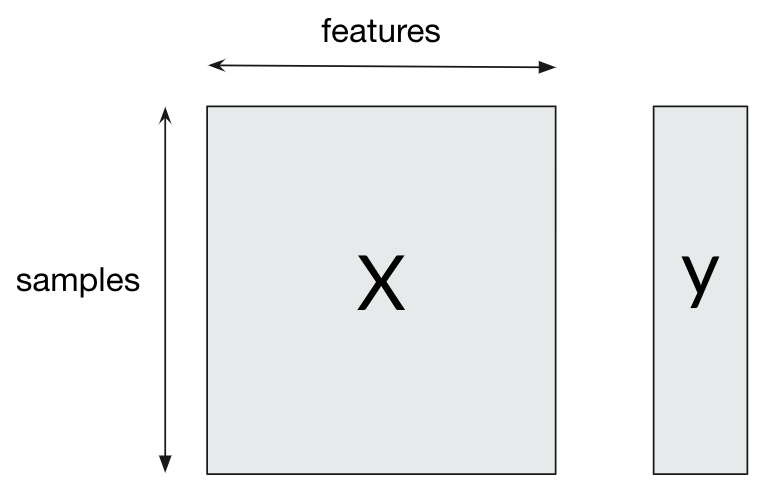
\includegraphics[width=0.7\textwidth]{img/supervised-learning.png}
\end{center}

In \textbf{unsupervised learning}, only the input features are present (i.e. no \emph{y}) and the algorithm learns to recognize patterns, clusters, or other structure in the inputs. Although they're almost never referred to using this terminology, clinical studies that examine the effect between one or more exposures and an outcome are examples of supervised learning. Studies that attempt to uncover groups, or clusters, of similar patients or samples are examples of unsupervised learning.

There are also two other types of machine learning. In \textbf{semi-supervised learning}, a small amount of labeled data is used to create a much larger, weakly-labeled set of training data that is then fed to a supervised learning algorithm. In \textbf{reinforcement learning}, an algorithm is trained with a reward system which provides feedback on the quality of the action the system performs in a given situation instead of (as in supervised learning) simply providing the ``right answer''. 

%%%%%%%%%%%%%%%%%%%%%%%%%%%%%%%%%%%%%%%%%%%%%%%%%%%%%%%%%%%%%%%%%%%%%%%%%%%%%%%%




 


\chapter{Classification \label{chapter:classification}}

Classification is a form of \textbf{supervised learning} in which our goal is to learn a mapping between some features, $x$, and an output, $y$. The general setup for supervised learning looks like this:
\begin{center}
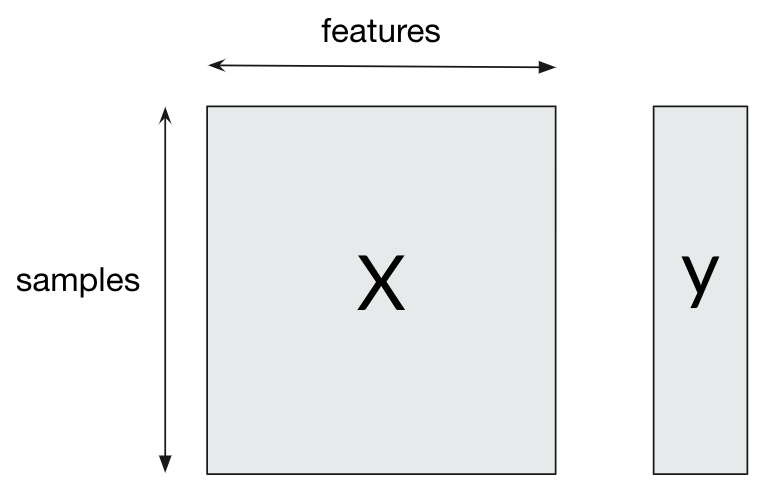
\includegraphics[width=0.7\textwidth]{img/supervised-learning.png}
\end{center}

In classification, the output, $y$, is a category. In \textbf{binary classification} (by far the most common), there are only two categories: yes or no, usually represented as ``0'' (no) or ``1'' (yes). In \textbf{multi-class classification}, there are more than two categories.

To learn an appropriate mapping, we feed \textbf{training data} to a \textbf{learning algorithm}. Different algorithms learn different types of mappings.

\section{Definitions}

\begin{itemize}
\item \textbf{Training data:} The data used, along with an appropriate learning algorithm, to create the mapping between input and output. It is composed of \textbf{samples}, each consisting of one or more input features and a single output.
\item \textbf{Test data:} An independent dataset, not used in model training, on which the performance of a trained supervised learning model is evaluated. 
\item \textbf{Feature:} Also known as a \textbf{predictor}, or \textbf{covariate}, one of the inputs to a supervised learning algorithm.
\item \textbf{Output:} Also known as the \textbf{outcome}, or \textbf{label}, the thing you are trying to predict.
\item \textbf{Feature space:} Envisioning each feature as having its own axis that is orthogonal to all of the other features' axes, the multidimensional space spanned by those axes (or rather: unit vectors in the directions of those axes)
\item \textbf{Extrapolation:} Making predictions outside the region of the feature space occupied by the training data. This will often lead to errors. 
\end{itemize}

%%%%%%%%%%%%%%%%%%%%%%%%%%%%%%%%%%%%%%%%%%%%%%%%%%%%%%%%%%%%%%%%%%%%%%%%%%%%%%%%%%%%%%

\section{Visualizing the Classification Problem \label{section:visualizingclass}}

Imagine we want to predict whether a patient will be readmitted to the emergency room (ER) within $30$~days of discharge from the hospital. We gather data on two predictors: a disease severity score ($x_1$), which characterizes the severity of the illness for which the patient was treated during his/her admission, and a social determinants score ($x_2$), which characterizes a patient's socioeconomic status. We gather data on $200$~distinct patients.

In the figure below, the color refers to whether a patient was admitted to the emergency room (ER) within 30 days of discharge (blue = ``no'', red = ``yes''). The location of each point is governed by the patient's disease severity score ($x_1$, horizontal axis) and social determinants score ($x_2$, vertical axis).

\begin{center}
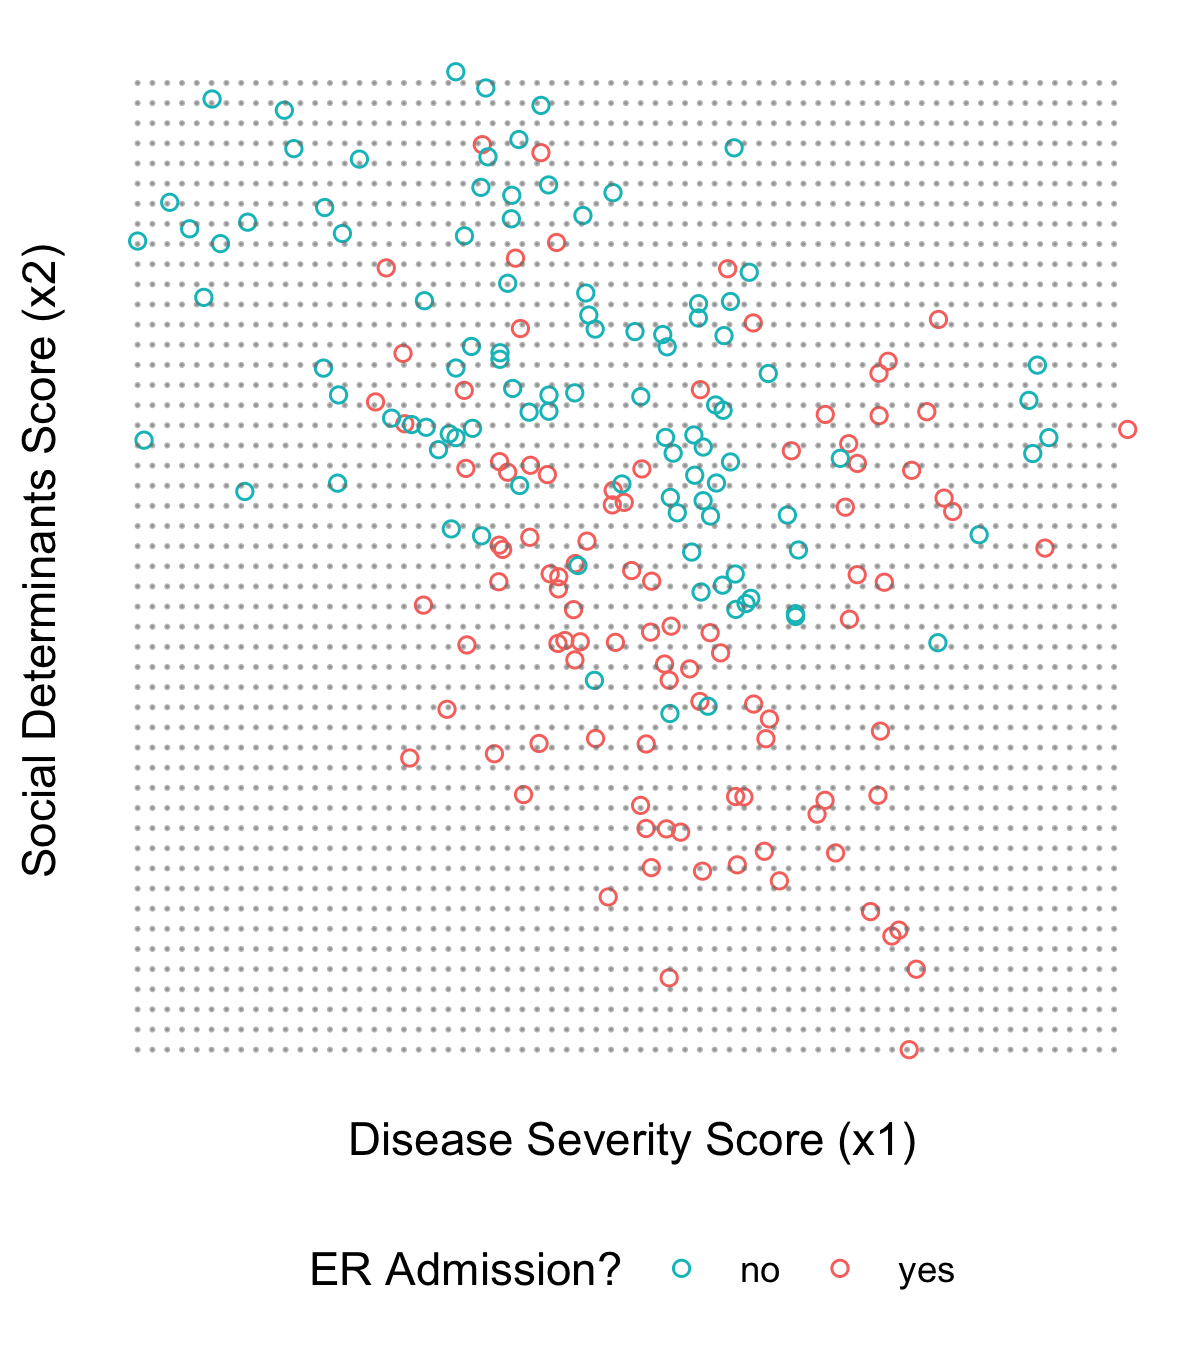
\includegraphics[width=0.7\textwidth]{img/esl-just-data.png}
\end{center}

Our goal in classification is to draw a \textbf{decision boundary}\index{decision boundary} through this space, on one side of which we will predict the patient to be readmitted, and on the other side of which we will predict the patient \emph{not} to be readmitted. The question in classification is: How do we draw a good boundary? How do we draw a boundary that will lead to accurate predictions on patients our model has never seen before?

%%%%%%%%%%%%%%%%%%%%%%%%%%%%%%%%%%%%%%%%%%%%%%%%%%%%%%%%%%%%%%%%%%%%%%%%%%%%%%%%%%%%%%

\section{Three Classification Algorithms}

\subsection{Logistic Regression}

The simplest decision boundary is, arguably, a line. The logistic regression\index{logistic regression} algorithm simply draws a line\footnote{In a higher-dimensional feature space, the decision boundary for logistic regression is a \textbf{hyperplane}.} through the feature space that divides the positive and negative training examples. 

\begin{center}
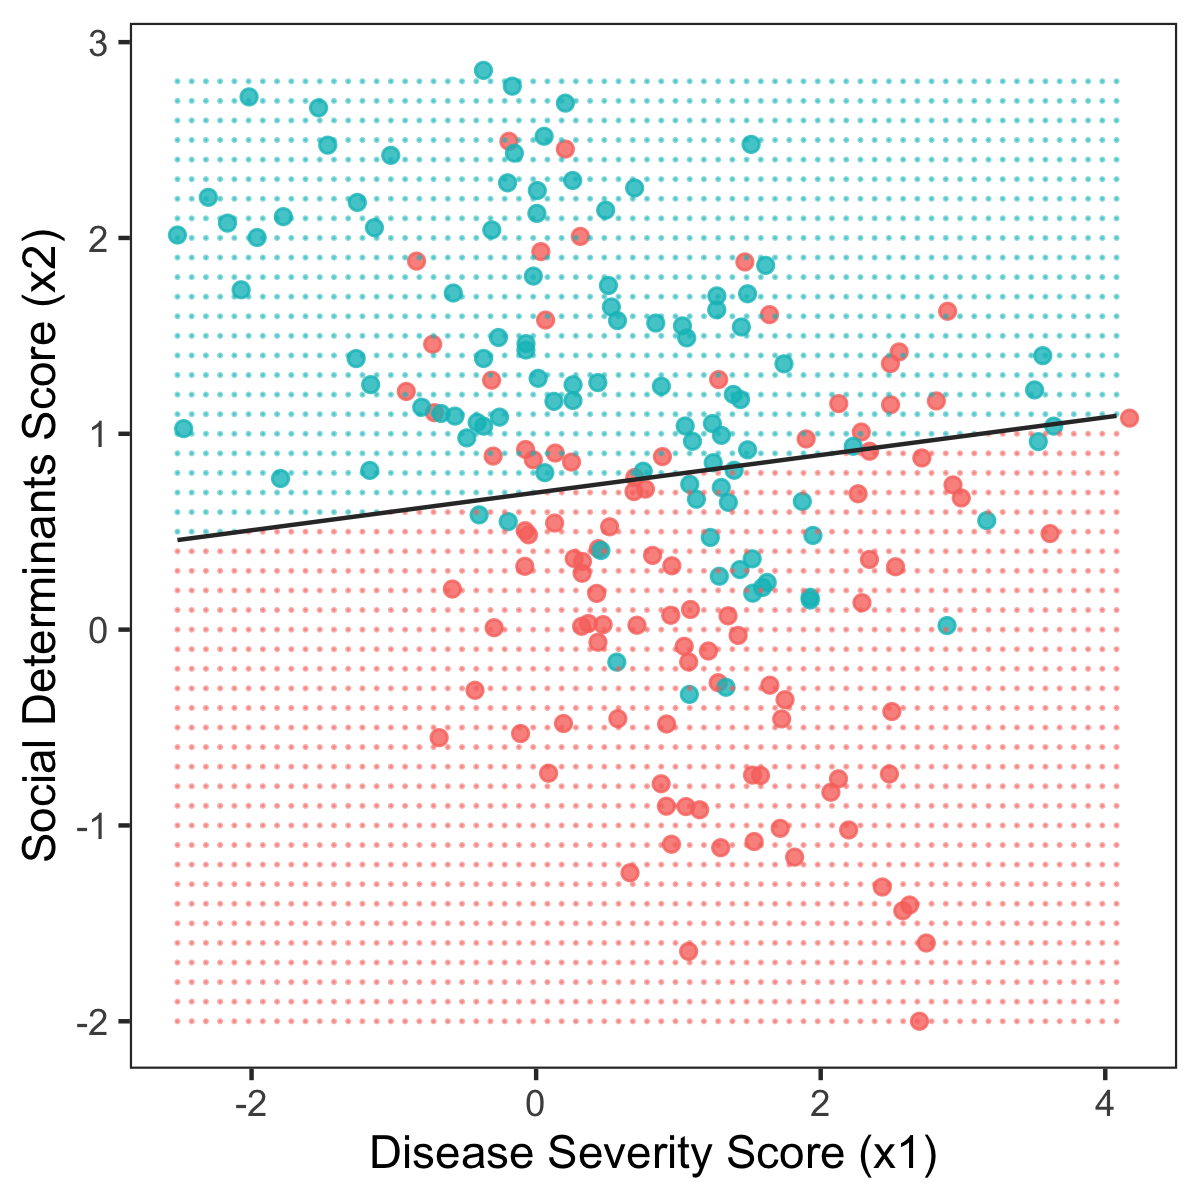
\includegraphics[width=0.7\textwidth]{img/esl-logistic.png}
\end{center}

\subsection{K Nearest Neighbors (KNN)}

Another approach is to make no assumptions about the shape of the decision boundary. To make a prediction about a new patient, we simply allow the $K$ nearest neighbors to vote. The parameter $K$ must be set independently and is called a \textbf{hyperparameter}. 

\noindent Here is the decision boundary for KNN with $K=15$:
\begin{center}
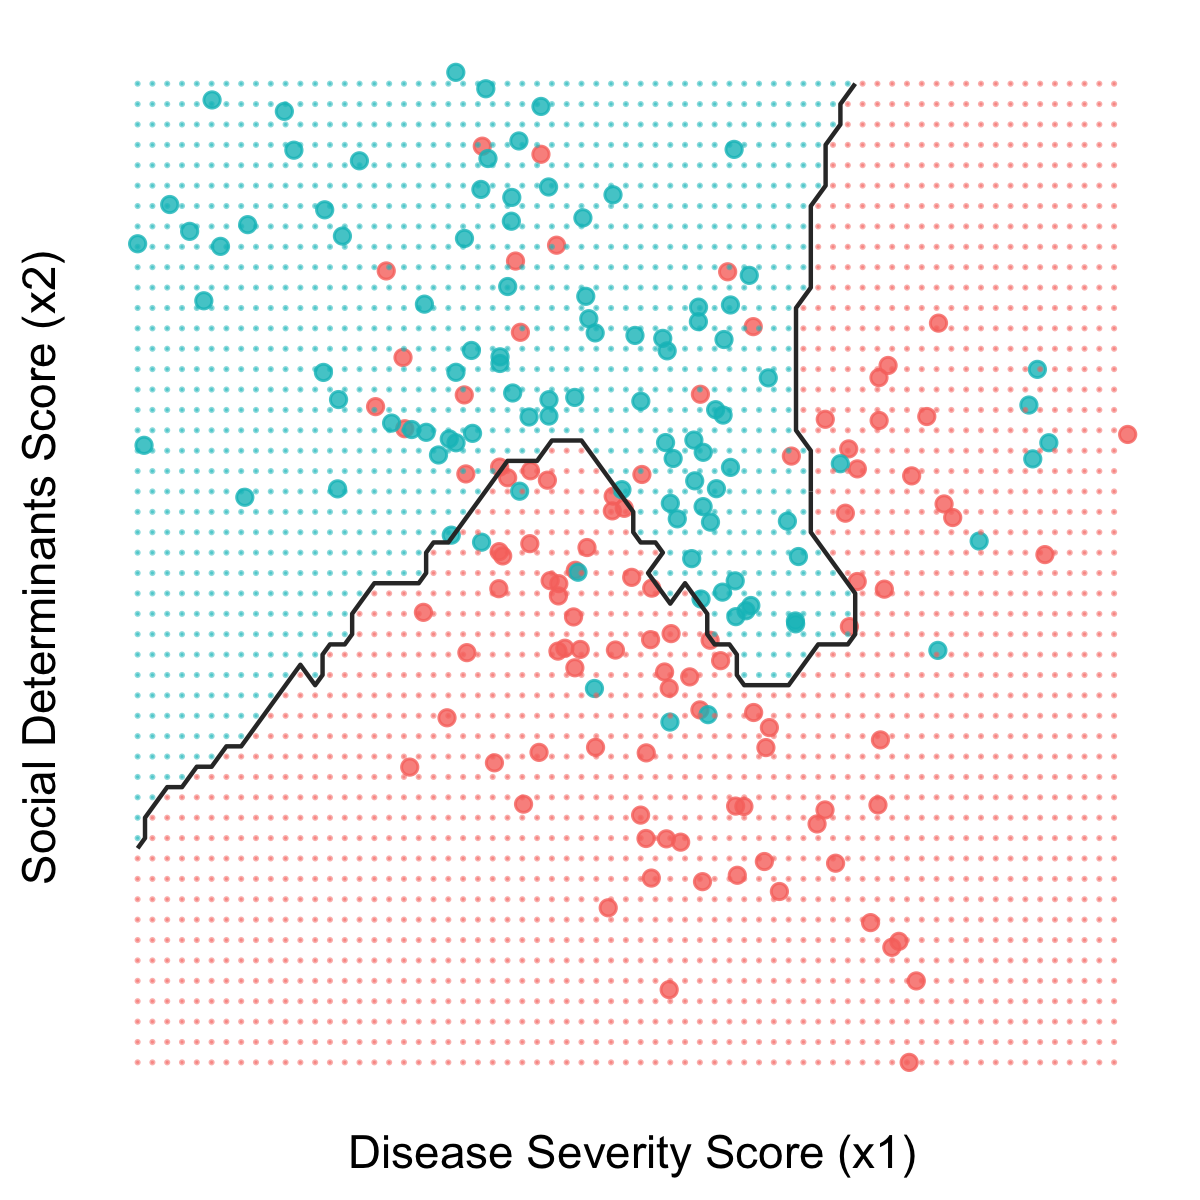
\includegraphics[width=0.7\textwidth]{img/esl-knn-15.png}
\end{center}

\subsection{Decision Tree}

Finally, we may choose to use our training data to build a decision tree\index{decision tree}, which will allow us to make predictions on new patients using a series of simple yes/no questions. There are different decision tree learning algorithms, but here is the tree produced by a famous one called CART:
\begin{center}
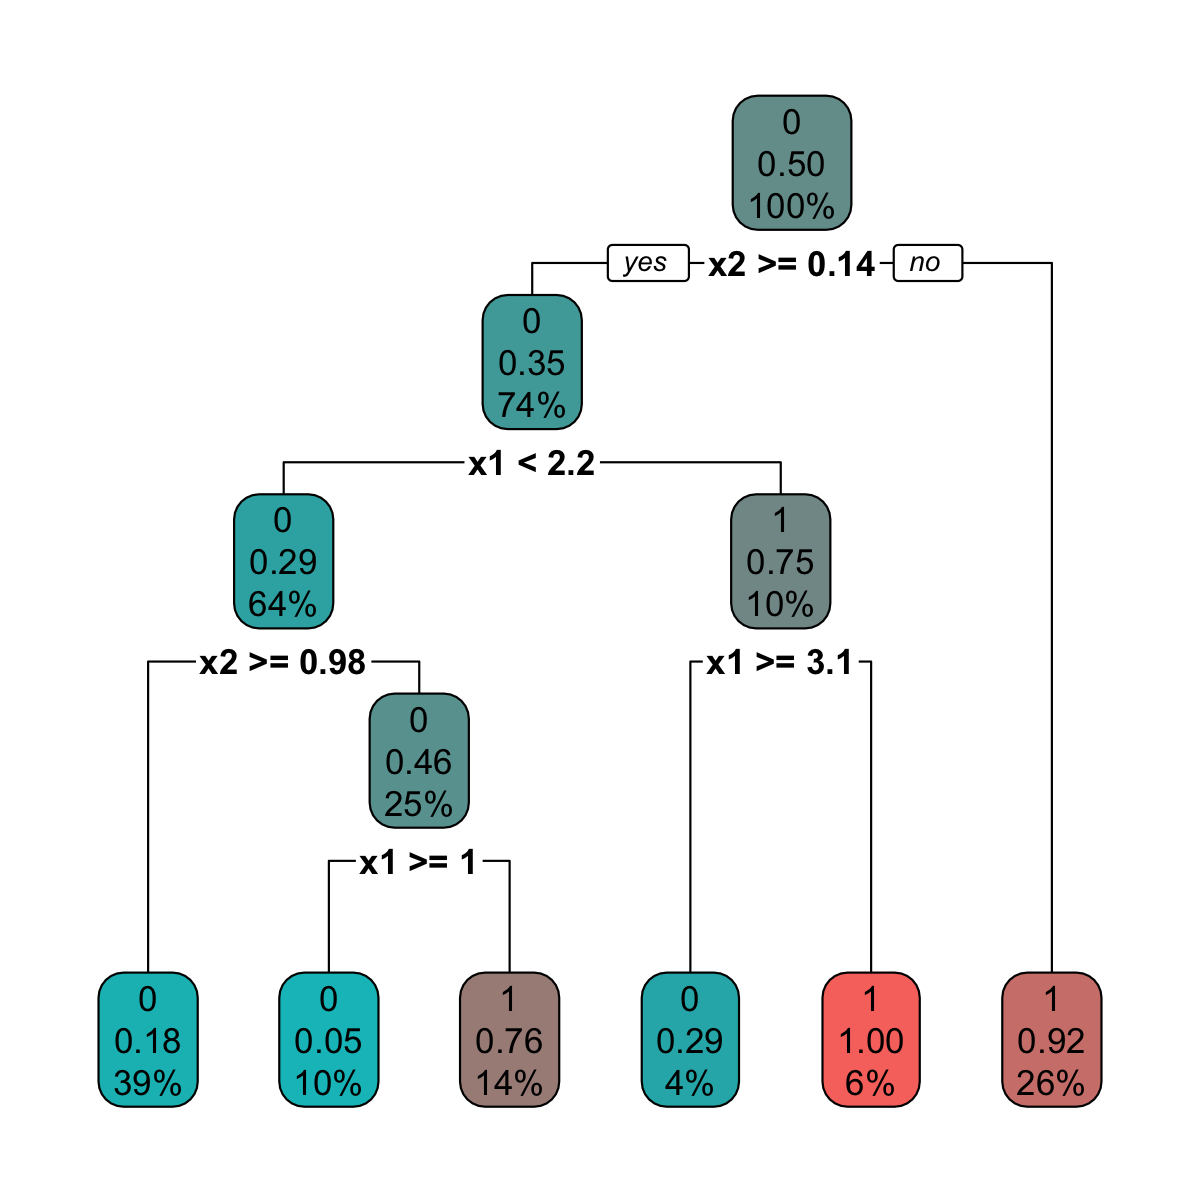
\includegraphics[width=0.6\textwidth]{img/esl-decision-tree-just-tree.png}
\end{center}
And here is the decision boundary produced by this tree:
\begin{center}
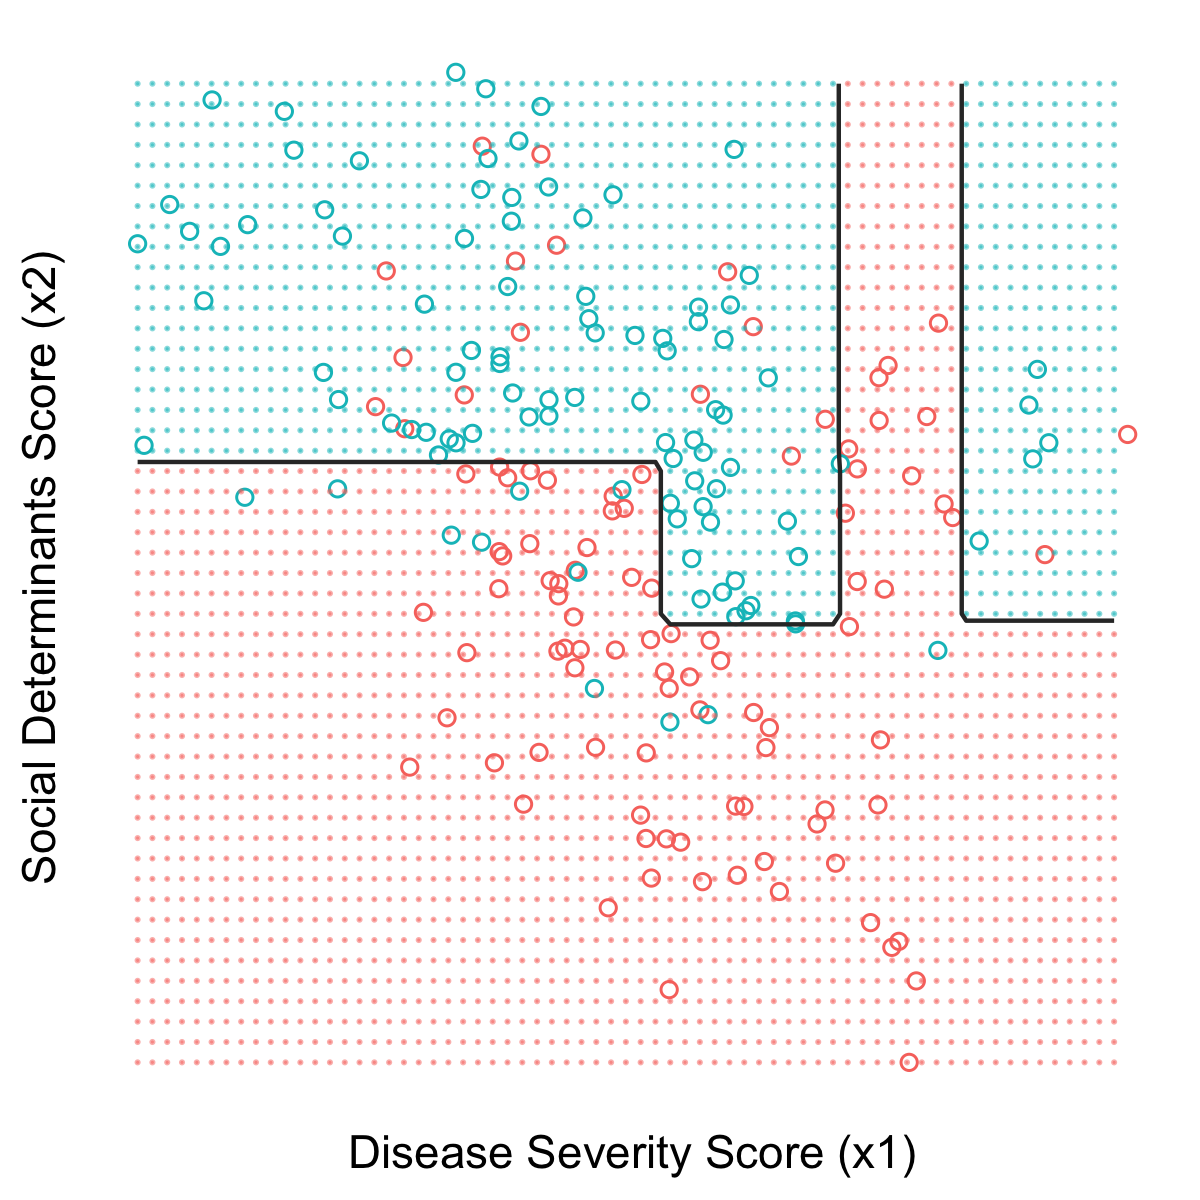
\includegraphics[width=0.7\textwidth]{img/esl-decision-tree.png}
\end{center}

%%%%%%%%%%%%%%%%%%%%%%%%%%%%%%%%%%%%%%%%%%%%%%%%%%%%%%%%%%%%%%%%%%%%%%%%%%%%%%%%%%%%%%

\section{Classification with Probabilities}

We can think of classification as simply drawing a decision boundary, but beneath each algorithm is a quantitative assessment of each point in the feature space. Each algorithm is, in its own way, able to provide a degree of certainty, or probability, that a point belongs to the positive or negative class. For example, here is the feature space of the example we just saw, colored by the probability (according to logistic regression) that a sample at each point should be classified as positive or negative: 

\begin{center}
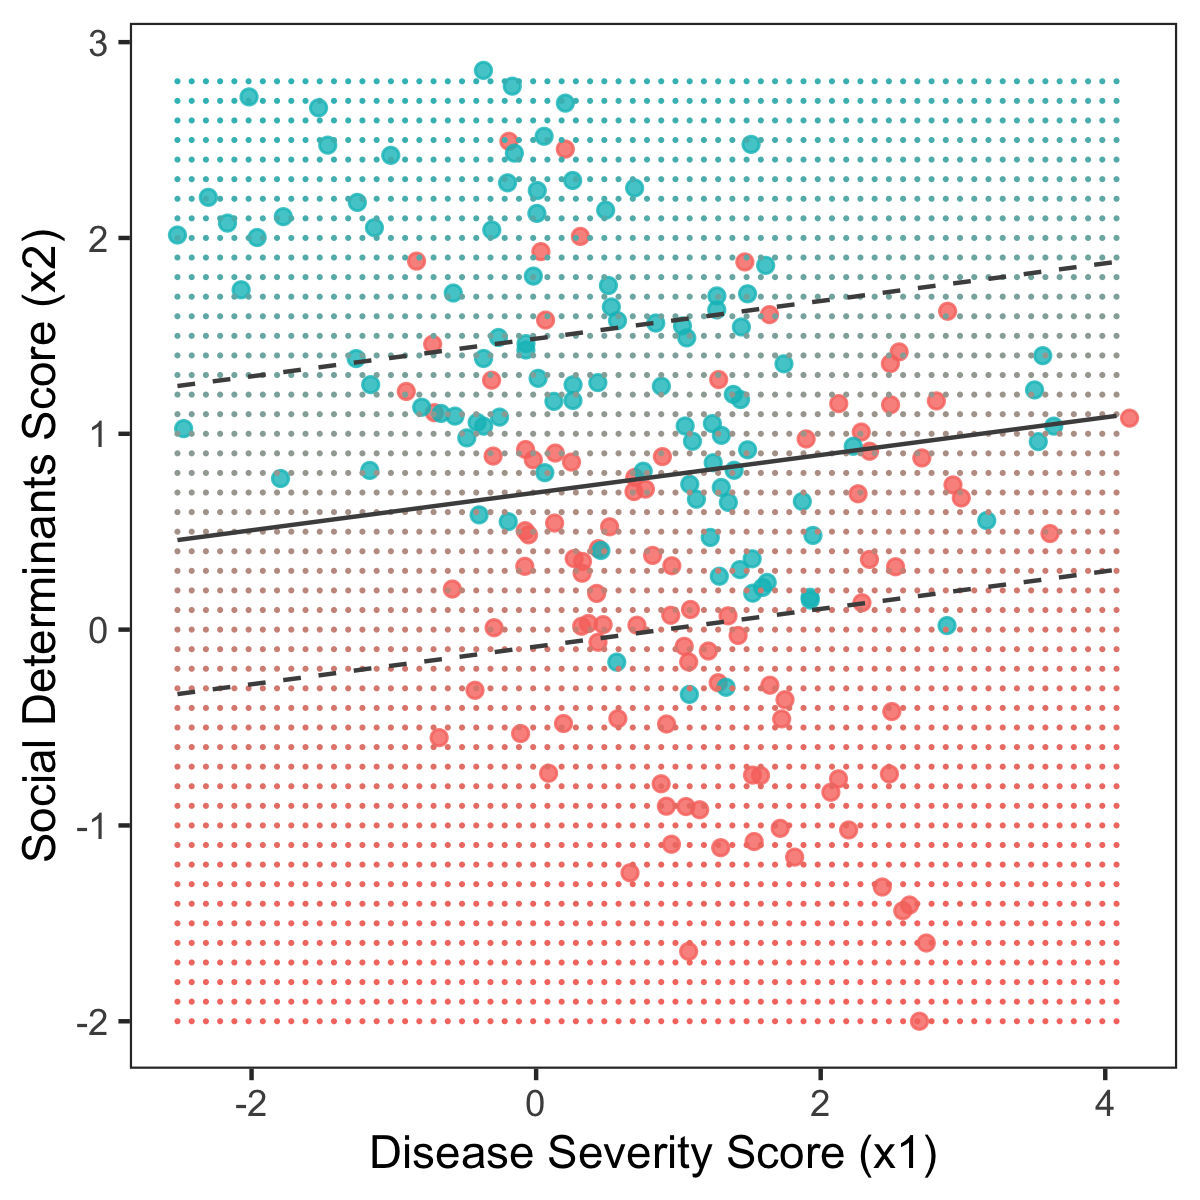
\includegraphics[width=0.7\textwidth]{img/esl-logistic-prob.png}
\end{center}

\noindent Here is a plot of probabilities for KNN ($K=15$): 
\begin{center}
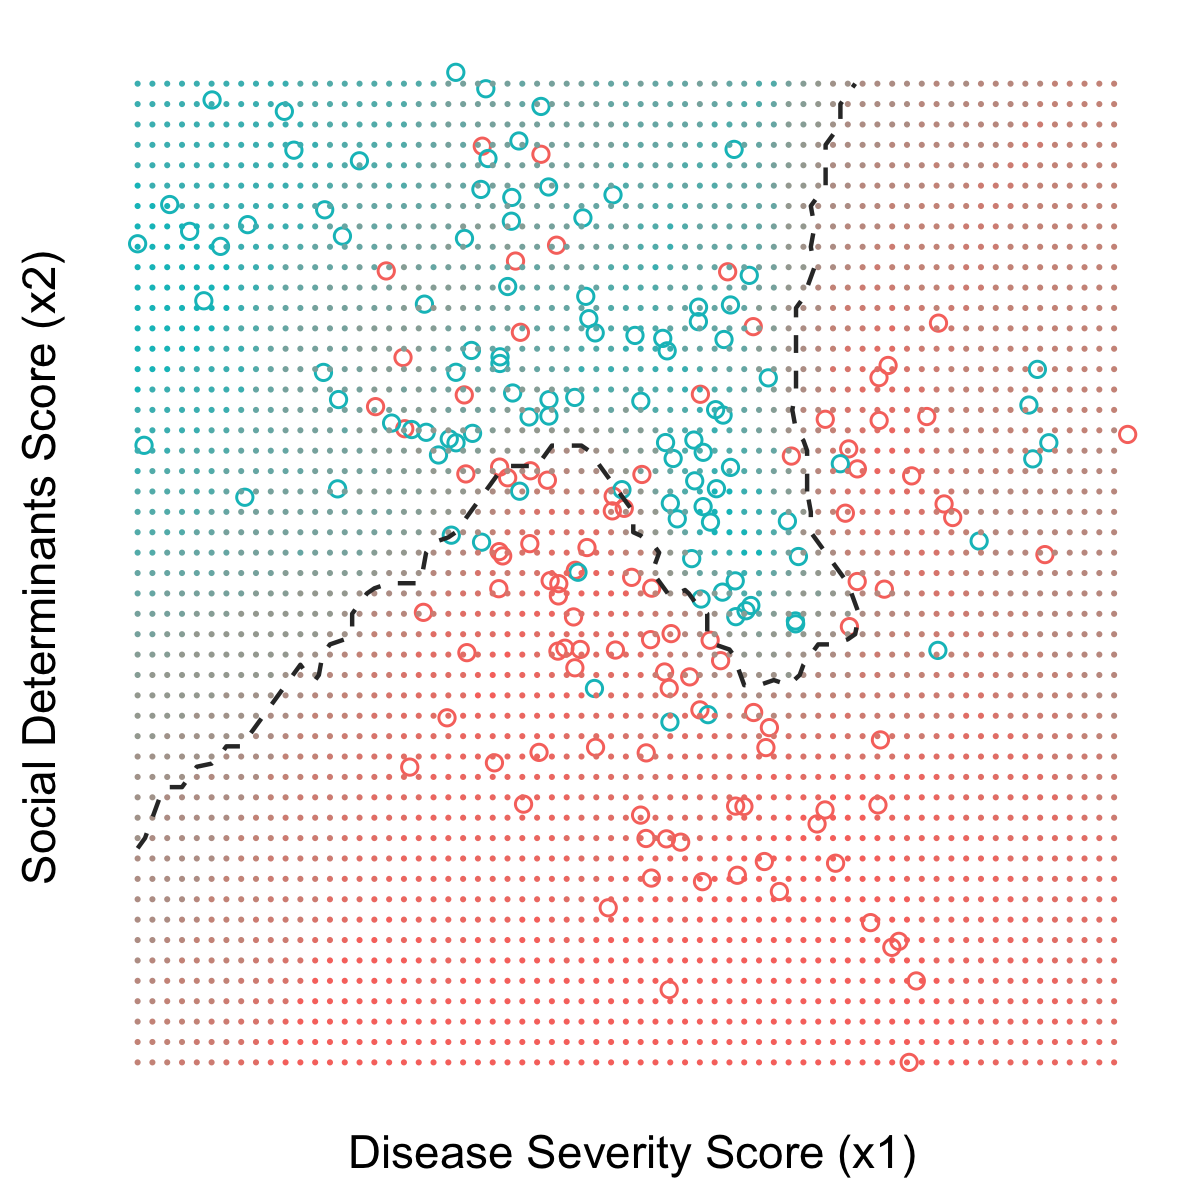
\includegraphics[width=0.68\textwidth]{img/esl-knn-15-prob.png}
\end{center}

\noindent And here is a plot of probabilities for the decision tree:
\begin{center}
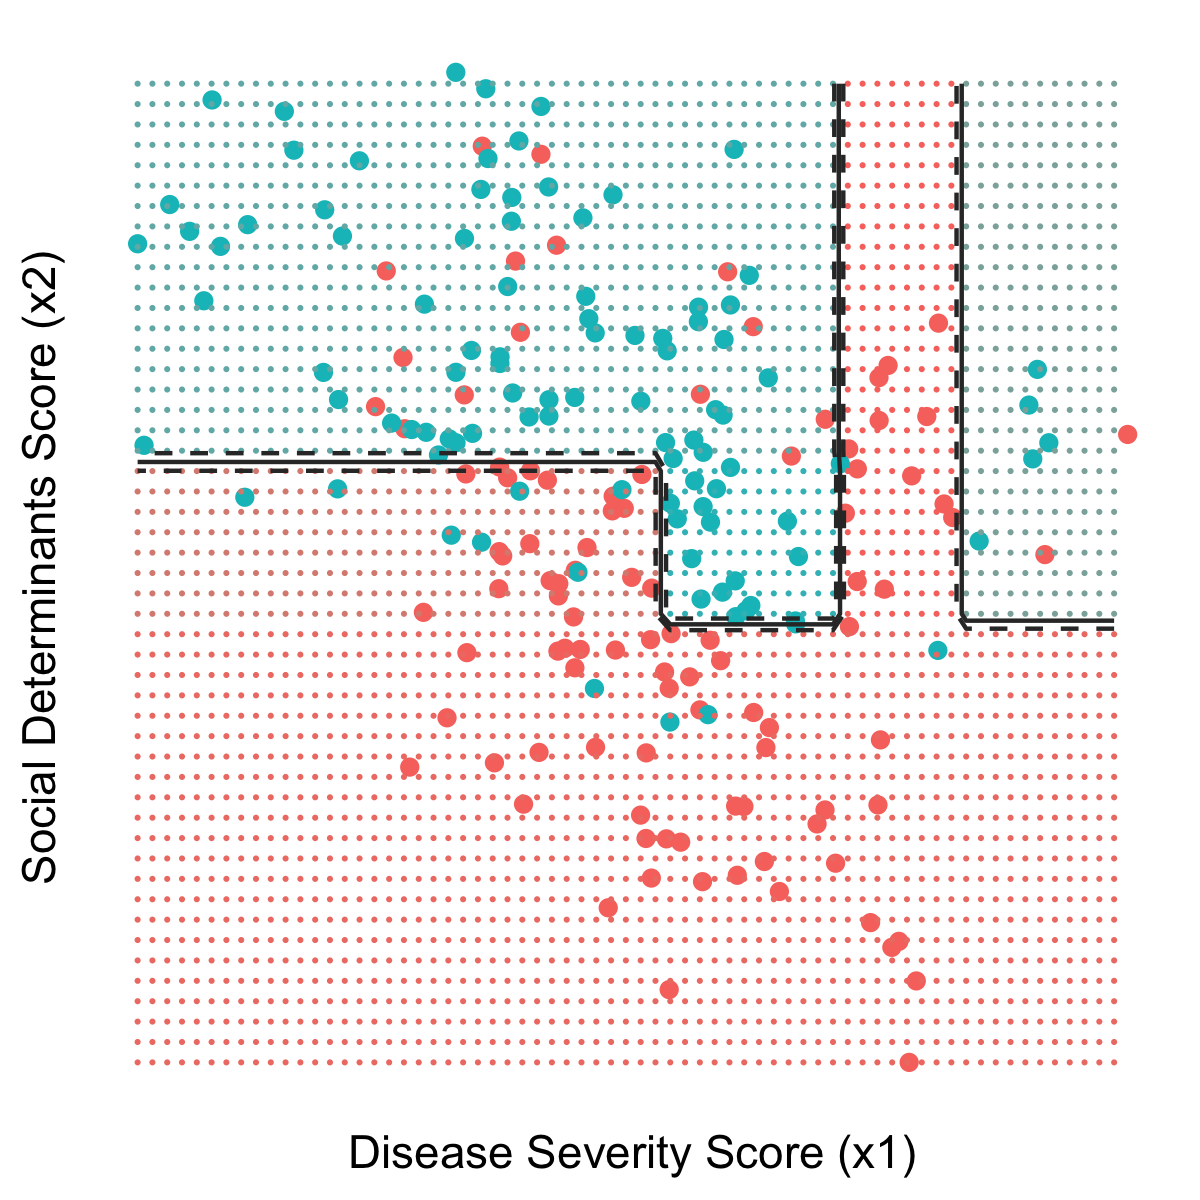
\includegraphics[width=0.68\textwidth]{img/esl-decision-tree-prob.png}
\end{center}

%%%%%%%%%%%%%%%%%%%%%%%%%%%%%%%%%%%%%%%%%%%%%%%%%%%%%%%%%%%%%%%%%%%%%%%%%%%%%%%%%%%%%%

\section{Discussion Questions}

Logistic regression, KNN, and decision trees are three distinct types of classification algorithms. Fed the same training data, they produce three very different-looking decision boundaries.

\begin{enumerate}
\item What are the advantages and disadvantages of the decision boundaries produced by:
  \begin{enumerate}
  \item Logistic regression?
  \item KNN ($K=15$)?
  \item Decision tree?
  \end{enumerate}
\item What are the advantages and disadvantages of KNN with low $K$ (e.g. $K=3$) vs. high $K$ (e.g. $K=50$)? The decision boundaries for the previous example with (left to right) $K=3, 15,$ and $50$ are shown below.
\begin{center}
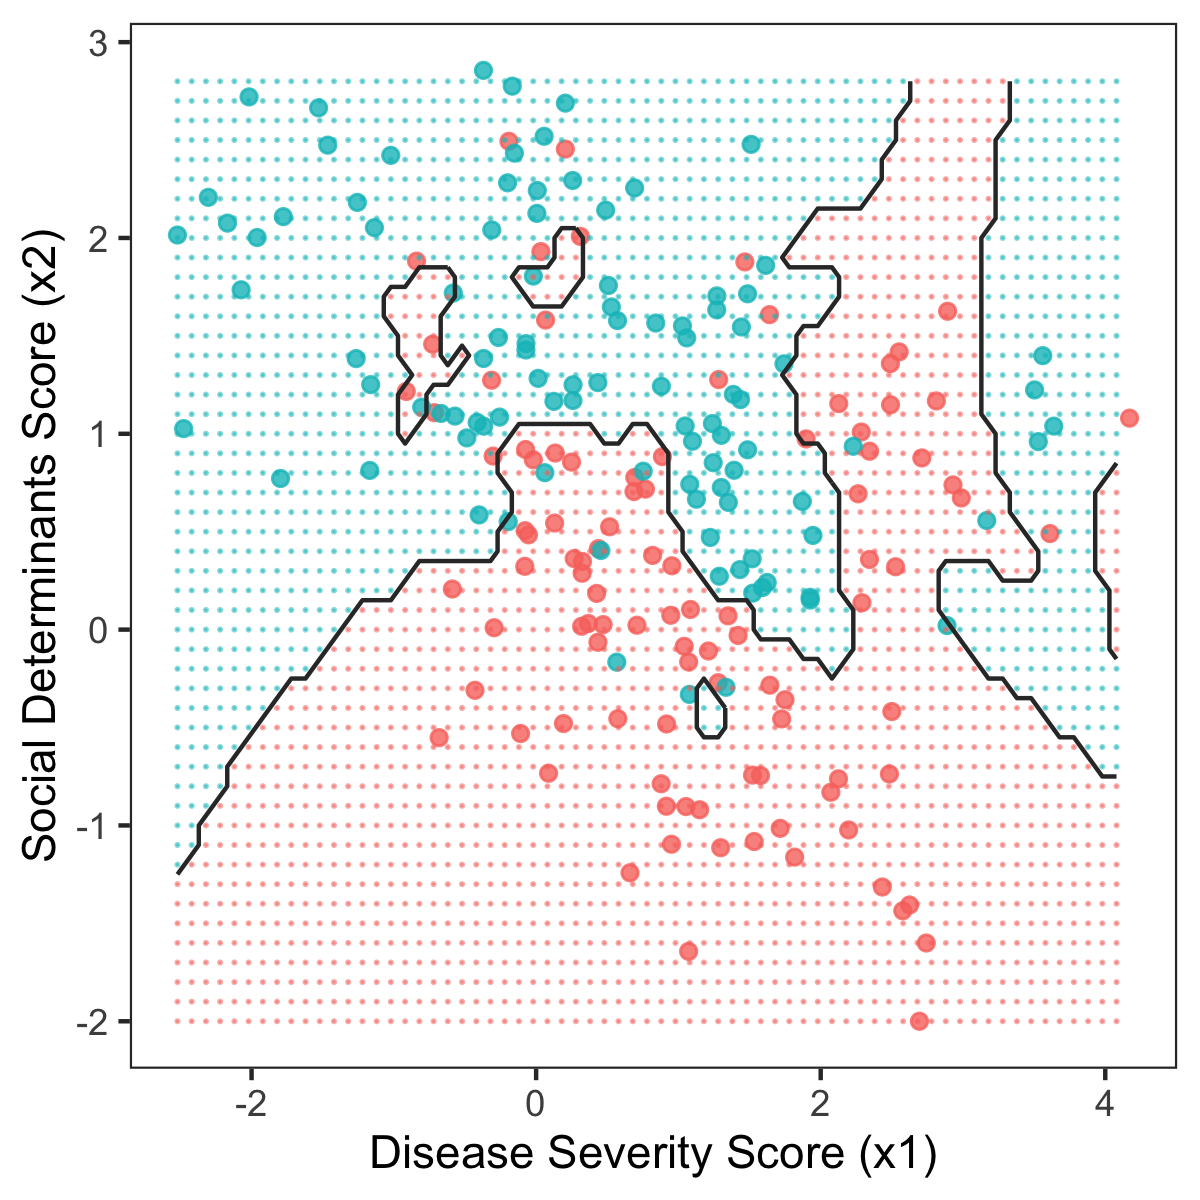
\includegraphics[width=0.3\textwidth]{img/esl-knn-3.png}
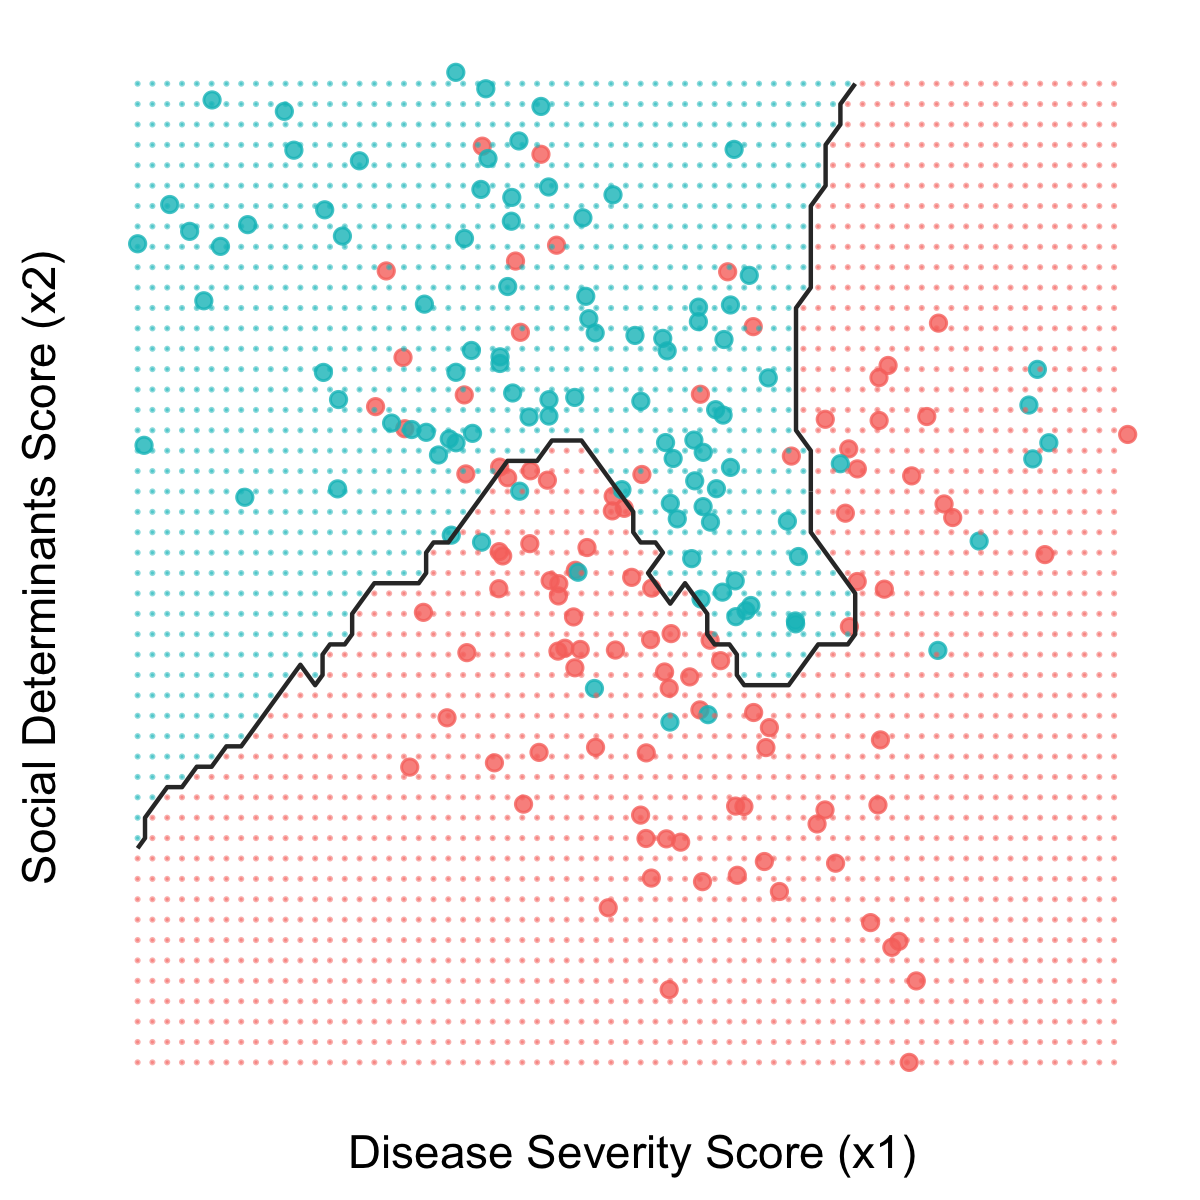
\includegraphics[width=0.3\textwidth]{img/esl-knn-15.png}
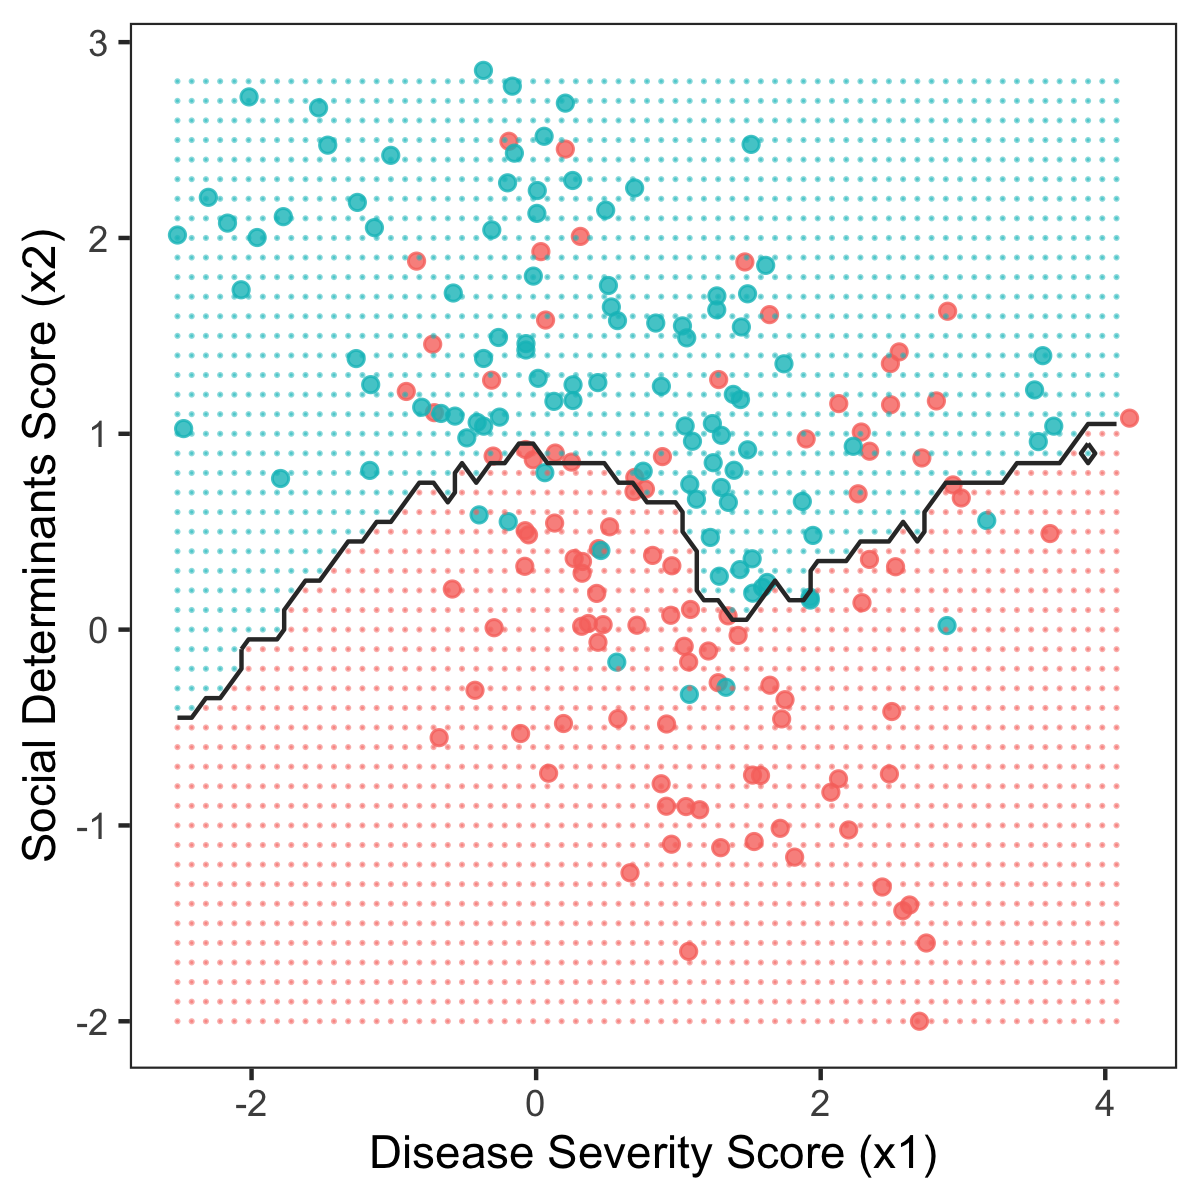
\includegraphics[width=0.3\textwidth]{img/esl-knn-50.png}
\end{center}
\item What makes a good classification algorithm?
\item The logistic regression, KNN, and decision tree algorithms can all be applied to address multi-outcome (i.e. more than two categories) classification problems with only minor modifications. Describe how each could be modified to work in these situations. (Think through this yourself before you Google.)
\end{enumerate}




\chapter{Regression \label{chapter:regression}}

Classification is a form of supervised learning in which the outcome is a category. \textbf{Regression}\index{regression} is another form of supervised learning in which the outcome is a numeric value. For example, it may be a lab value, physical characteristic (height, weight, etc.), or numeric measurement (e.g. oxygen saturation).

%%%%%%%%%%%%%%%%%%%%%%%%%%%%%%%%%%%%%%%%%%%%%%%%%%%%%%%%%%%%%%%%%%%%%%%%%%%%%%%%%%%%%%

\section{Visualizing the Regression Problem \label{section:visualizingreg}}

Let's consider the same setup from Section~\ref{section:visualizingclass} but this time with a quantitative outcome: a ``recurrence biomarker'' that indicates the likelihood of recurrence of disease.

Again, we have data on two predictors: a disease severity score ($x_1$), which characterizes the severity of the illness for which the patient was originally treated, and a social determinants score ($x_2$), which characterizes a patient's socioeconomic status. We have data on the same $200$ patients that we examined in Section~\ref{section:visualizingclass}. 

\begin{center}
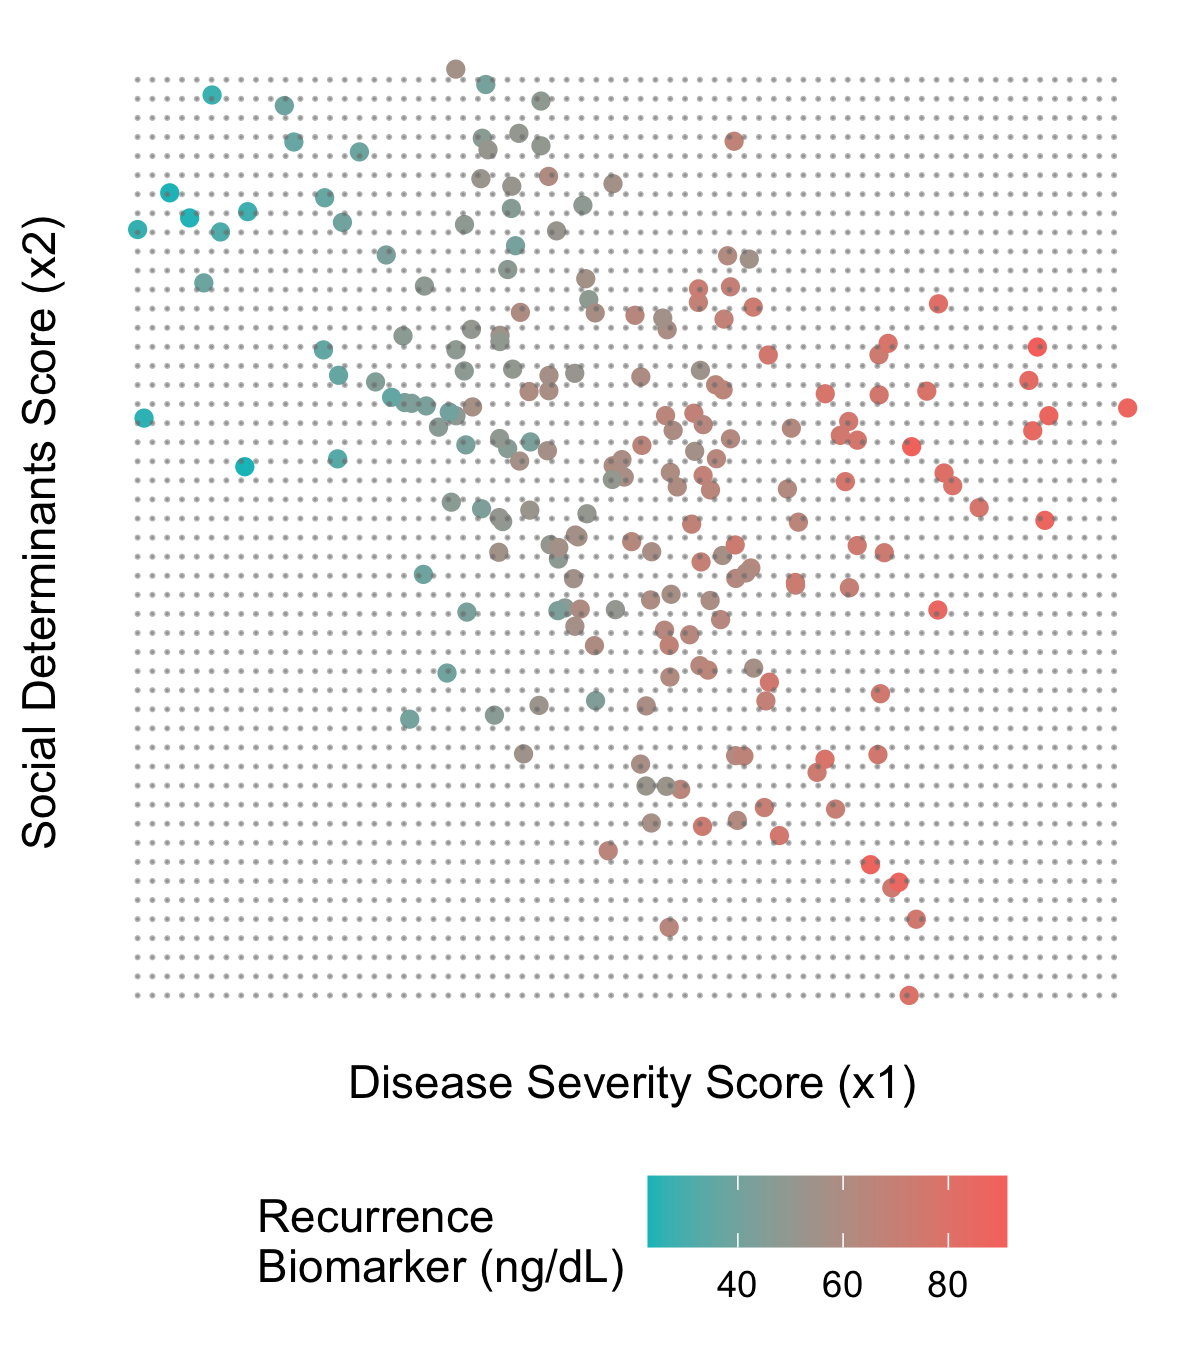
\includegraphics[width=0.65\textwidth]{img/esl-reg-just-data.png}
\end{center}

This is a plot of the data in a single plane. You can also view the data in 3D; here the color is redundant, since the height above the $x_1 \times x_2$ plane is represented separately.

\begin{center}
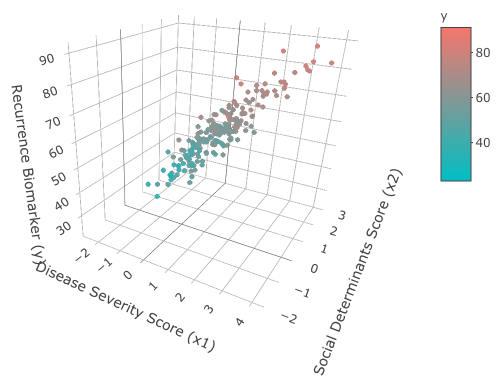
\includegraphics[width=0.7\textwidth]{img/esl-reg-3d-view-2.png}
\end{center}

%%%%%%%%%%%%%%%%%%%%%%%%%%%%%%%%%%%%%%%%%%%%%%%%%%%%%%%%%%%%%%%%%%%%%%%%%%%%%%%%%%%%%%

\section{Discussion Questions}

Think about the three algorithms we discussed in Chapter~\ref{chapter:classification}. Now think about our new task, which is to predict the \emph{numeric value} of the recurrence biomarker as a function of the two predictors, $x_1$ and $x_2$. 

\begin{enumerate}
\item Just looking at the two predictors, which one appears to more highly influence the value of the recurrence biomarker? Why?
\item How might you adapt KNN to deal with this problem?
\item How might you adapt a decision tree to deal with this problem?
\item How might you adapt logistic regression to deal with this problem? You'll have to ``break the algorithm'' a bit more this time.  
\item These plots are the regression equivalents of the plots we made in Chapter~\ref{chapter:classification}. They need to be 3D so you can see the geometry of the predictions more clearly. One contains predictions from KNN with $K=15$, one contains predictions from a decision tree, and one contains predictions from an algorithm called \textbf{linear regression}, which is a relative of logistic regression. Which algorithm goes with which plot?
\begin{center}
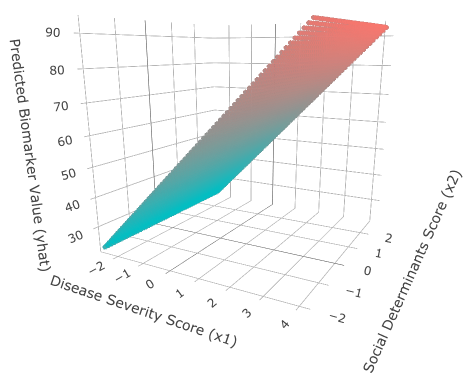
\includegraphics[width=0.7\textwidth]{img/esl-reg-3d-linear-small.png}
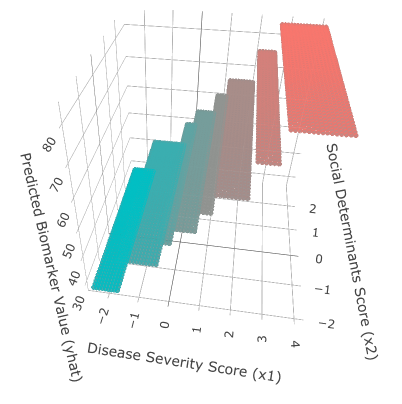
\includegraphics[width=0.6\textwidth]{img/esl-reg-3d-decision-tree-small.png}
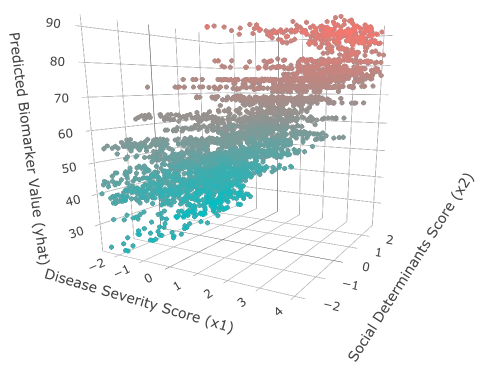
\includegraphics[width=0.7\textwidth]{img/esl-reg-3d-knn-15-small.png}
\end{center}
\item What are the advantages and disadvantages of each regression algorithm?
\item How could classification be viewed as ``just another form of regression''?
\end{enumerate}


\chapter{Probability Distributions \label{chapter:probabilitydistributions}}

Many of the methods we will examine in these workshops depend on basic concepts from probability theory. For example, linear and logistic regression are members of a class of supervised learning algorithms called \textbf{generalized linear models} (see Chapter~\ref{chapter:glms}) which make assumptions about the type of probability distribution followed by the outcome variable. Decision trees use a concept called \textbf{entropy} (see Chapter~\ref{chapter:decisiontrees}), whose mathematical formulation depends on the probability distribution underlying the outcome. Many \textbf{hypothesis tests} (see Chapter~\ref{chapter:hypothesistesting}) likewise rely on probabilistic assumptions about the data. Probability is everywhere.

The following sections review some key probability concepts -- in an extremely hand-wavey and non-rigorous way -- and the properties of some of the most common probability distributions you will encounter in machine learning and statistics. 

\section{Definitions}

A \textbf{probability distribution} is just a mathematical function that provides the relative likelihoods of various possible outcomes of an observation. We call the quantity that is being observed a \textbf{random variable}. Probability distributions can be discrete or continuous. The random variable involved can be a number, a vector of numbers, a category/class, etc. The \textbf{sample space} is the set of all possible outcomes. The integral (or sum) of the probability distribution over the entire sample space is $1.0$. You will often hear probability distributions for continuous random variables referred to as \textbf{probability densities}. 

Probability distributions are grouped into families that are characterized by their overall shapes. These families contain \textbf{parameters} that, when varied, produce different distributions. Specific probability distributions from within a single family can often look quite different. 

We use the notation $E[x|\theta]$ to refer to the \textbf{expected value}, or mean, of a distribution, given its parameter(s), $\theta$. There can be more than one parameter, and it will not always be called $\theta$; this is just an example. We use the notation $\text{var}(x|\theta)$ to refer to the \textbf{variance}, or spread, of a distribution around its mean. 

\section{Normal Distribution \label{sect:normal}} 

Also called the \textbf{Gaussian distribution}, the normal distribution is probably the most well-known continuous probability distribution. It has the following properties:
\begin{equation*} p(x | \mu, \sigma) = \frac{1}{\sqrt{2 \pi \sigma^2}} e^{-\frac{(x-\mu)^2}{2 \sigma^2}} \qquad  E[x| \mu, \sigma] = \mu \qquad \text{var}(x | \mu, \sigma) = \sigma^2 \end{equation*}
where $x \in \mathbb{R}$. We will abbreviate the normal distribution as $\mathcal{N}(\mu, \sigma)$.  The value of $\mu$ changes the position of the center of the normal distribution.
\begin{center}
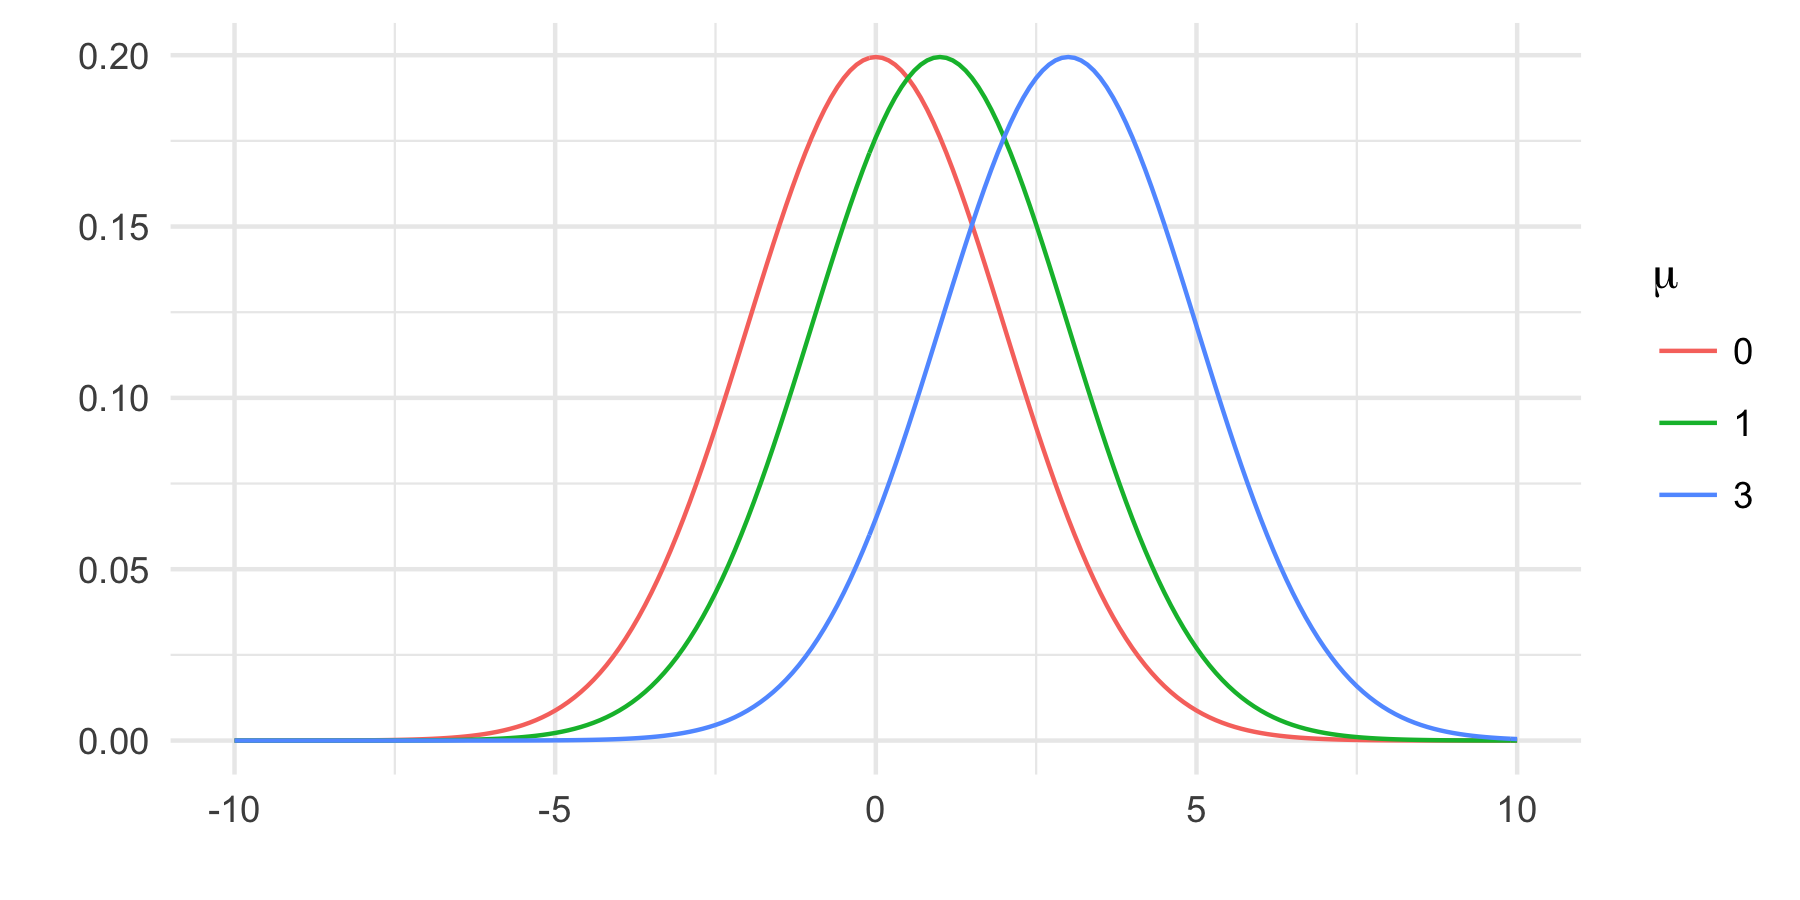
\includegraphics[width=0.9\textwidth]{img/l01-figure1a-normal-mean-change.png}
\end{center}
The value of $\sigma$ changes the width of the normal distribution.
\begin{center}
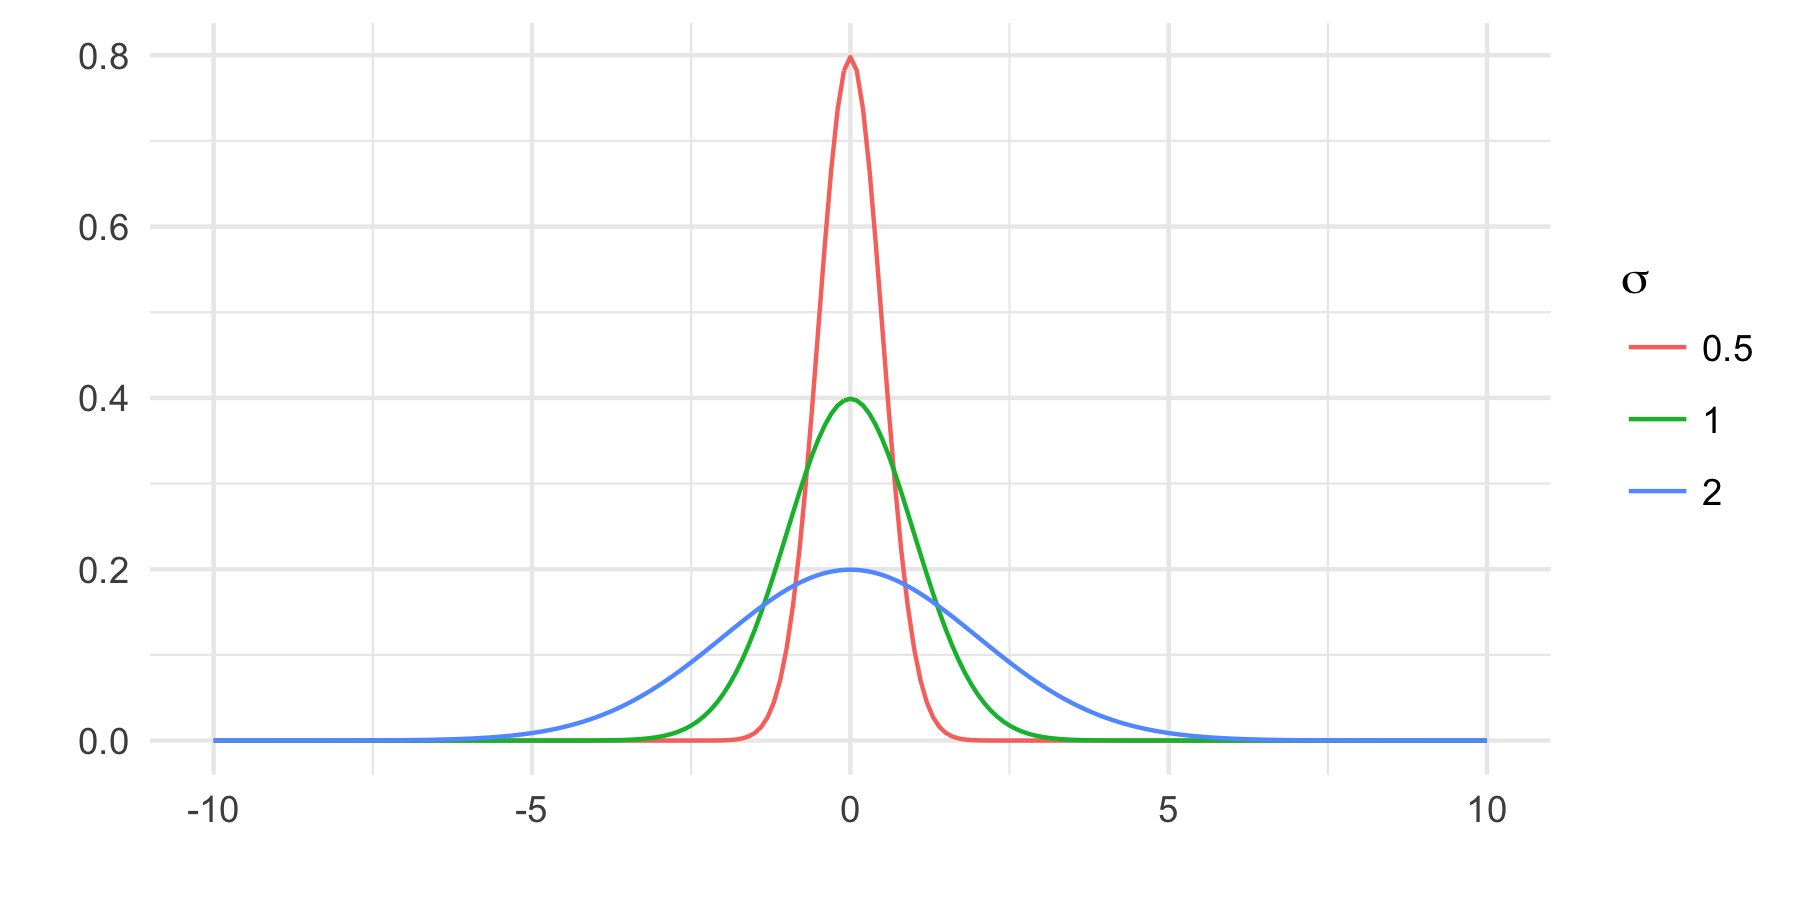
\includegraphics[width=0.9\textwidth]{img/l01-figure1b-normal-sd-change.png}
\end{center}

\begin{question}{question:normalex}
List 5 random variables from medicine or biology that should follow normal distributions.
\end{question}
 

\section{Bernoulli Distribution \label{sect:bernoulli}}

The \textbf{Bernoulli distribution} is a discrete probability distribution with the following properties:
$$ p(x|\mu) = \mu^x (1 - \mu) ^ {1-x} \qquad E[x| \mu] = \mu \qquad \text{var}(x | \mu) = \mu (1 - \mu) $$
where $x \in \{0, 1\}$. It is used to model events where the outcome is yes/no. Think of it as a weighted coin, with $\mu$ the probability that the coin comes up ``heads'' on a single toss. Here are three Bernoulli distributions with (from left to right) $\mu = 1.0, 0.7, 0.2$. The number along the bottom is $x$, which can only be $0$ or $1$. 
\begin{center}
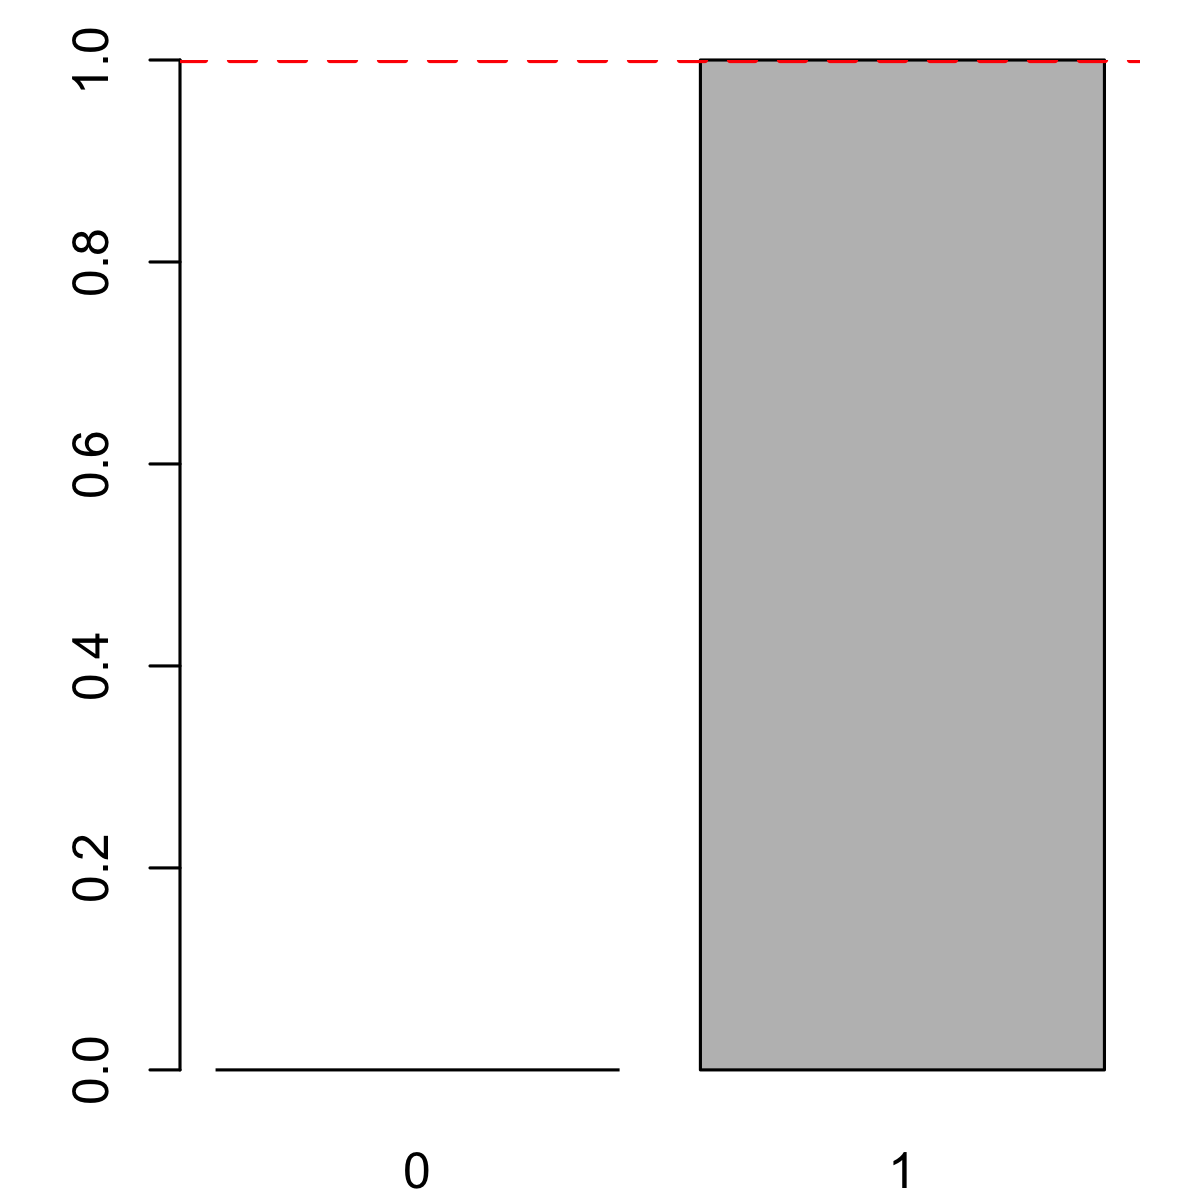
\includegraphics[width=0.3\textwidth]{img/l01-figure2a-bernoulli-1-0.png}
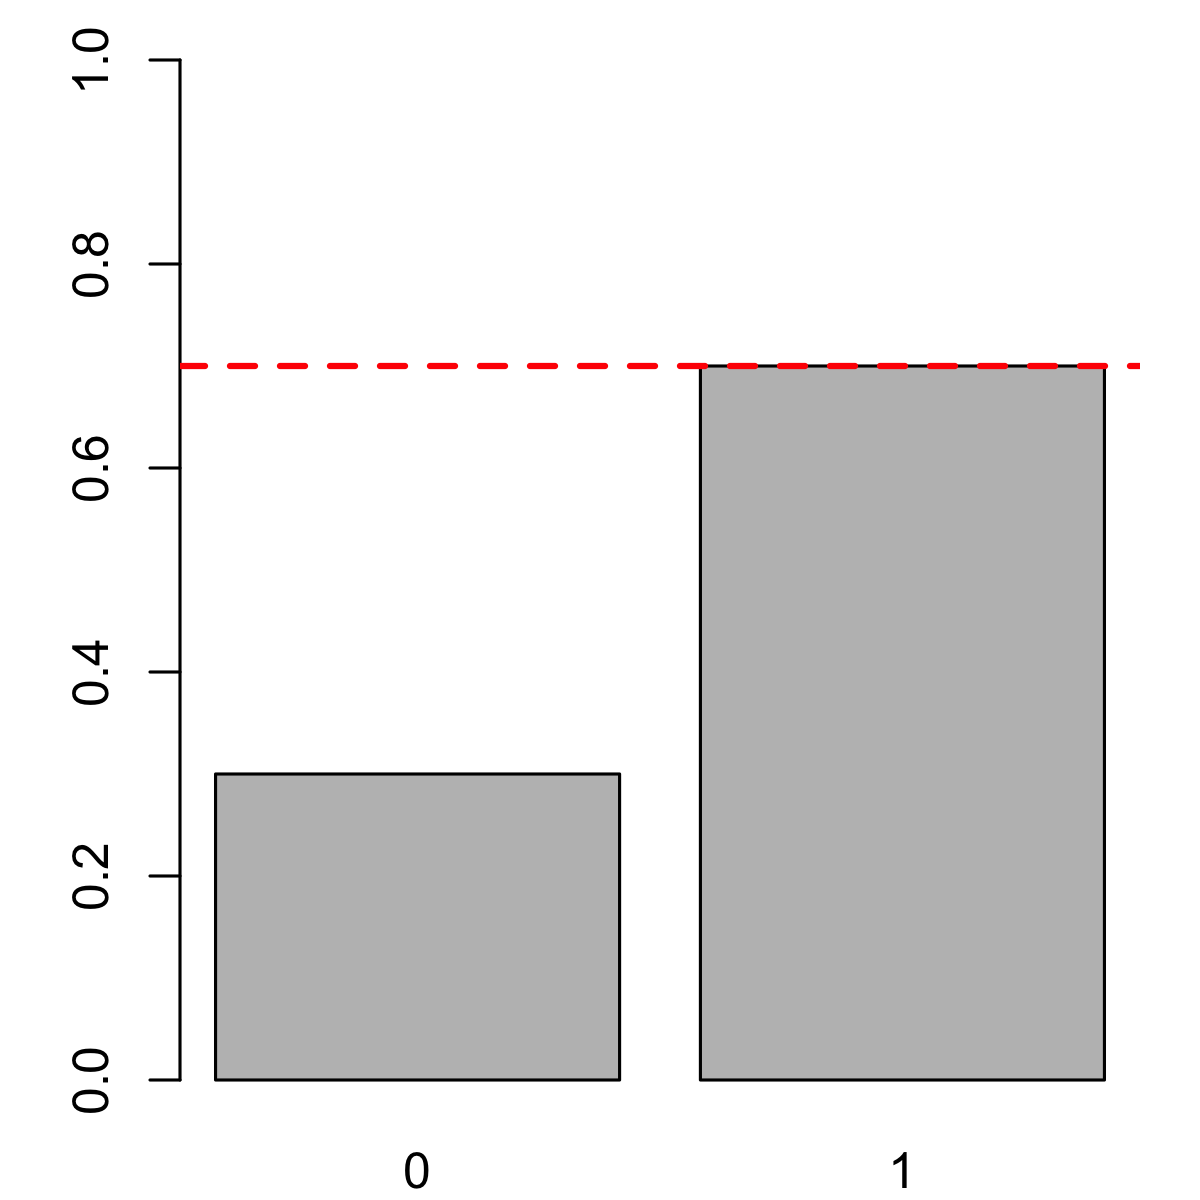
\includegraphics[width=0.3\textwidth]{img/l01-figure2b-bernoulli-0-7.png}
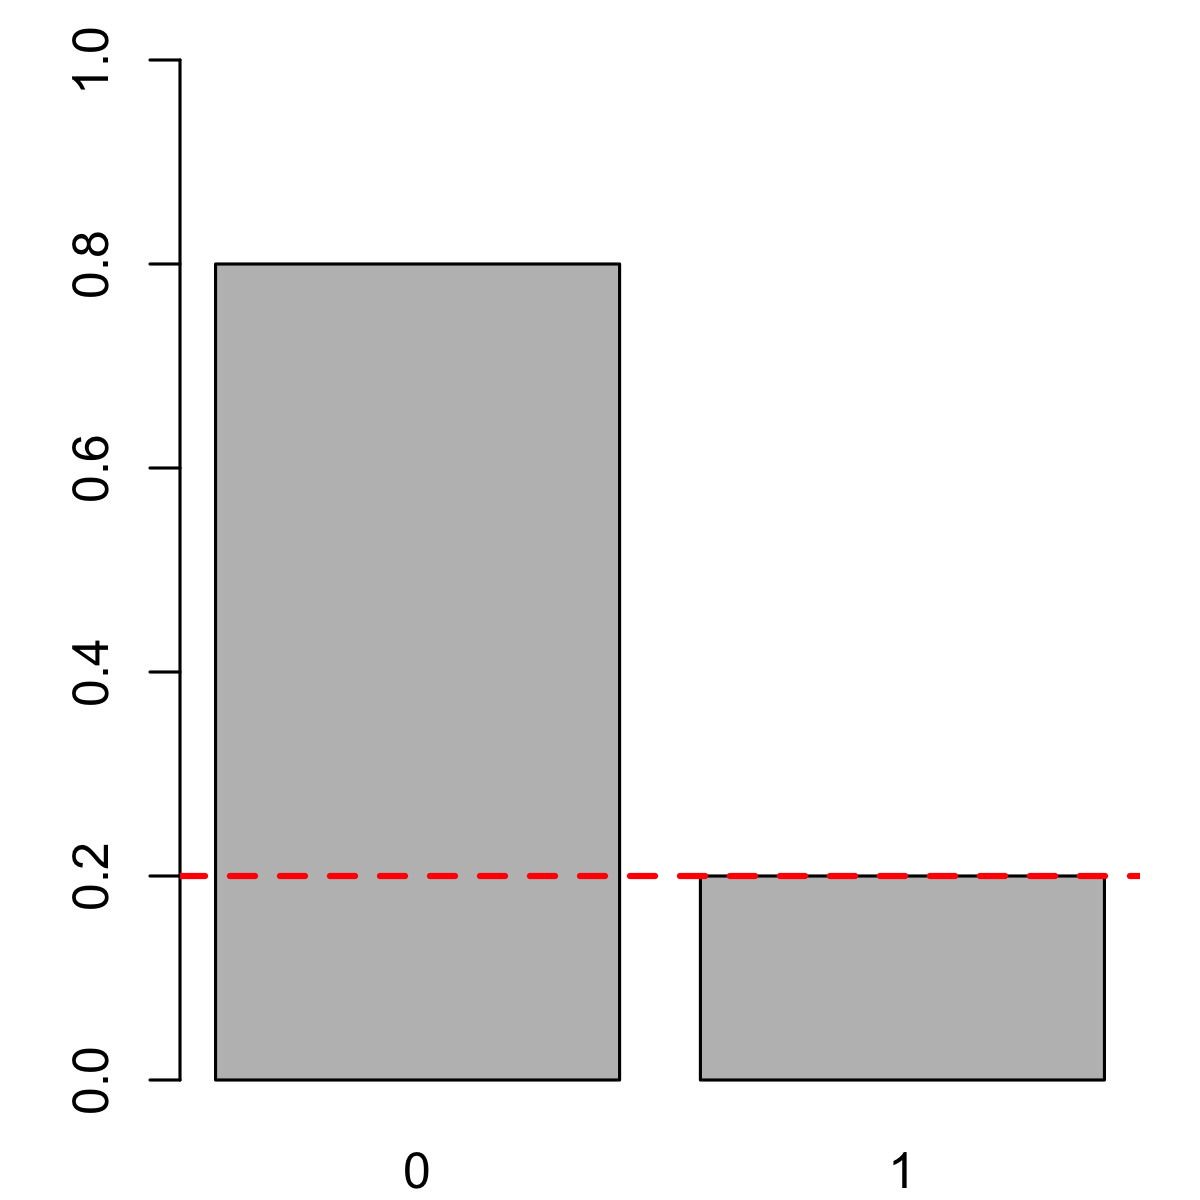
\includegraphics[width=0.3\textwidth]{img/l01-figure2c-bernoulli-0-2.png}
\end{center}

The \textbf{categorical distribution} is a generalization of the Bernoulli distribution to an outcome with more than two levels. The categorical distribution looks like this:
$$ p(x|\phi_1, \dots, \phi_K) = \phi_1^{\mathbb{I}(x=1)} \phi_2^{\mathbb{I}(x=2)} \cdots \phi_K^{\mathbb{I}(x=K)} $$
where $\sum_{k=1}^K \phi_k = 1$. The term $\mathbb{I}(x=j)$ is an \textbf{indicator}. It equals 1 if $x=j$ and 0 otherwise. For example, $\mathbb{I}(x=2)$ is 1 if $x=2$ and 0 otherwise. 

\begin{question}{}
List 5 random variables from medicine or biology that should follow Bernoulli distributions.
\end{question}


\section{Binomial Distribution \label{sect:binomial}}

The \textbf{binomial distribution} models the number of positive outcomes, $x$, out of $n$ independent\footnote{The word \textbf{independent} just means that the outcome of one trial does not influence the outcome of any other trial.} Bernoulli trials, each of which is positive with probability $\mu$. This distribution has the following properties, with $x \in \{0, \dots, n\}$:
$$ p(x|n,\mu) = {n\choose x} \mu^x (1 - \mu) ^ {n-x} \qquad E[x| \mu] = n \mu \qquad \text{var}(x | \mu) = n \mu (1 - \mu) $$
where the notation ${n \choose x}$ is defined as:
$$ {n \choose x} = \frac{n!}{x!(n-x)!}. $$
This notation denotes the number of ways it is possible to choose $x$ things out of a group of $n$ things, where the ordering doesn't matter. The exclamation point denotes the \textbf{factorial function}: $x! = x(x-1)(x-2)\cdots(2)(1)$. 

The shape of the binomial distribution is governed by the values of $n$ and $\mu$. Here, we vary $n$ but keep $\mu$ constant at $0.5$:
\begin{center}
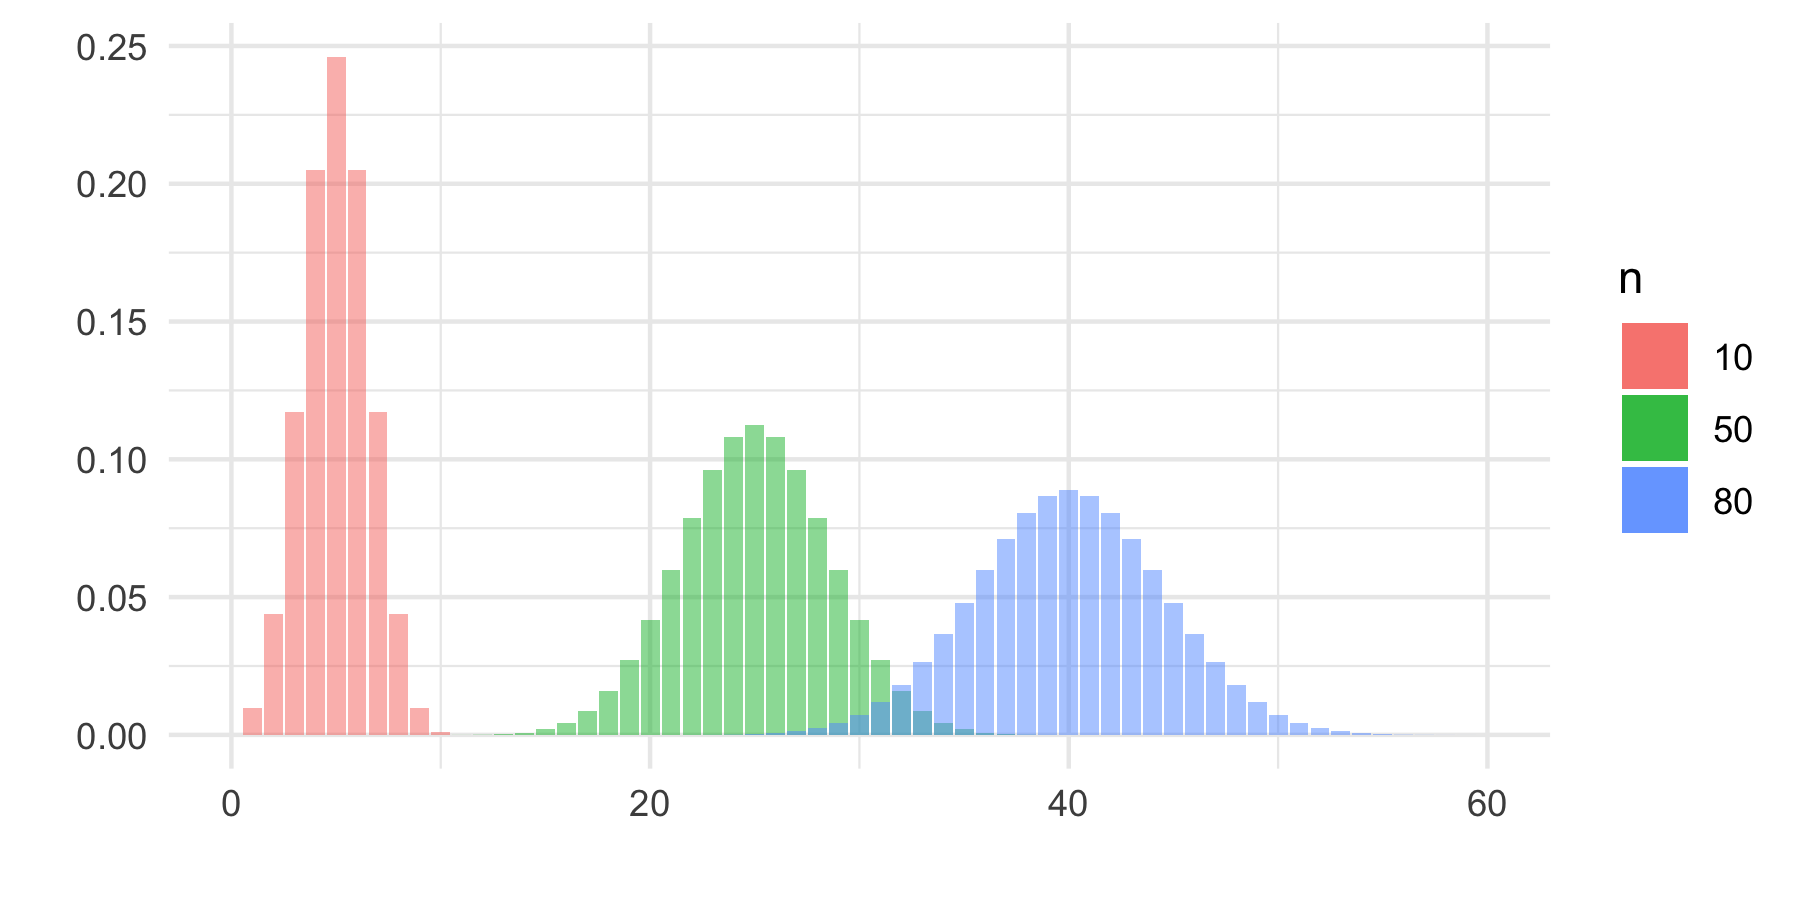
\includegraphics[width=0.9\textwidth]{img/l01-figure3-binom-n-change.png}
\end{center}
And here we vary $\mu$ but keep $n$ constant at $50$:
\begin{center}
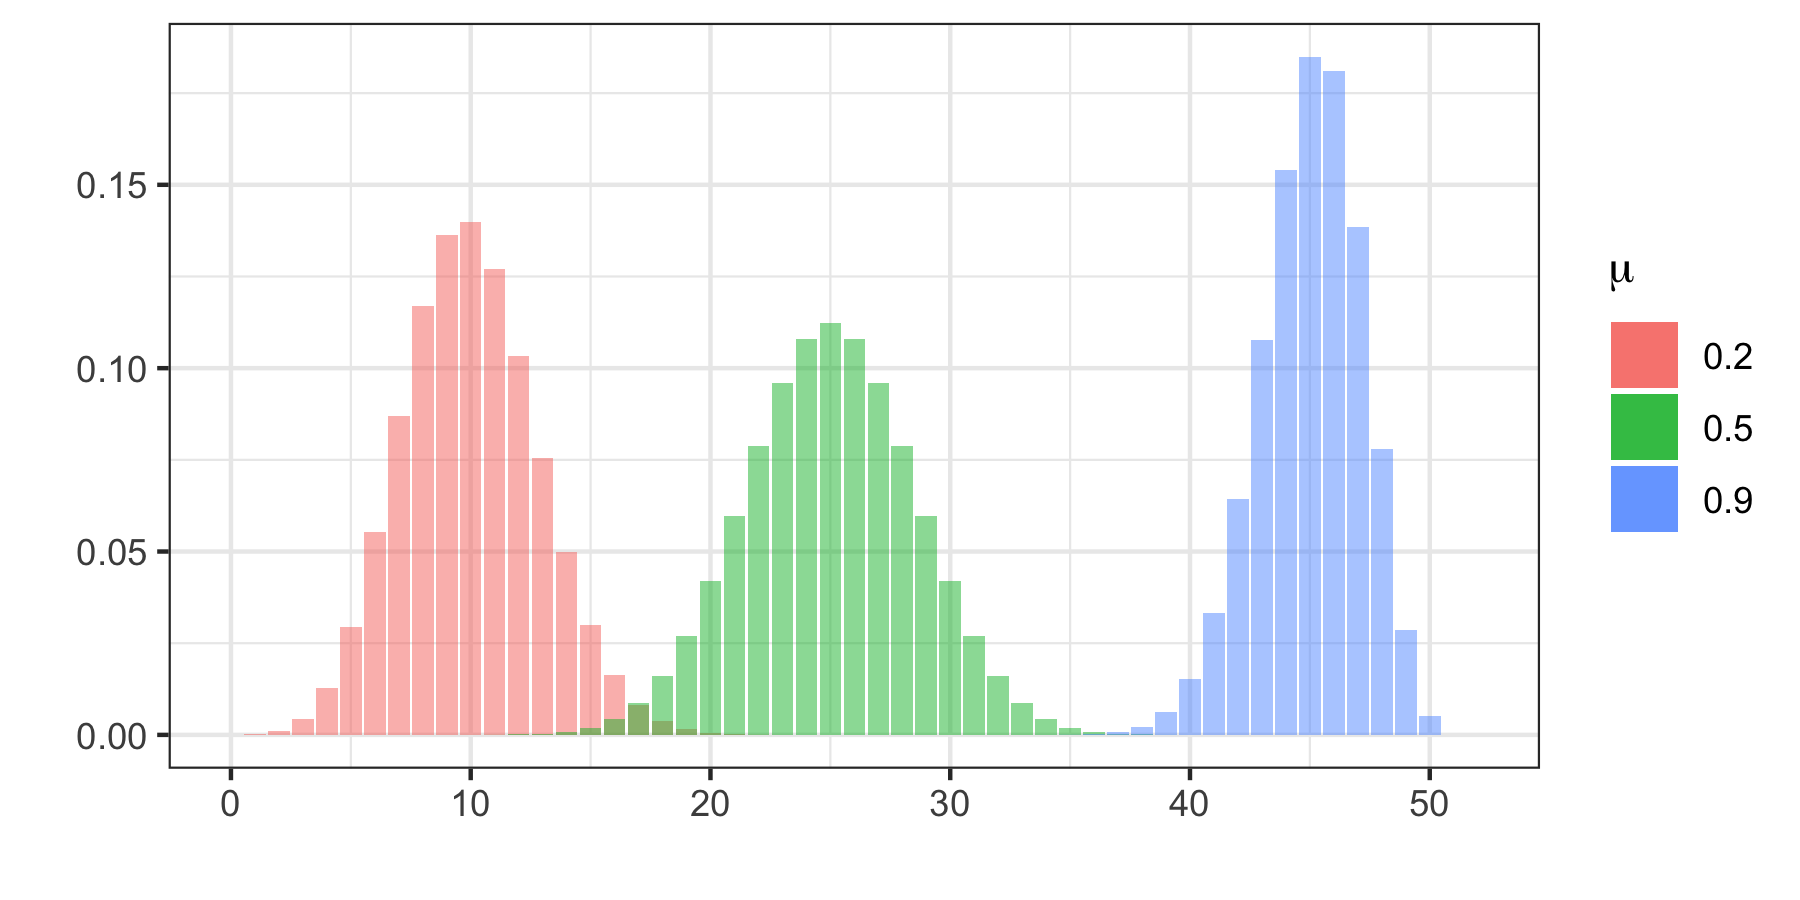
\includegraphics[width=0.9\textwidth]{img/l01-figure4-binom-p-change.png}
\end{center}

\begin{question}{question:binomialex}
List 5 random variables from medicine or biology that should follow binomial distributions.
\end{question}


\section{Poisson Distribution \label{sect:poisson}}

The \textbf{Poisson distribution} is a probability distribution that is often used to model discrete quantitative data, such as counts. It has the following properties:
$$ p(x | \lambda) = \frac{e^{-\lambda} \lambda^x}{x!} \qquad E[x|\lambda] = \lambda \qquad \text{var}(x|\lambda) = \lambda $$
where $x \in \left\{0, 1, 2, \dots \right\}$. Below are four examples of Poisson distributions. If events of a particular type occur continuously and independently at a constant rate (\textbf{Poisson process}), the number of events within a time window of fixed width will be distributed according to the Poisson distribution, with rate parameter $\lambda$ proportional to the width of the window.

Situations where the population size, $n$, is large, the probability of an individual event, $p$, is small, but the expected number of events, $np$, is moderate (say five or more) can generally be modeled using a Poisson distribution with $\lambda = np$. 

\begin{center}
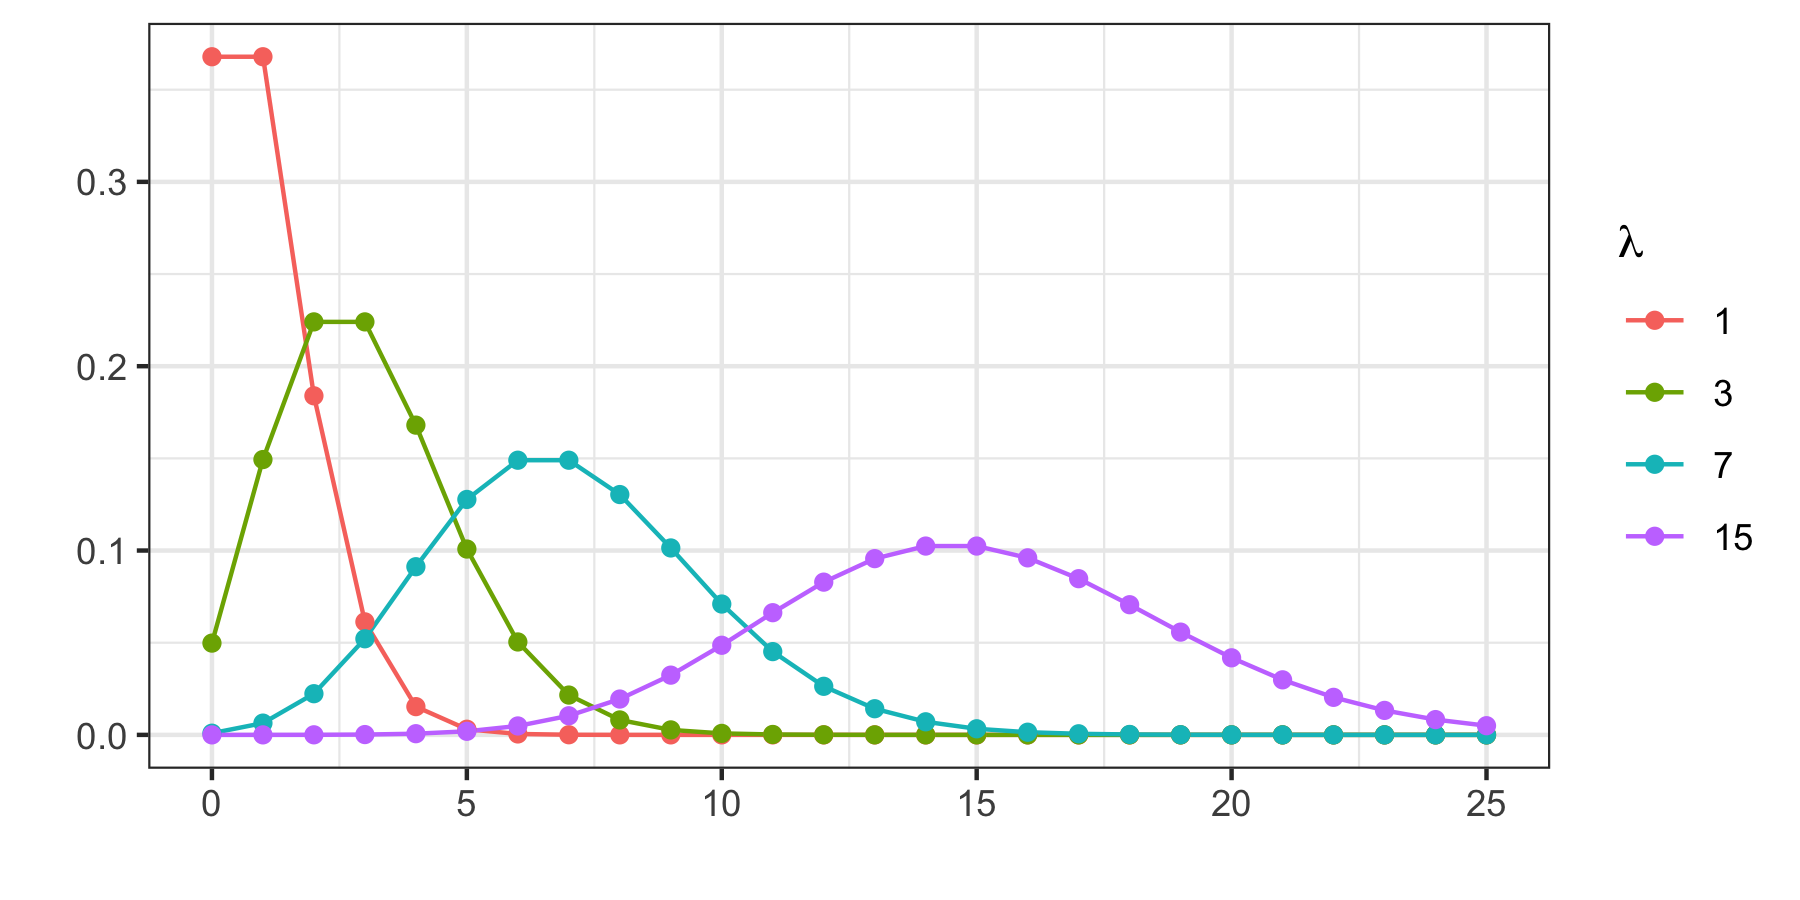
\includegraphics[width=0.9\textwidth]{img/l01-figure3a-poisson-lambda-change.png}
\end{center}

\begin{question}{question:poissonex}
List 5 random variables from medicine or biology that should follow Poisson distributions.
\end{question}


\section{Geometric \label{sect:geometric}}

The \textbf{geometric distribution} models the number of failures in a sequence of Bernoulli trials before the first success. It has the following properties:
$$ p(x|\mu) = (1-\mu)^x \mu \qquad E[x|\mu] = \frac{1-\mu}{\mu} \qquad \text{var}(x|\mu) = \frac{1-\mu}{\mu^2}  $$
for $x \in \left\{0, 1, 2, \dots \right\}$, where $\mu$ refers to the probability (in the Bernoulli trial) that the trial is a success. Some examples of geometric distributions with different $\mu$ are shown below: 
\begin{center}
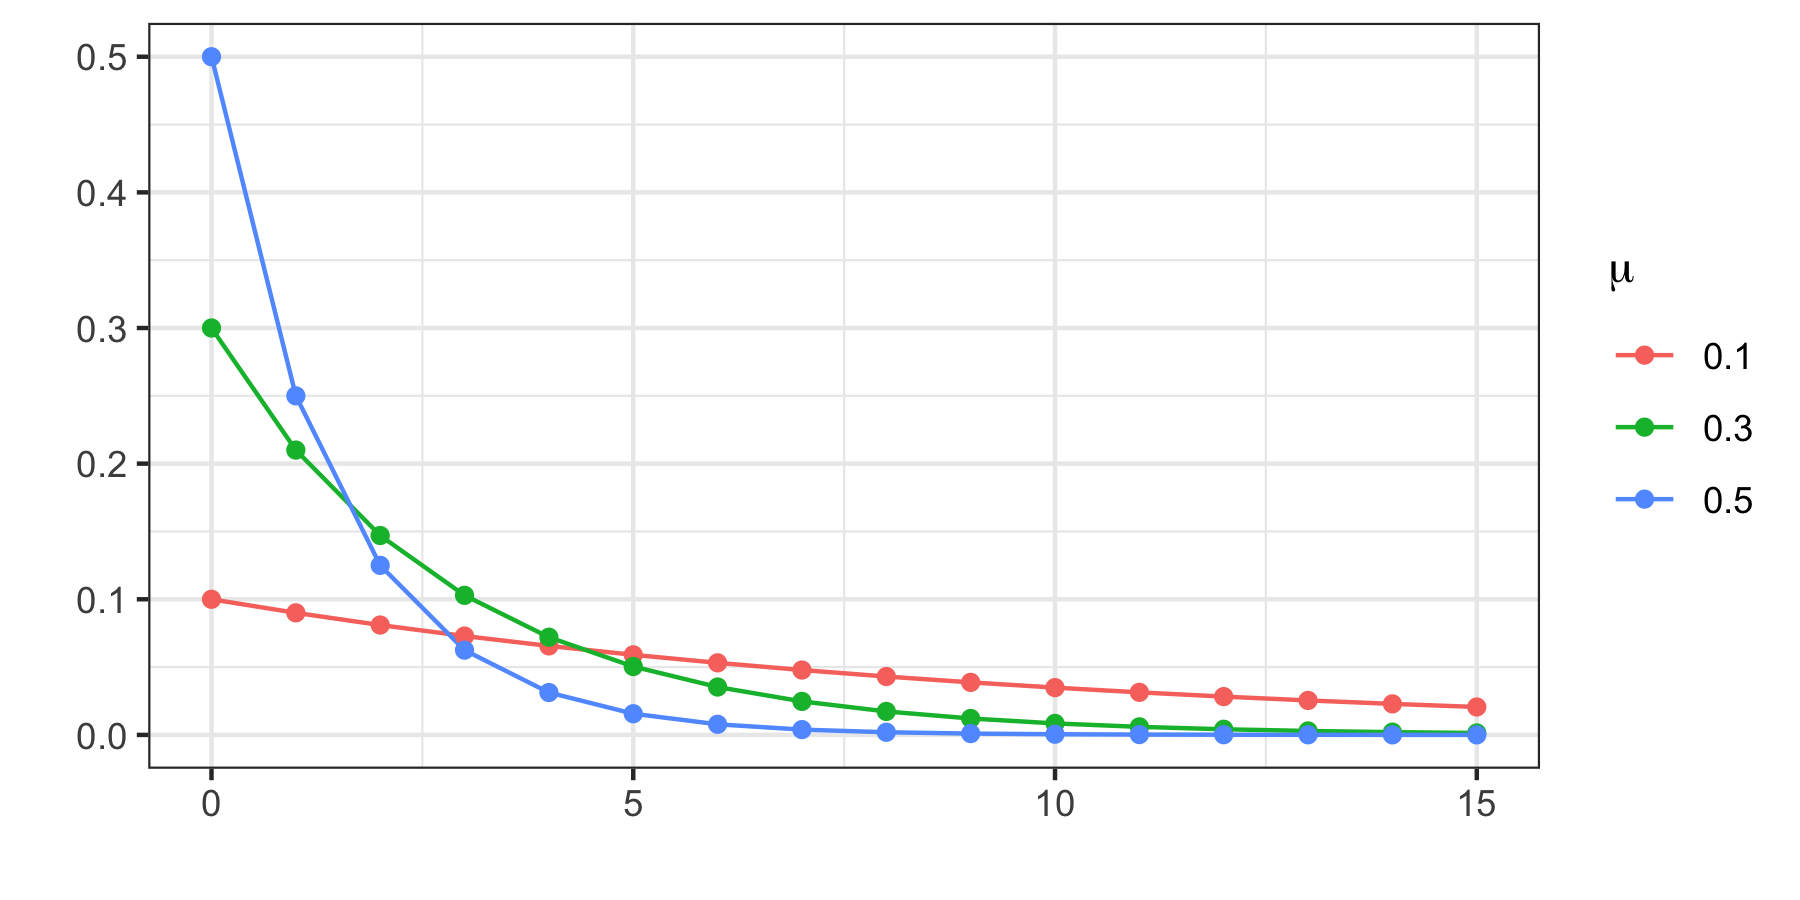
\includegraphics[width=0.9\textwidth]{img/l01-figure4-geometric-mu-change.png}
\end{center}

\begin{question}{question:geometricex}
List 5 random variables from medicine or biology that should follow Poisson distributions.
\end{question}


\section{Exponential \label{sect:exponential}}

The \textbf{exponential distribution} is a continuous probability distribution that models waiting times between events that happen independently and continuously at a constant rate (Poisson process), as well as many other random variables\footnote{For example, in an epidemiologic model of an infectious process like COVID-19 community spread, exponential waiting times are often used to model transitions between the susceptible, exposed, infectious, and recovered compartments in the model.}. It has the following properties:
$$ p(x|\lambda) = \lambda e^{-\lambda x} \qquad E[x|\lambda] = \frac{1}{\lambda} \qquad \text{var}(x|\lambda) = \frac{1}{\lambda^2} $$
where $x \in \mathbb{R}^+$ ($x$ is a positive real number, or zero). The exponential distribution is the continuous analogue of the geometric distribution. It is memoryless, which means that the distribution of a waiting time until an event does not depend on how much time has elapsed already.

Here are some different exponential distributions. Compare them to the geometric distribution, above.
\begin{center}
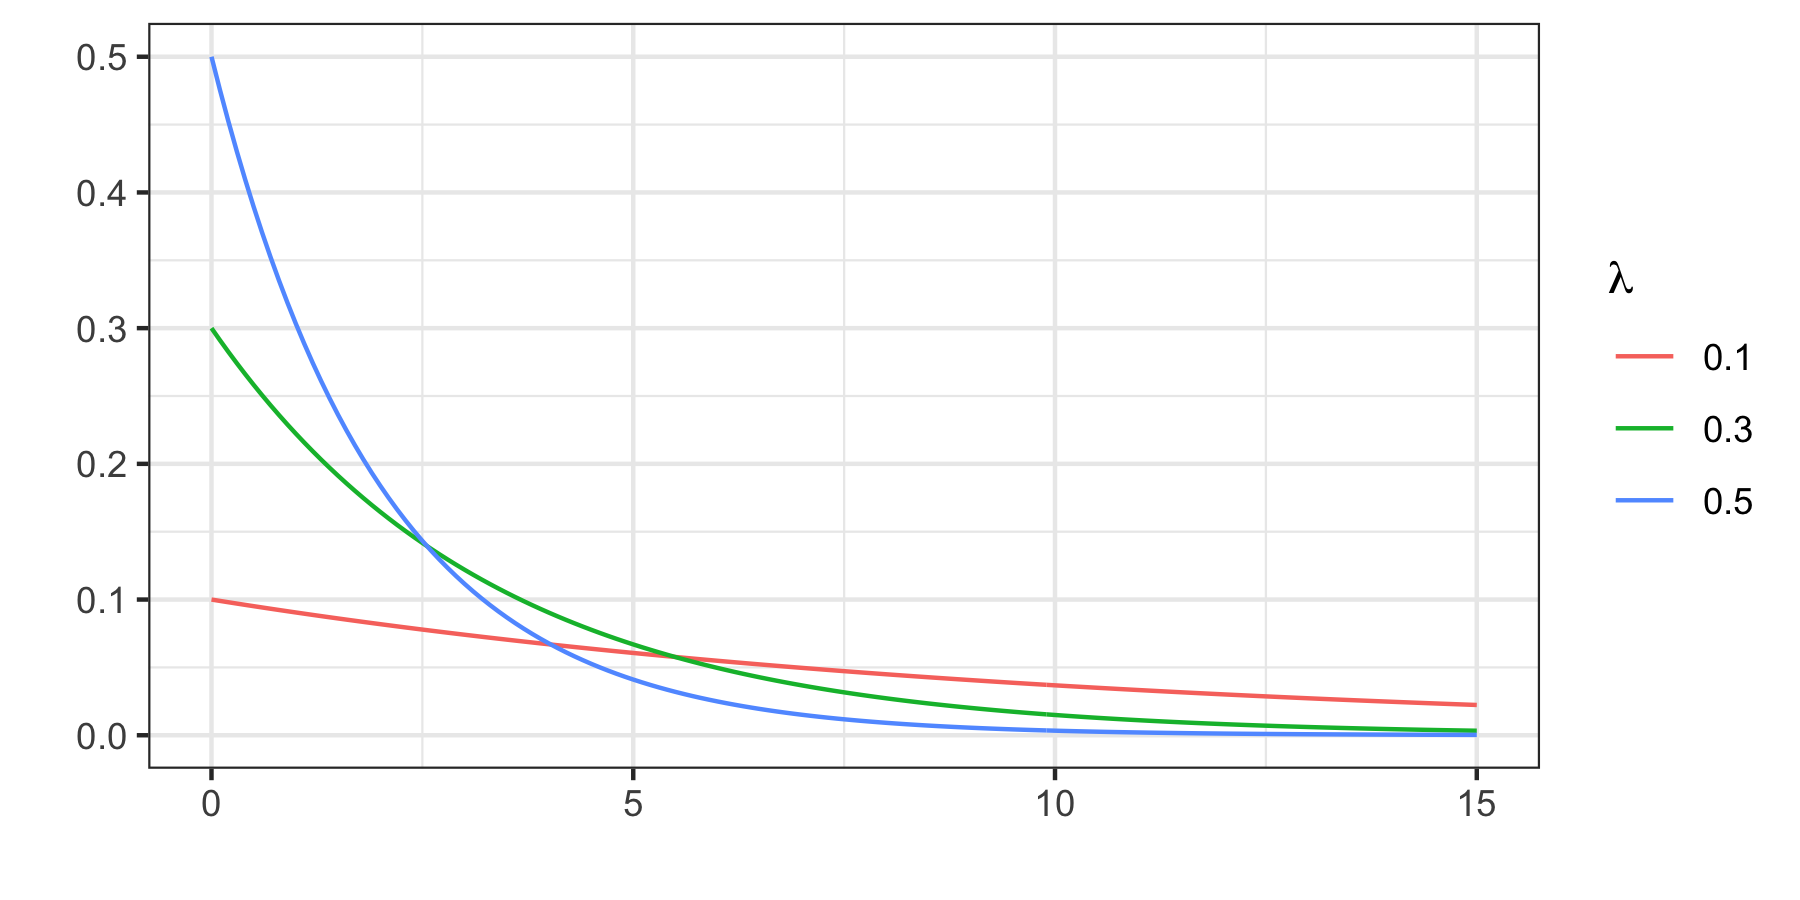
\includegraphics[width=0.9\textwidth]{img/l01-figure5-exponential-lambda-change.png}
\end{center}

\begin{question}{question:exponentialex}
List 5 random variables from medicine or biology that should follow exponential distributions.
\end{question}


\section{Chi-Squared Distribution}

How this distribution arises:
\begin{enumerate}
\item If $Z \sim \mathcal{N}(0, 1)$, the distribution of $U = Z^2$ is called the chi-squared distribution with one degree of freedom.
\item If $U_1, U_2, \dots, U_k$ are independent $\chi_1^2$ random variables, their sum,
$ V = \sum_{i=1}^k U_i $
follows $\chi_k^2$, a chi-squared distribution with $k$ degrees of freedom.
\end{enumerate}

You'll often see the chi-squared distribution used as the sampling distribution for the sample variance in a variety of statistical hypothesis tests. It looks like this:
\begin{center}
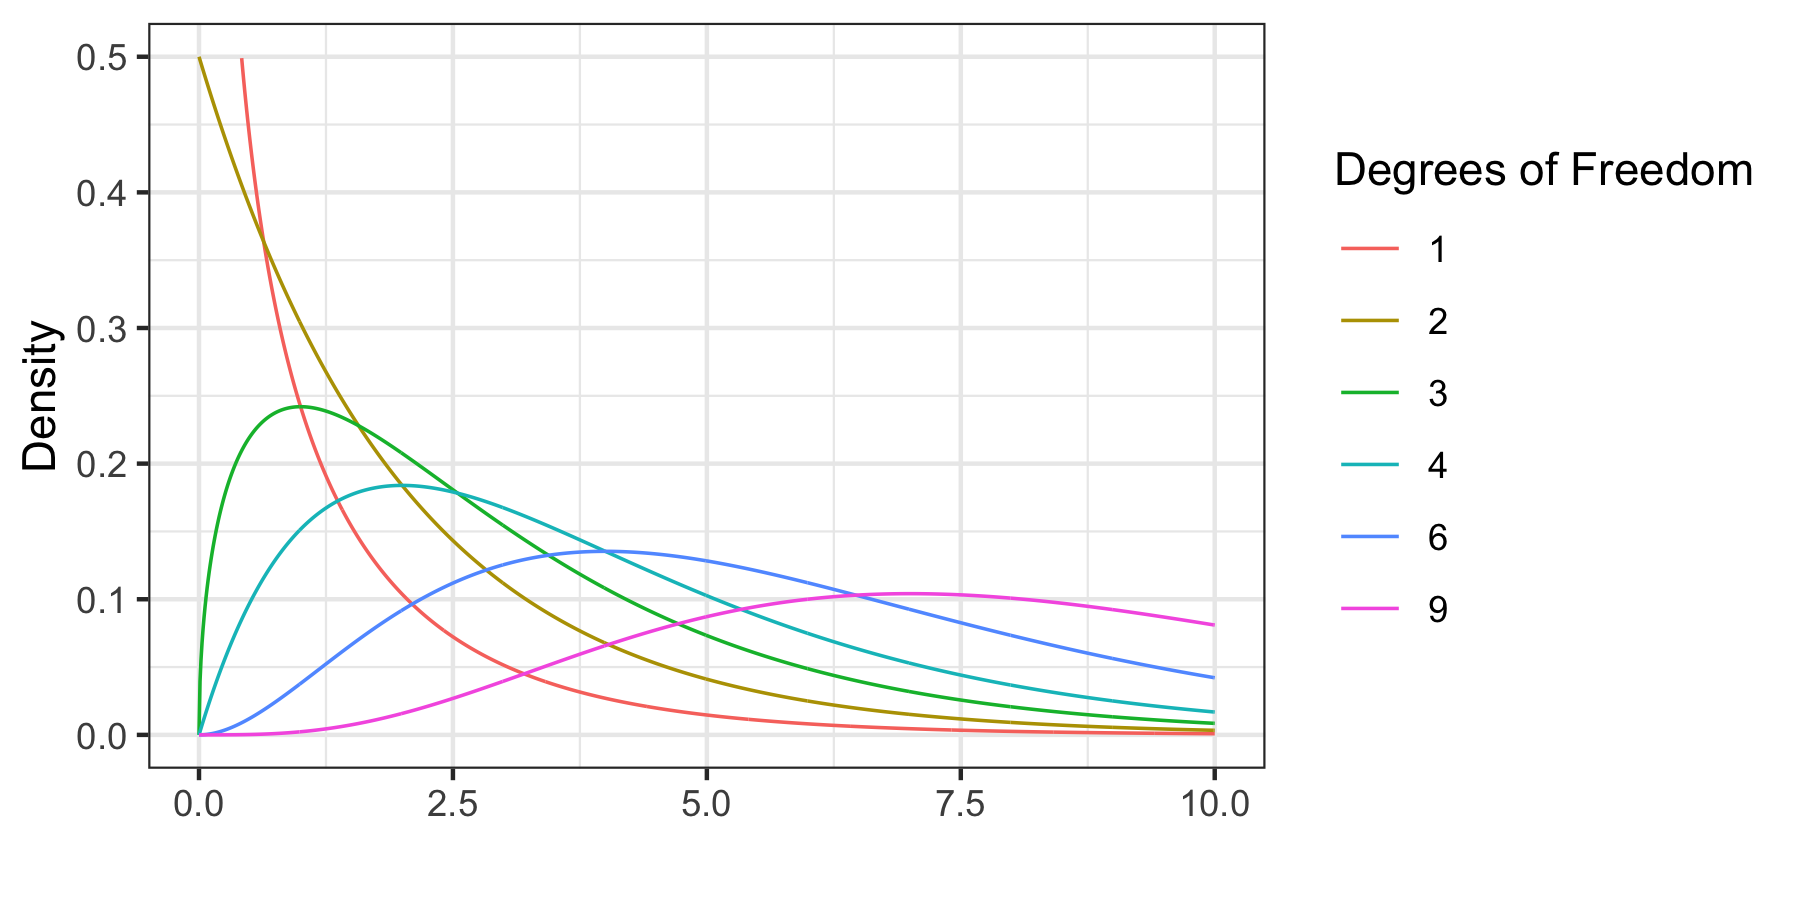
\includegraphics[width=0.9\textwidth]{img/hyp-example-chisq-distribution.png}
\end{center}

The parameter $k$, the \textbf{degrees of freedom}, controls the shape of the chi-squared distribution. The actual formula for the chi-squared distribution looks a bit intimidating, but I'm including it here so you can compare it to the other distributions we've seen:
$$ p(x|k) = \frac{1}{2^{k/2} \Gamma(k/2)} x^{k/2 - 1} e^{-x/2} $$
$$ E[x | k] = k \qquad \text{var}(x | k) = 2k $$ 
The gamma function shown in the denominator of the probability density,
$$ \Gamma(z) = \int_0^{\infty} x^{z-1} e^{-x} dx, $$
is a generalization of the factorial function to complex numbers. For any positive integer $n$, $\Gamma(n) = (n-1)!$. 

\section{Student's T Distribution}

If $Z \sim \mathcal{N}(0, 1)$ and $U \sim \chi_k^2$ and $Z$ and $U$ are independent, 
$$ T = \frac{Z}{\sqrt{U/k}} \sim t_k $$
or in words, the statistic $T$ follows a $t$-distribution with $k$ degrees of freedom. The T distribution plays an important role in a family of statistical hypothesis tests called T-tests. 

\begin{center}
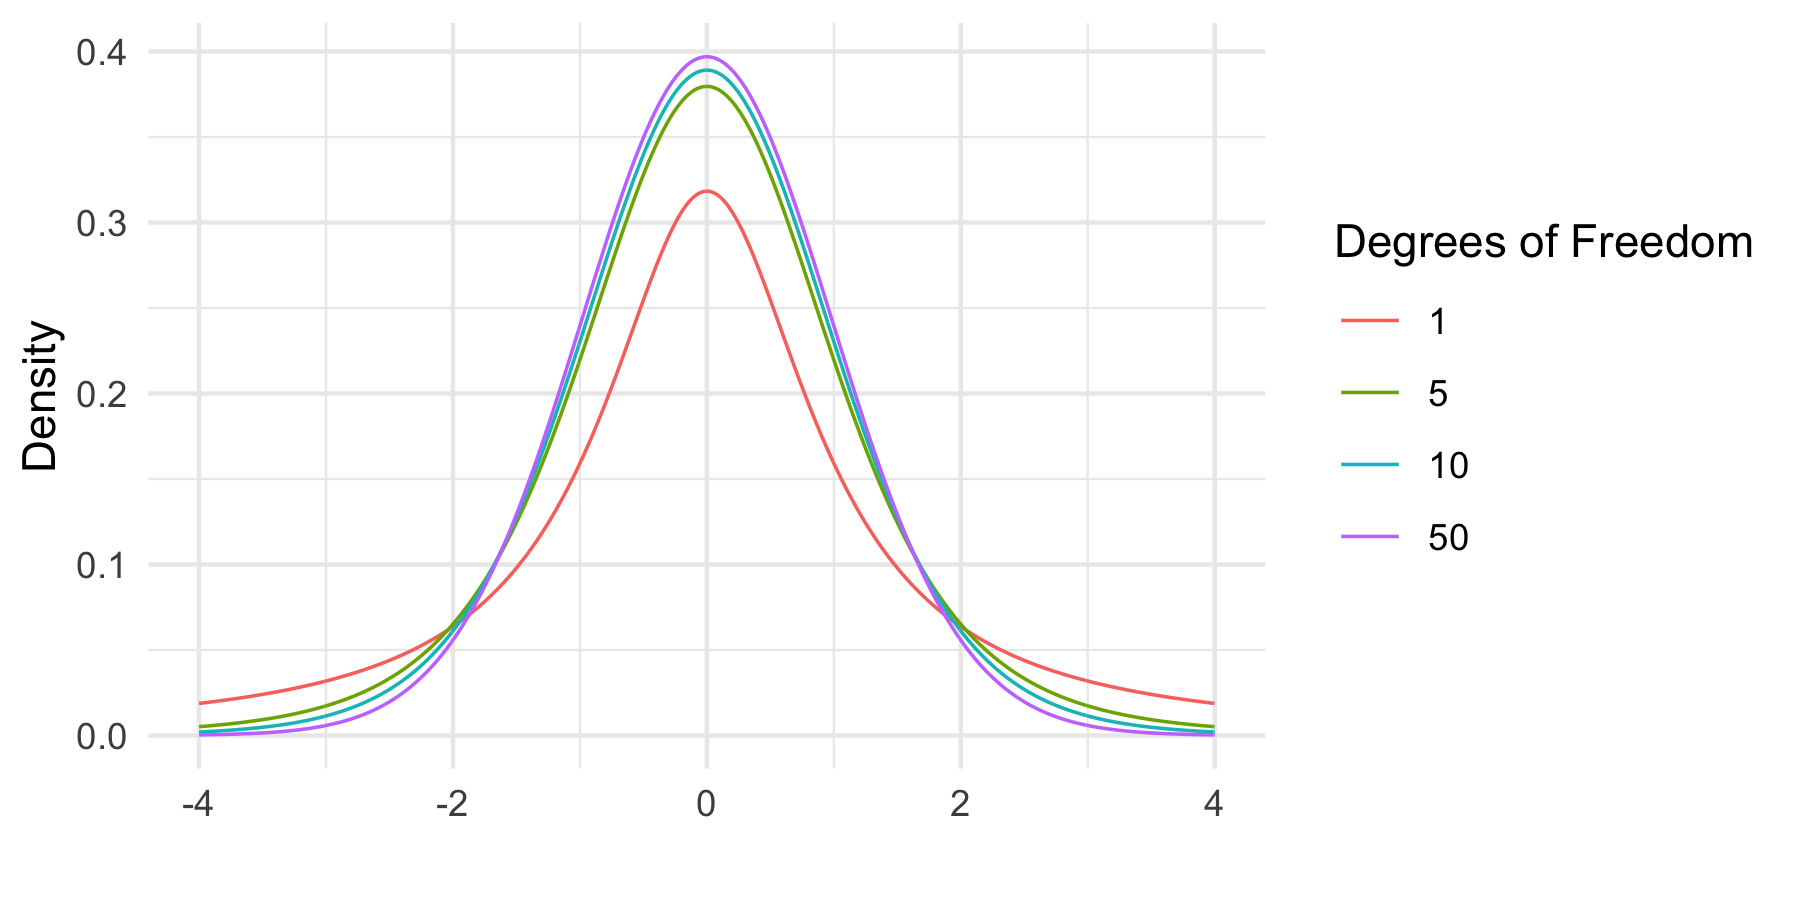
\includegraphics[width=0.9\textwidth]{img/hyp-example-t-distribution.png}
\end{center}

Again, the functional form of the T distribution is a bit intimidating, but I'm including it for completeness:

$$ p(x|k) = \frac{\Gamma \left(\frac{k+1}{2} \right)} {\sqrt{k\pi}\,\Gamma \left(\frac{k}{2} \right)} \left(1+\frac{x^2}{k} \right)^{-\frac{k+1}{2}} $$
$$ E[x|k] = 0~~\text{ for }k>1; \text{ otherwise undefined} $$
$$ \text{var}(x|k) = \left\{ \begin{array}{cl} \frac{k}{k-2} & k>2 \\
                                               \infty & 1 < k \leq 2 \\
                                               \text{undefined} & \text{otherwise} \end{array} \right. $$

\section{F Distribution}

If $U$ and $V$ are independent $\chi^2$ random variables with $m$ and $n$ degrees of freedom,
$$ W = \frac{U/m}{V/n} \sim F_{m, n} $$
or in words, the statistic $W$ follows an $F$ distribution with $m$ and $n$ degrees of freedom. I'm not writing out the functional form of the F distribution here because it's too awful-looking, but graphically it looks like this:
\begin{center}
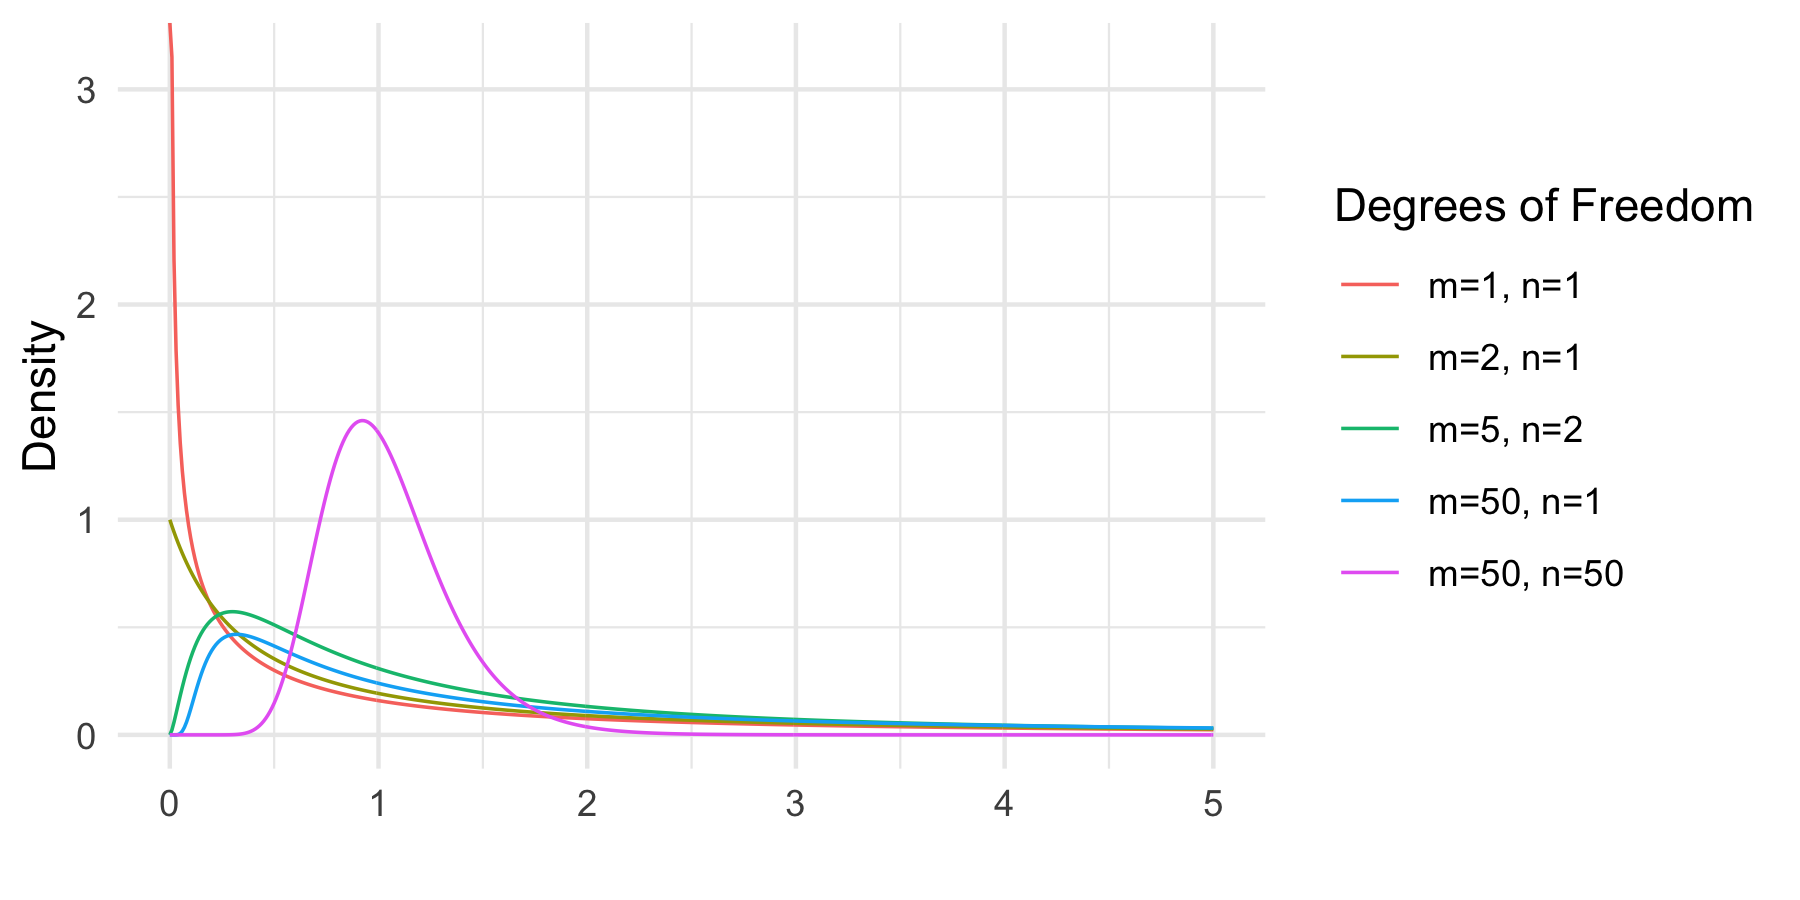
\includegraphics[width=0.9\textwidth]{img/hyp-example-f-distribution.png}
\end{center}

Note that if $T \sim t_k$, then $T^2 \sim F_{1,k}$. The $F$-distribution plays an important role in a class of statistical analysis techniques called \textbf{ANalysis Of VAriance}, or \textbf{ANOVA}.

\vspace{2mm}

\begin{question}{question:likexamples}
For each of the following experimental conditions, which distribution (from those listed above) provides the best model for how the data $x^{(1)},\dots,x^{(n)}$ are generated?
    \begin{enumerate}
    \item[(a)] You are observing several patients' skin in a clinical study to see how long it takes them to develop a rash. You take a picture each day. Let $x^{(i)}$ be the number of days of \emph{no rash} before the rash occurs.

\begin{center}{\small
\begin{tabular}{cc}
\toprule
Patient ID ($i$) & $x^{(i)}$ \\
\midrule
1 & 4 \\
2 & 1 \\
3 & 0 \\
4 & 2 \\
5 & 2 \\
6 & 4 \\
7 & 3 \\
8 & 1 \\
9 & 0 \\
10 & 1 \\
\end{tabular}}
\end{center}

    \item[(b)] Same situation as above except that instead of taking a picture each day, the patient texts you at the moment he/she observes a rash. The data look like this, where $x^{(i)}$ is the time (in days) at which patient $i$ develops a rash: 

\begin{center}{\small
\begin{tabular}{cc}
\toprule
Patient ID ($i$) & $x^{(i)}$ \\
\midrule
1 & 2.25 \\
2 & 3.43\\
3 & 0.68\\
4 & 0.04\\
5 & 3.78\\
6 & 5.65\\
7 & 2.88\\
8 & 3.88\\
9 & 2.83\\
10 & 1.87\\
\end{tabular}}
\end{center}
 
    \item[(c)] Imagine you are Ladislaus Bortkiewicz, and you are modeling the number of persons killed by mule or horse kicks in the Prussian army per year. You have data from the late 1800s over the course of 20 years. Let $x^{(i)}$ be the number of people killed in year $i$.
        
\begin{center}{\small
\begin{tabular}{cc|cc}
\toprule
Year ($i$) & $x^{(i)}$ & Year ($i$) & $x^{(i)}$ \\
\midrule
1 & 8 & 11 & 9 \\
2 & 10 & 12 & 7 \\
3 & 5 & 13 & 10 \\
4 & 3 & 14 & 12 \\
5 & 10 & 15 & 8 \\
6 & 8 & 16 & 7 \\
7 & 7 & 17 & 8 \\
8 & 2 & 18 & 8 \\
9 & 6 & 19 & 10 \\
10 & 11 & 20 & 7 \\
\end{tabular}}
\end{center}
    
    \item[(d)] Every year, $10$ scientists go to the same geographic area (same Lyme prevalence) and they each collect $40$ ticks. They test each tick for Lyme disease and record the number of ticks that have Lyme. Let $x^{(i)}$ be the number of ticks with Lyme in the $i$th scientist's bunch.
        
\begin{center}{\small
\begin{tabular}{cc}
\toprule
Scientist ID ($i$) & $x^{(i)}$ \\
\midrule
1 & 8 \\
2 & 9 \\
3 & 14 \\
4 & 15 \\
5 & 12 \\
6 & 7 \\
7 & 6 \\
8 & 8 \\
9 & 8 \\
10 & 14 \\
\end{tabular}}
\end{center}
    
    \item[(e)] You have waist circumference data on 1045 men aged 70 and above (see Dey's 2002 paper in the Journal of the American Geriatric Society). It looks like this:
    
\begin{center}
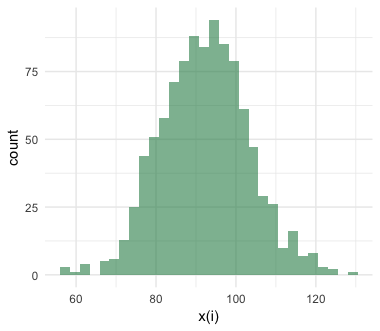
\includegraphics[width=0.5\textwidth]{img/l01-problem5.png}
\end{center}

    \end{enumerate}
\end{question}


\chapter{Maximum Likelihood Estimation \label{chapter:mlebasics}}

Maximum likelihood (ML) is the most widely used technique for fitting data to probability distributions. In this technique, we choose parameter value(s) for a probability distribution that maximize the probability, or \textbf{likelihood}\index{likelihood}, that it generated our observed data.

\section{Likelihood}

If we draw independent\footnote{Independent sampling just means that the values of different samples do not depend on each other.} samples from the same distribution, $p(x|\theta)$, the {\bf joint density function} for all $n$ observations is:
$$ p(x^{(1)}, x^{(2)}, \dots, x^{(n)}|\theta) = \prod_{i=1}^n p(x^{(i)}|\theta). $$
Since the data are known but the parameter(s) $\theta$ are unknown, we typically view this thing as a function of $\theta$:
$$ \mathcal{L}(\theta) = \prod_{i=1}^n p(x^{(i)}|\theta). $$

The higher the joint probability of the data (the more ``likely'' the data are) given $\theta$, the higher the value of this function. We call $\mathcal{L}(\theta)$ the \textbf{likelihood}\footnote{The distributions we have discussed so far are from a broad family of probability distributions called the {\bf exponential family}. One of the properties of this family is that the log-likelihood is concave. Practically speaking, this means that if we maximize the log-likelihood by setting derivatives equal to zero, we are guaranteed to (a) get only one solution, and (b) find a maximum (not a minimum or an inflection point).}. Frequently we will want to use the logarithm of the likelihood, which we call the \textbf{log-likelihood}, because it has some nice properties, including allowing us to work with sums instead of products\footnote{Note that if the function $f(z)$ has a maximum at $z'$, the function $\log f(z)$ will also have a maximum at $z'$, because the logarithmic function is monotonically increasing. So we will get the same estimate either way.}:
$$ \log \mathcal{L}(\theta) = \sum_{i=1}^n \log p(x^{(i)}|\theta). $$

In {\bf maximum likelihood estimation}\index{maximum likelihood estimation}, we seek to find the $\theta$ for which the likelihood (or log-likelihood) is maximized. We do this by taking derivatives of the log-likelihood with respect to the various parameters and setting them equal to zero. The best-fit parameter estimates obtained in this way are called the \textbf{maximum likelihood estimates (MLEs)}. 

We will now go through a bunch of examples of how to find the MLEs of the probability distributions we saw in Chapter~\ref{chapter:probabilitydistributions}. 

\section{Bernoulli MLE}

First, write down the log-likelihood.
\begin{align*}
\log \mathcal{L}(\mu) &= \sum_{i=1}^n \log p(x^{(i)}|\mu) \\
&= \sum_{i=1}^n \log \left( \mu^{x^{(i)}}(1-\mu)^{1-x^{(i)}} \right) \\
&= \sum_{i=1}^n \left[ x^{(i)} \log(\mu) + (1-x^{(i)}) \log(1-\mu) \right] \end{align*}
Now take the derivative of the log-likelihood with respect to $\mu$:
\begin{align*}
\frac{d}{d \mu} \log \mathcal{L}(\mu) = \sum_{i=1}^n \left[ \frac{x^{(i)}}{\mu} - \frac{1-x^{(i)}}{1-\mu} \right]
\end{align*}
Set this equal to zero and solve for $\hat{\mu}$ (the maximum likelihood estimate of $\mu$):
\begin{align*} \sum_{i=1}^n \left[ \frac{x^{(i)}}{\hat{\mu}} - \frac{1-x^{(i)}}{1-\hat{\mu}} \right] = 0 & \implies (1 - \hat{\mu}) \sum_{i=1}^n x^{(i)} = \hat{\mu} \sum_{i=1}^n (1 - x^{(i)}) \\
& \implies \boxed{\hat{\mu} = \frac{1}{n} \sum_{i=1}^n x^{(i)}} \end{align*}

\section{Binomial MLE}

Here we assume $m$ (the number of trials) is a known quantity. First, write down the log-likelihood.
\begin{align*}
\log \mathcal{L}(\mu) &= \sum_{i=1}^n \log p(x^{(i)}|m,\mu) \\
&= \sum_{i=1}^n \log \left[ {m\choose x} \mu^x (1 - \mu) ^ {m-x} \right] \\
&= \sum_{i=1}^n \left[\log(m!) - \log(x!) - \log((m-x)!) + x^{(i)} \log(\mu) + (m-x^{(i)}) \log(1-\mu) \right] \end{align*}
Now take the derivative of the log-likelihood with respect to $\mu$:
\begin{align*}
\frac{d}{d \mu} \log \mathcal{L}(\mu) = \sum_{i=1}^n \left[ \frac{x^{(i)}}{\mu} - \frac{m-x^{(i)}}{1-\mu} \right]
\end{align*}
Set this equal to zero and solve for $\hat{\mu}$ (the maximum likelihood estimate of $\mu$):
\begin{align*} \sum_{i=1}^n \left[ \frac{x^{(i)}}{\hat{\mu}} - \frac{m-x^{(i)}}{1-\hat{\mu}} \right] = 0 & \implies (1 - \hat{\mu}) \sum_{i=1}^n x^{(i)} = \hat{\mu} \sum_{i=1}^n (m - x^{(i)}) \\
& \implies \boxed{\hat{\mu} = \frac{1}{nm} \sum_{i=1}^n x^{(i)}} \end{align*}

\section{Normal MLE}

First, write down the log-likelihood.
\begin{align*}
\log \mathcal{L}(\mu, \sigma) &= \sum_{i=1}^n \log p(x^{(i)}|\mu, \sigma) \\
&= \sum_{i=1}^n \log \left( \frac{1}{\sqrt{2 \pi \sigma^2}} e^{-\frac{(x^{(i)}-\mu)^2}{2 \sigma^2}} \right) \\
&= -\frac{n}{2} \log (2 \pi) - \frac{n}{2} \log \sigma^2 - \frac{1}{2 \sigma^2} \sum_{i=1}^n \left( x^{(i)} - \mu \right)^2 \\
\end{align*}
To find the MLE for $\mu$, take the derivative of the log-likelihood with respect to $\mu$:
\begin{align*}
\frac{\partial}{\partial \mu} \log \mathcal{L}(\mu, \sigma) = \frac{1}{\sigma^2} \sum_{i=1}^n \left( x^{(i)} - \mu \right)
\end{align*}
Set this equal to zero and solve for $\hat{\mu}$ (the maximum likelihood estimate of $\mu$):
\begin{align*} \frac{1}{\sigma^2} \sum_{i=1}^n \left( x^{(i)} - \mu \right) = 0 & \implies \boxed{\hat{\mu} = \frac{1}{n} \sum_{i=1}^n x^{(i)}} \end{align*}
To find the MLE for $\sigma$, take the derivative of the log-likelihood with respect to $\sigma$:
\begin{align*} \frac{\partial}{\partial \sigma} \log \mathcal{L}(\mu, \sigma) &= -\frac{n}{\sigma} + \frac{1}{\sigma^3} \sum_{i=1}^n \left( x^{(i)} - \mu \right)^2
\end{align*}
Set this equal to zero and solve for $\hat{\sigma}$ (the maximum likelihood estimate of $\sigma$)\footnote{One detail: it turns out this estimate is biased because it depends on the MLE for $\mu$. An unbiased version has $n-1$ in the denominator instead of $n$. The effect of this is minimal unless $n$ is really small.}. Note that the answer depends on our previous MLE of $\mu$:
\begin{align*}
-\frac{n}{\hat{\sigma}} + \frac{1}{\hat{\sigma}^3} \sum_{i=1}^n \left( x^{(i)} - \mu \right)^2 = 0  & \implies \boxed{\hat{\sigma} = \sqrt{\frac{1}{n} \sum_{i=1}^n \left( x^{(i)} - \hat{\mu} \right)^2}}
\end{align*}

\section{Poisson MLE}

First, write down the log-likelihood.
\begin{align*}
\log \mathcal{L}(\lambda) &= \sum_{i=1}^n \log p(x^{(i)}|\lambda) \\
&= \sum_{i=1}^n \log \left( \frac{e^{-\lambda} \lambda^{x^{(i)}}}{x^{(i)}!} \right) \\
&= \sum_{i=1}^n \left[ -\lambda + x^{(i)} \log(\lambda) - \log(x^{(i)}!) \right] \end{align*}
Now take the derivative of the log-likelihood with respect to $\lambda$:
\begin{align*}
\frac{d}{d \lambda} \log \mathcal{L}(\lambda) = \sum_{i=1}^n \left[ -1 + \frac{x^{(i)}}{\lambda} \right]
\end{align*}
Set this equal to zero and solve for $\hat{\lambda}$ (the maximum likelihood estimate of $\lambda$):
\begin{align*} \sum_{i=1}^n \left[ -1 + \frac{x^{(i)}}{\hat{\lambda}} \right] = 0 & \implies \boxed{\hat{\lambda} = \frac{1}{n} \sum_{i=1}^n x^{(i)}} \end{align*}

\section{Geometric MLE}

First, write down the log-likelihood.
\begin{align*}
\log \mathcal{L}(\mu) &= \sum_{i=1}^n \log p(x^{(i)}|\mu) \\
&= \sum_{i=1}^n \log \left( (1-\mu)^{x^{(i)}} \mu \right) \\
&= \sum_{i=1}^n \left[ x^{(i)} \log(1-\mu) + \log(\mu) \right] \end{align*}
Now take the derivative of the log-likelihood with respect to $\mu$:
\begin{align*}
\frac{d}{d \mu} \log \mathcal{L}(\mu) = \sum_{i=1}^n \left[ -\frac{x^{(i)}}{1-\mu} + \frac{1}{\mu} \right]
\end{align*}
Set this equal to zero and solve for $\hat{\mu}$ (the maximum likelihood estimate of $\mu$):
\begin{align*} \sum_{i=1}^n \left[ -\frac{x^{(i)}}{1-\hat{\mu}} + \frac{1}{\hat{\mu}} \right] = 0 & \implies \frac{n}{\hat{\mu}} = \frac{1}{1 - \hat{\mu}} \sum_{i=1}^n x^{(i)} \\
& \implies \boxed{\hat{\mu} = \frac{n}{\sum_{i=1}^n (x^{(i)}+1)} }\end{align*}

\section{Exponential MLE}

First, write down the log-likelihood.
\begin{align*}
\log \mathcal{L}(\lambda) &= \sum_{i=1}^n \log p(x^{(i)}|\lambda) \\
&= \sum_{i=1}^n \log \left( \lambda e^{-\lambda x^{(i)}} \right) \\
&= \sum_{i=1}^n \left[\log(\lambda) - \lambda x^{(i)} \right] \end{align*}
Now take the derivative of the log-likelihood with respect to $\lambda$:
\begin{align*}
\frac{d}{d \lambda} \log \mathcal{L}(\lambda) = \sum_{i=1}^n \left[ \frac{1}{\lambda} - x^{(i)} \right]
\end{align*}
Set this equal to zero and solve for $\hat{\lambda}$ (the maximum likelihood estimate of $\lambda$):
\begin{align*} \sum_{i=1}^n \left[ \frac{1}{\hat{\lambda}} - x^{(i)} \right] = 0 & \implies \boxed{\hat{\lambda} = \frac{n}{\sum_{i=1}^n x^{(i)}}} \end{align*}

\section{Summary}

Why is maximum likelihood estimation useful? When we are fitting a regression model or summarizing some data, we often want to represent that data using a \textbf{model}\index{model}, a simplified representation of the properties of the data and/or how they were generated. A probability distribution is one type of model. Maximum likelihood estimation is one way to go from data to model.

The table below contains a summary of the MLEs of various parameters from different probability distributions.

\begin{center}
\begin{tabular}{lccc}
\toprule
Distribution & Parameter & ML Estimate & Domain of $x^{(i)}$ \\
\midrule
Univariate Normal & $\mu$ & $\displaystyle \cfrac{1}{n} \sum_{i=1}^n x^{(i)}$  & $\mathbb{R}$ \\
& $\sigma$ & $\displaystyle \frac{1}{n} \sum_{i=1}^n \left(x^{(i)} - \hat{\mu}\right)^2 $ & $\mathbb{R}$ \\
Multivariate Normal & $\mu$ & $\displaystyle \frac{1}{n} \sum_{i=1}^n x^{(i)}$ & $\mathbb{R}^m$ \\
& $\boldsymbol\Sigma$ & $\displaystyle \frac{1}{n} \sum_{i=1}^n (x^{(i)}-\hat{\mu})(x^{(i)}-\hat{\mu})^T$ & $\mathbb{R}^m$ \\
Bernoulli & $\mu$ & $\displaystyle \frac{1}{n} \sum_{i=1}^n x^{(i)}$ & $\{0, 1\}$ \\
Binomial (fixed $m$) & $\mu$ & $\displaystyle \frac{1}{nm} \sum_{i=1}^n x^{(i)}$ & $\left\{ 0, 1, \dots, m \right\}$ \\
Poisson & $\lambda$ & $\displaystyle \frac{1}{n} \sum_{i=1}^n x^{(i)}$ & $\left\{ 0, 1, \dots \right\}$\\
Geometric & $\mu$ & $\displaystyle \cfrac{n}{\sum_{i=1}^n (x^{(i)} + 1)} $ & $\left\{ 0, 1, \dots \right\}$ \\
Exponential & $\lambda$ & $\displaystyle \cfrac{n}{\sum_{i=1}^n x^{(i)}} $ & $\mathbb{R}^+$ \\
\bottomrule
\end{tabular}
\end{center}

\section{Discussion Questions}

In Chapter~\ref{chapter:probabilitydistributions}, we examined several examples of experimental conditions and discussed which probability distribution(s) best modeled each one. Here we calculate the maximum likelihood estimates of the parameters of these distributions, based on data.

\begin{enumerate}
\item You are observing several patients' skin in a clinical study to see how long it takes them to develop a rash. You take a picture each day. You observe the following, where $x^{(i)}$ is the number of days of \emph{no rash} before the rash occurs: 

\begin{minipage}[c]{0.5\textwidth}
\begin{center}
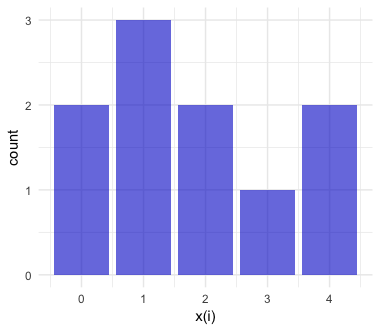
\includegraphics[width=\textwidth]{img/l01-problem2.png}
\end{center}
\end{minipage}
\begin{minipage}[c]{0.5\textwidth}
\begin{center}{\small
\begin{tabular}{cc}
\toprule
Patient ID ($i$) & $x^{(i)}$ \\
\midrule
1 & 4 \\
2 & 1 \\
3 & 0 \\
4 & 2 \\
5 & 2 \\
6 & 4 \\
7 & 3 \\
8 & 1 \\
9 & 0 \\
10 & 1 \\
\end{tabular}}
\end{center}
\end{minipage}
\vspace{3mm}

What distribution should you use to model these data? Calculate the MLE(s) for the parameter(s) of this distribution.
\vspace{3mm}

\item Same situation as above except that instead of taking a picture each day, the patient texts you at the moment he/she observes a rash. The data look like this, where $x^{(i)}$ is the time (in days) at which patient $i$ develops a rash: 

\begin{minipage}[c]{0.5\textwidth}
\begin{center}
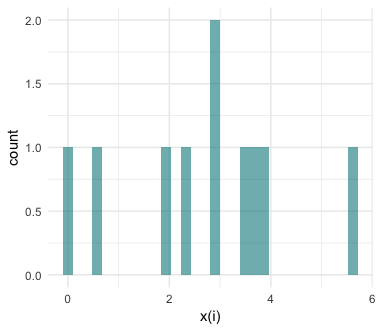
\includegraphics[width=\textwidth]{img/l01-problem3.png}
\end{center}
\end{minipage}
\begin{minipage}[c]{0.5\textwidth}
\begin{center}{\small
\begin{tabular}{cc}
\toprule
Patient ID ($i$) & $x^{(i)}$ \\
\midrule
1 & 2.25 \\
2 & 3.43\\
3 & 0.68\\
4 & 0.04\\
5 & 3.78\\
6 & 5.65\\
7 & 2.88\\
8 & 3.88\\
9 & 2.83\\
10 & 1.87\\
\end{tabular}}
\end{center}
\end{minipage}
\vspace{3mm}

What distribution should you use to model these data? Calculate the MLE(s) for the parameter(s) of this distribution.
\vspace{3mm}

\item Imagine you are Ladislaus Bortkiewicz, and you are modeling the number of persons killed by mule or horse kicks in the Prussian army per year. You have data from the late 1800s over the course of 20 years. Let $x^{(i)}$ be the number of deaths in year $i$.

\begin{minipage}[c]{0.5\textwidth}
\begin{center}
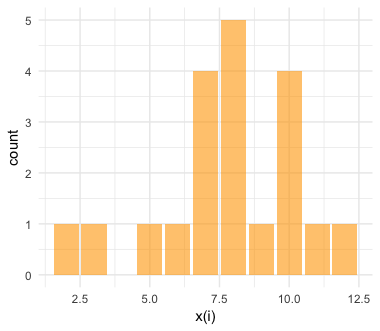
\includegraphics[width=\textwidth]{img/l01-problem4.png}
\end{center}
\end{minipage}
\begin{minipage}[c]{0.5\textwidth}
\begin{center}{\small
\begin{tabular}{cc|cc}
\toprule
Year ($i$) & $x^{(i)}$ & Year ($i$) & $x^{(i)}$ \\
\midrule
1 & 8 & 11 & 9 \\
2 & 10 & 12 & 7 \\
3 & 5 & 13 & 10 \\
4 & 3 & 14 & 12 \\
5 & 10 & 15 & 8 \\
6 & 8 & 16 & 7 \\
7 & 7 & 17 & 8 \\
8 & 2 & 18 & 8 \\
9 & 6 & 19 & 10 \\
10 & 11 & 20 & 7 \\
\end{tabular}}
\end{center}
\end{minipage}
\vspace{3mm}

What distribution should you use to model these data? Calculate the MLE(s) for the parameter(s) of this distribution.
\vspace{3mm}

\item You have waist circumference data on 1045 men aged 70 and above (see Dey's 2002 paper in the Journal of the American Geriatric Society). It looks like this:

\begin{center}
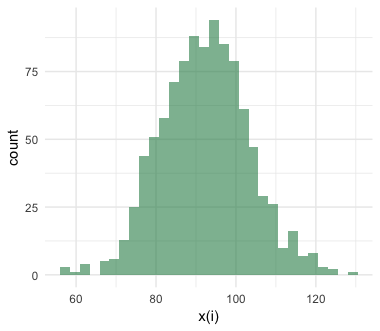
\includegraphics[width=0.5\textwidth]{img/l01-problem5.png}
\end{center}
\vspace{3mm}

What distribution should you use to model these data? Estimate the MLE(s) for the parameter(s) of this distribution.

\end{enumerate}

\chapter{Generalized Linear Models* \label{chapter:glms}}

Generalized linear models (GLMs) are a class of supervised learning models that form a convenient bridge between machine learning and traditional statistics. The basic idea behind a GLM is that your outcome variable (a.k.a. response variable, see Chapter~\ref{chapter:classification}), $y$, follows a probability distribution. The expected value, or mean, of that distribution is related to the values of the predictors (a.k.a. covariates; see Chapters~\ref{chapter:classification} and \ref{chapter:regression}), $x_1, \dots, x_p$ in a model-specific way.

We will focus on three classes of GLM: \textbf{linear regression}, which models data where the outcome, $y$, is numeric $\left( y \in \mathbb{R} \right)$; \textbf{logistic regression}, in which the outcome is binary $\left( y \in \{0, 1\} \right)$, and \textbf{loglinear (Poisson) regression}, in which the outcome is a positive integer, or count $\left( y \in \{0, 1, 2, \dots\} \right)$. We have seen linear regression already in Chapter~\ref{chapter:regression} and logistic regression in Chapter~\ref{chapter:classification}. There are many more GLMs corresponding to outcomes that follow other types of probability distributions. 

%%%%%%%%%%%%%%%%%%%%%%%%%%%%%%%%%%%%%%%%%%%%%%%%%%%%%%%%%%%%%%%%%%%%%%%%%%%%%%%

\section{Model Assumptions}

In GLMs, the predictors can be anything -- interval, ordinal, or nominal -- regardless of the specific model one chooses. However, there are several other assumptions that are important to consider before fitting one of these models:

\begin{itemize}
\item We assume that the outcome follows a certain type of distribution (e.g. Bernoulli distribution for a logistic regression model, normal for linear, etc.) conditional on the predictors. This assumption is baked into the model structure. It is, therefore, important to consider whether the outcome distribution you chose actually makes sense for your particular problem. It is generally not advisable to use a linear regression model, for example, when your outcome is a count. 
\item We assume that the predictors are fixed and known, and thus have no error associated with their measurements\footnote{Bayesian versions of these models relax this assumption, but we will not encounter these until much later}.
\item We assume that the predictors enter the model as a linear combination. This is why GLMs are referred to as ``linear models''. 
\item We assume that the $n$ samples in our dataset are collected independently, so that the errors of the $n$ sample outcomes are uncorrelated\footnote{Think back to our formulation of the likelihood in Chapter~\ref{chapter:mlebasics} and how it depended on the samples' being independent and identically distributed, or iid.}.
\end{itemize}

%%%%%%%%%%%%%%%%%%%%%%%%%%%%%%%%%%%%%%%%%%%%%%%%%%%%%%%%%%%%%%%%%%%%%%%%%%%%%%%

\section{Modeling the Predictors}

All of the GLMs we will see today incorporate a \textbf{linear combination} of predictors. A linear combination is an expression constructed from a set of terms by multiplying each term by a constant and adding the results. We denote the number of predictors in the model by $p$ and the vector of predictors by $x$, where
$$ x = \begin{bmatrix}
1 \\
           x_{1} \\
           x_{2} \\
           \vdots \\
           x_{p}
         \end{bmatrix} $$
and we have included a ``1'' as the first element to allow for an \textbf{intercept}. We write $x^{(i)}$ to denote the vector of predictors associated with the $i$th training example. The coefficients of the linear combination (i.e. the model parameters we are hoping to learn) are denoted by:
$$ \beta = \begin{bmatrix}
\beta_0 \\
           \beta_{1} \\
           \beta_{2} \\
           \vdots \\
           \beta_{p}
         \end{bmatrix} $$
and we often express the linear combination as an inner product, written as
$$ \beta^T x = \beta_0 + \sum_{j=1}^p \beta_j x_j. $$

Generalized linear models model the \textbf{expected value} of the outcome, $E[y]$, as a function of this linear combination of predictors. The function that relates the two is called the \textbf{link function}. Different types of GLM use different link functions.

%%%%%%%%%%%%%%%%%%%%%%%%%%%%%%%%%%%%%%%%%%%%%%%%%%%%%%%%%%%%%%%%%%%%%%%%%%%%%%%

\section{Linear Regression}

The linear regression model has a long history of development before the advent of GLMs, so it's typically taught in its own course with all of the associated model diagnostics, goodness of fit tests, etc. long before a student ever sees other GLMs. I think a comparative approach is more effective, which is why we're doing it this way\footnote{The other thing about linear regression models is that they are usually fit using least squares methods instead of maximum likelihood. The parameter estimates are the same in both cases, as we will see much later.}.

\subsection{Modeling the Outcome} 

In linear regression, we assume that the outcome, $y$, follows a normal distribution (see Section~\ref{sect:normal}), conditional on the values of the predictors. Recall that the normal distribution is a continuous probability distribution with the following properties:
$$ p(y | \mu, \sigma) = \frac{1}{\sqrt{2 \pi \sigma^2}} e^{-\frac{(y-\mu)^2}{2 \sigma^2}} \qquad  E[y| \mu, \sigma] = \mu \qquad \text{var}(y | \mu, \sigma) = \sigma^2 $$
where $y \in \mathbb{R}$.

\subsection{Linking the Predictors to the Outcome}

In linear regression, the mean of the outcome distribution, which is normal, can be any real number. We therefore use the \textbf{identity link}, setting $E[y]$ directly equal to the linear combination of predictors. Since the outcome is normal, we know that $E[y] = \mu$, the mean of the normal distribution. We therefore write:
\begin{equation} E[y] = \mu = \beta^T x \label{eqn:meanlinear} \end{equation}
which is usually rearranged and rewritten as:
$$ y = \beta^T x + \varepsilon $$
where $\varepsilon \sim N(0, \sigma^2)$. The relationship between $E[y]$ and $\beta^T x$ is shown below.

\begin{center}
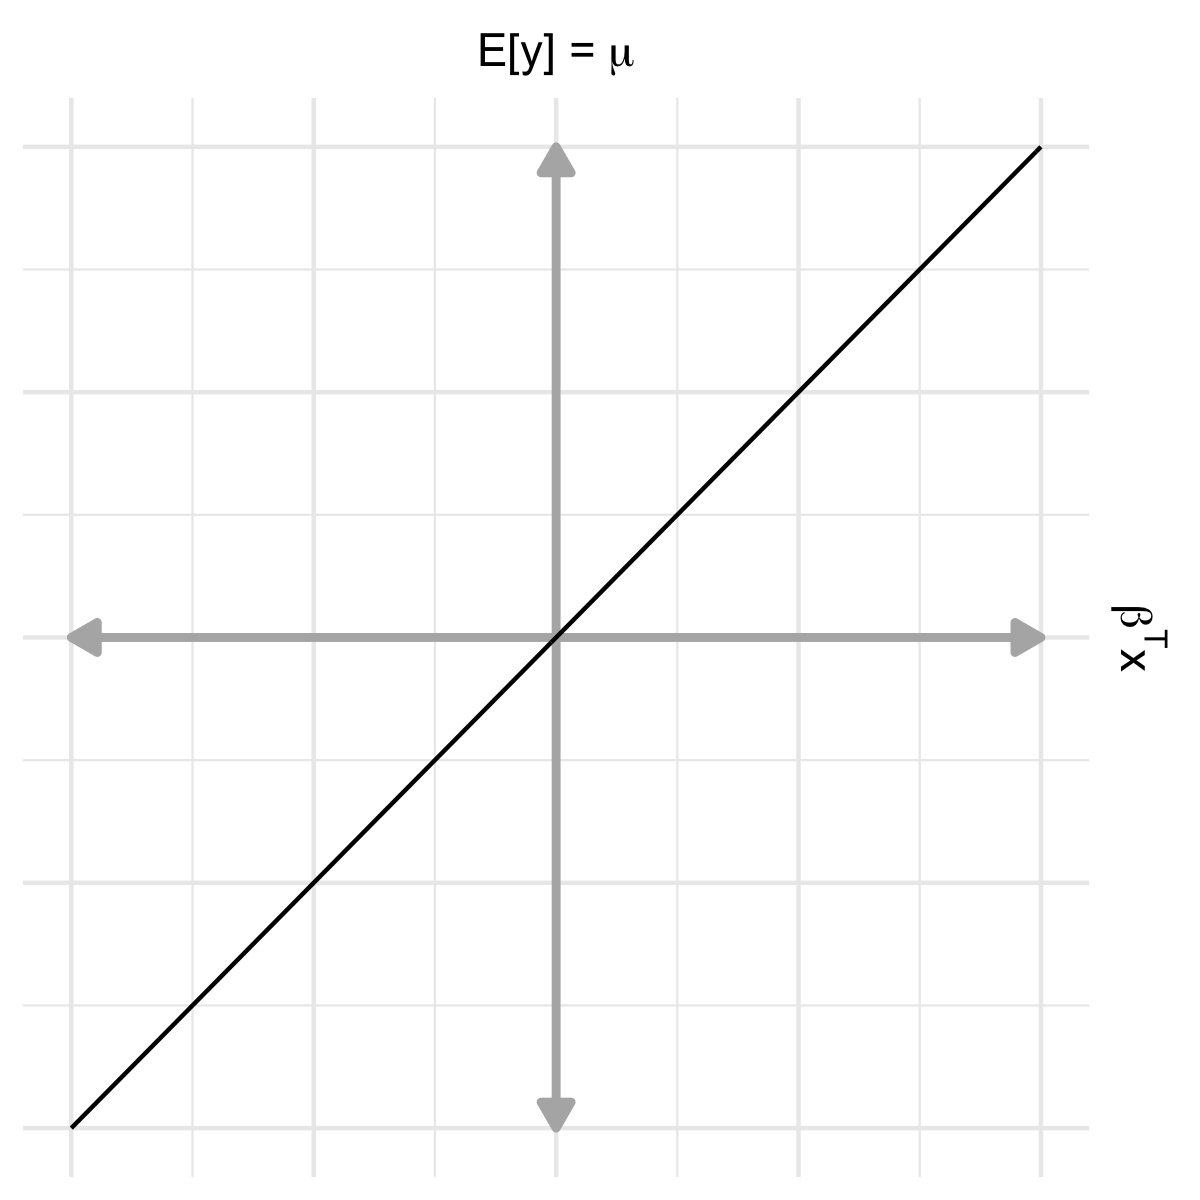
\includegraphics[width=0.5\textwidth]{img/l02-figure1-linreg.png}
\end{center}

%%%%%%%%%%%%%%%%%%%%%%%%%%%%%%%%%%%%%%%%%%%%%%%%%%%%%%%%%%%%%%%%%%%%%%%%%%%%%%%

\section{Logistic Regression}

Logistic regression models data where the outcome is binary; i.e. where $y$ is ``yes'' or ``no''. Variants of logistic regression, called \textbf{multinomial logistic regression} and the \textbf{proportional odds model}, can also be used to model data where the outcome contains multiple categories that either have an ordering (ordinal) or do not (nominal). We will see how this works in a second.

\subsection{Modeling the Outcome}

In logistic regression the outcome, $y$, is either $0$ or $1$. We model it using the Bernoulli distribution (see Section~\ref{sect:bernoulli}), which is a discrete probability distribution with the following properties:
$$ p(y|\mu) = \mu^y (1 - \mu) ^ {1-y} \qquad E[y| \mu] = \mu \qquad \text{var}(y | \mu) = \mu (1 - \mu) $$
where $y \in \{0, 1\}$.

\subsection{Linking the Predictors to the Outcome}

In logistic regression, the mean of the outcome distribution, which is Bernoulli, is a probability. It must therefore be a real number between 0 and 1. No matter how large or small $\beta^T x$ gets, the value of $E[y] = \mu$ cannot be outside this range. We therefore apply the \textbf{logistic function}, $f(x) = 1/(1 + \exp(-x))$, which has the range $(0, 1)$, to $\beta^T x$ to squash it:
\begin{equation} E[y] = \mu = \frac{1}{1 + \exp{(-\beta^Tx)}} \label{eqn:meanlogistic} \end{equation}
The relationship between $E[y]$ and $\beta^T x$ is shown below. We typically invert the model to write
$$ \log{\frac{\mu}{1-\mu}} = \beta^T x $$
which is the standard form of the logistic regression model. The function $\log \left( \mu/(1-\mu) \right)$ is called the logit, and in logistic regression we say we use the \textbf{logit link}.

\begin{center}
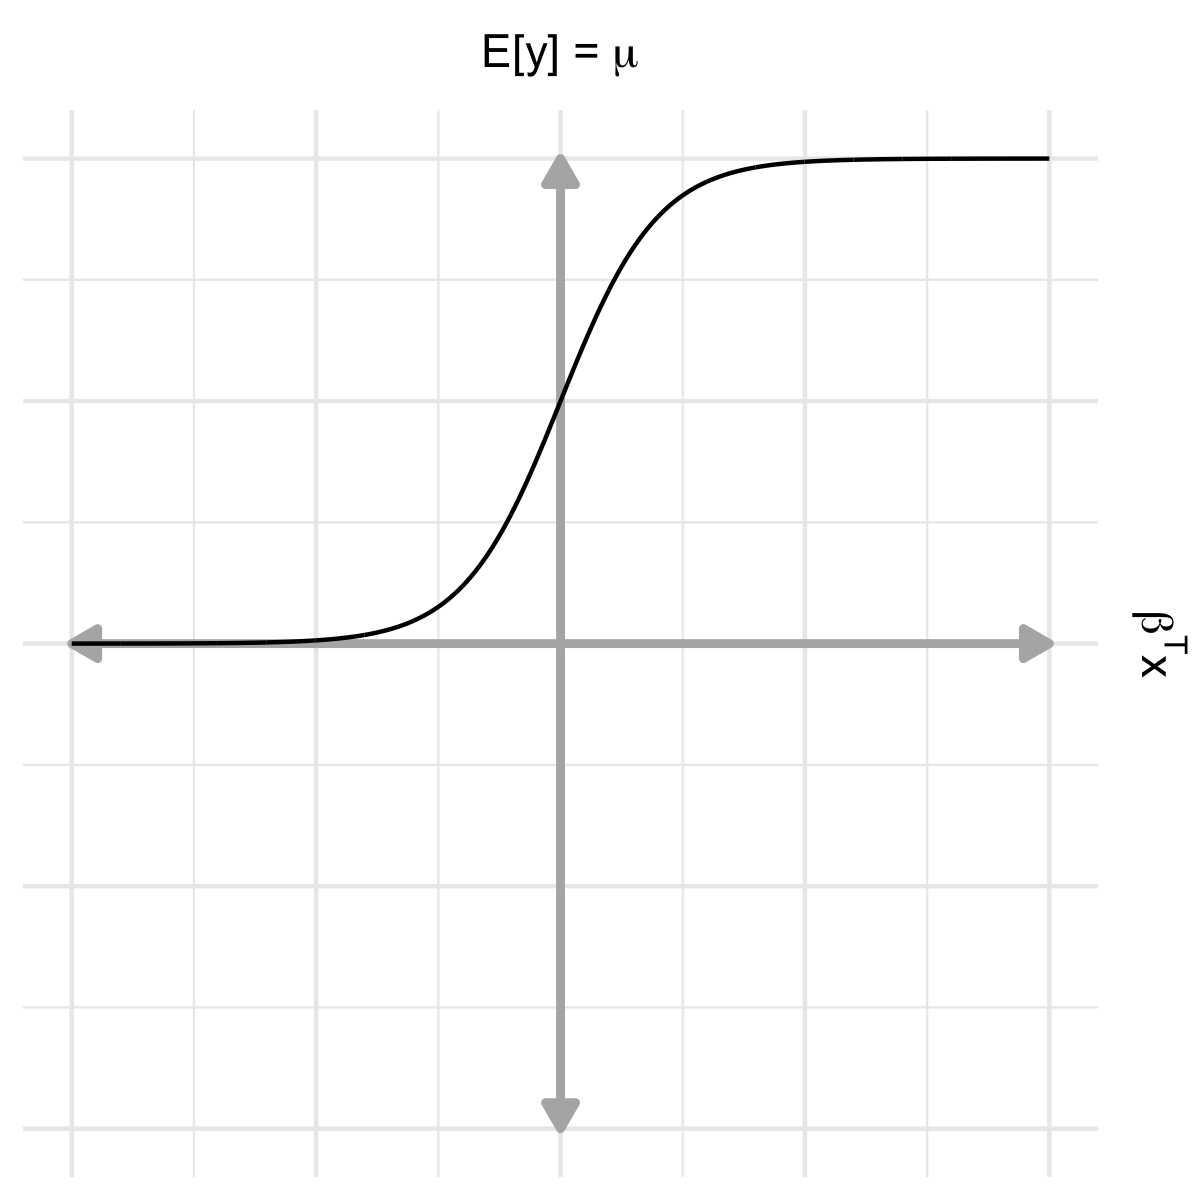
\includegraphics[width=0.5\textwidth]{img/l02-figure2-logistic.png}
\end{center}

%%%%%%%%%%%%%%%%%%%%%%%%%%%%%%%%%%%%%%%%%%%%%%%%%%%%%%%%%%%%%%%%%%%%%%%%%%%%%%%

\section{Poisson Regression}

In Poisson regression, the outcome is a count. This type of regression is less common than linear and logistic regression, but we include it here mainly so you can see how the ideas from GLM extend to many different classes of outcome distributions within the exponential family.  

\subsection{Modeling the Outcome}

In Poisson regression, we model the outcome using the Poisson distribution, which is a discrete probability distribution with the following properties:
$$ p(y | \lambda) = \frac{e^{-\lambda} \lambda^y}{y!} \qquad E[y|\lambda] = \lambda \qquad \text{var}(y|\lambda) = \lambda $$
where $y \in 0, 1, 2, \dots$.

\subsection{Linking the Predictors to the Outcome}

In Poisson regression, the mean of the outcome distribution, which is Poisson, is the expected value of a count. It must therefore be a real number greater than or equal to zero. In particular, no matter how small $\beta^T x$ gets, the value of $E[y] = \lambda$ cannot be negative. We therefore exponentiate $\beta^T x$ to ensure that the result is greater than zero:
\begin{equation} E[y] = \lambda = \exp(\beta^T x) \label{eqn:meanpoisson} \end{equation}
The relationship between $E[y]$ and $\beta^T x$ is shown below. We typically invert the model to write
$$ \log(\lambda) = \beta^T x $$
which is the standard form of the Poisson regression model. We say we use the \textbf{log link}. 

\begin{center}
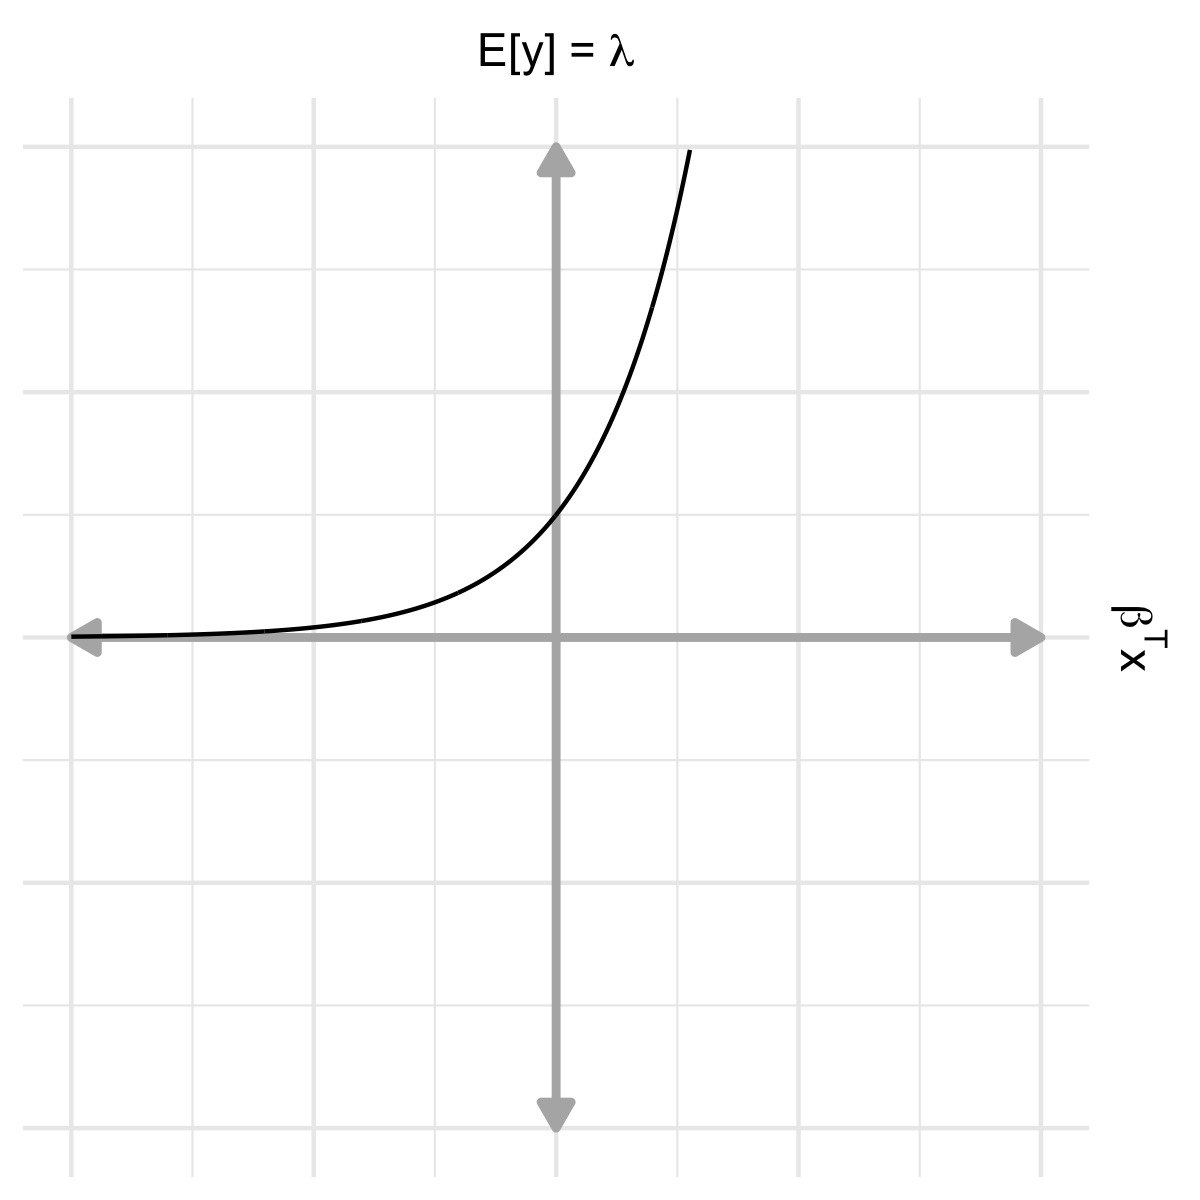
\includegraphics[width=0.5\textwidth]{img/l02-figure3-poisson.png}
\end{center}

%%%%%%%%%%%%%%%%%%%%%%%%%%%%%%%%%%%%%%%%%%%%%%%%%%%%%%%%%%%%%%%%%%%%%%%%%%%%%%%

\section{Maximum Likelihood for GLMs}

GLMs are typically fit using maximum likelihood estimation (see Chapter~\ref{chapter:mlebasics}). A full treatment of MLE for GLMs is outside the scope of these notes, but I've put the start of the calculations for each type of model below.    

\subsection{Linear Regression} 

The likelihood for the linear regression model is:
$$ \mathcal{L}(\mu^{(1)}, \dots, \mu^{(n)}, \sigma) = \prod_{i=1}^n \frac{1}{\sqrt{2 \pi \sigma^2}} \exp \left[ - \frac{(y^{(i)} - \mu^{(i)})^2}{2 \sigma^2} \right] $$
where we use $\mu^{(i)}$ to represent the model's estimate of the mean of the outcome at the position of training example $i$. We can use Equation~\ref{eqn:meanlinear} to rewrite this as a function of the predictors:
$$ \mathcal{L}(\beta, \sigma) = \prod_{i=1}^n \frac{1}{\sqrt{2 \pi \sigma^2}} \exp \left[ - \frac{(y^{(i)} - \beta^T x^{(i)})^2}{2 \sigma^2} \right] $$
Taking the log, we obtain the log-likelihood:
$$ \log \mathcal{L}(\beta, \sigma) = -\frac{n}{2} \log (2 \pi) - \frac{n}{2} \log(\sigma^2) - \frac{1}{2 \sigma^2} \sum_{i=1}^n \left( y^{(i)} - \beta^T x^{(i)} \right)^2 $$
Taking derivatives of the log-likelihood with respect to the $\beta$s, we find that we can maximize the likelihood by minimizing the sum-squares: $\sum_{i=1}^n \left( y^{(i)} - \beta^T x^{(i)} \right)^2$.

\subsection{Logistic Regression}

The likelihood for the logistic regression model is:
$$ \mathcal{L}(\mu^{(1)}, \dots, \mu^{(n)}) = \prod_{i=1}^n {\mu^{(i)}}^{y^{(i)}} (1-\mu^{(i)})^{1 - y^{(i)}} $$
Rewriting this as a function of the predictors, we get:
$$ \mathcal{L}(\beta) = \prod_{i=1}^n \left( \frac{1}{1 + \exp(-\beta^T x^{(i)})} \right)^{y^{(i)}} \left( \frac{\exp(-\beta^T x^{(i)})}{1 + \exp(-\beta^T x^{(i)})} \right)^{1 - y^{(i)}} $$
Taking the log, we obtain the log-likelihood:
$$ \log \mathcal{L}(\beta) = \sum_{i=1}^n \left[ -y^{(i)} \log \left[ 1 + \exp(-\beta^T x^{(i)}) \right] + (1 -y^{(i)}) \log \left[ 1 + \exp(-\beta^T x^{(i)}) \right] \right] $$
Again, we will take derivatives of the log-likelihood with respect to the $\beta$s to maximize it. However, we cannot solve for the optimal $\beta$s analytically; numerical optimization methods are used to perform the optimization.

\subsection{Loglinear (Poisson) Regression}

The likelihood for the Poisson regression model is:
$$ \mathcal{L}(\lambda^{(1)}, \dots, \lambda^{(n)}) = \prod_{i=1}^n \frac{{\lambda^{(i)}}^{y^{(i)}} e^{-\lambda^{(i)}}}{y^{(i)}!} $$
Rewriting this as a function of the predictors, we get:
$$ \mathcal{L}(\beta) = \prod_{i=1}^n \frac{\exp{(y^{(i)} \beta^T x^{(i)})} e^{-\exp{(\beta^T x^{(i)})}}}{y^{(i)}!} $$
Taking the log, we obtain the log-likelihood:
$$ \log \mathcal{L}(\beta) = \sum_{i=1}^n \left[ y^{(i)} \beta^T x^{(i)} - \exp(\beta^T x^{(i)}) - \log (y^{(i)}!) \right] $$
As with logistic regression, we cannot solve for the optimal $\beta$s analytically; numerical optimization methods are used. 

\chapter{Fitting and Interpreting GLMs \label{chapter:fitglm}}

Generalized linear models (Chapter~\ref{chapter:glms}) are just one way to approach supervised learning. However, they are by far the most common approach in the clinical research literature. Linear and logistic regression are established, standard methods for clinical data analysis in contexts where you want to relate the effects of one or more predictors to an outcome that is a number or a class (e.g. yes/no). Because of this, it is important to know how to interpret these models -- e.g., what the coefficients, standard errors, and model diagnostics mean -- and how to fit them using software. 

%%%%%%%%%%%%%%%%%%%%%%%%%%%%%%%%%%%%%%%%%%%%%%%%%%%%%%%%%%%%%%%%%%%%%%%%%%%%%%%

\section{Examples from Chapters~\ref{chapter:classification} and \ref{chapter:regression} \label{sect:clregexamples}}

In Chapter~\ref{chapter:classification}, we saw an example where information about two predictors -- a disease severity score ($x_1$) and a social determinants score ($x_2$) -- was used to predict a binary outcome: whether a patient would be readmitted to the ER within 30 days of discharge. In Chapter~\ref{chapter:regression}, we used the same two predictors to predict the numeric level of a disease recurrence biomarker. Here are pictures of the logistic regression model from Chapter~\ref{chapter:classification} and the linear regression model from Chapter~\ref{chapter:regression} with their fitted model summary output. Note: These pictures include axis labels, whereas those from Chapters~\ref{chapter:classification} and \ref{chapter:regression} did not. 

\begin{center}
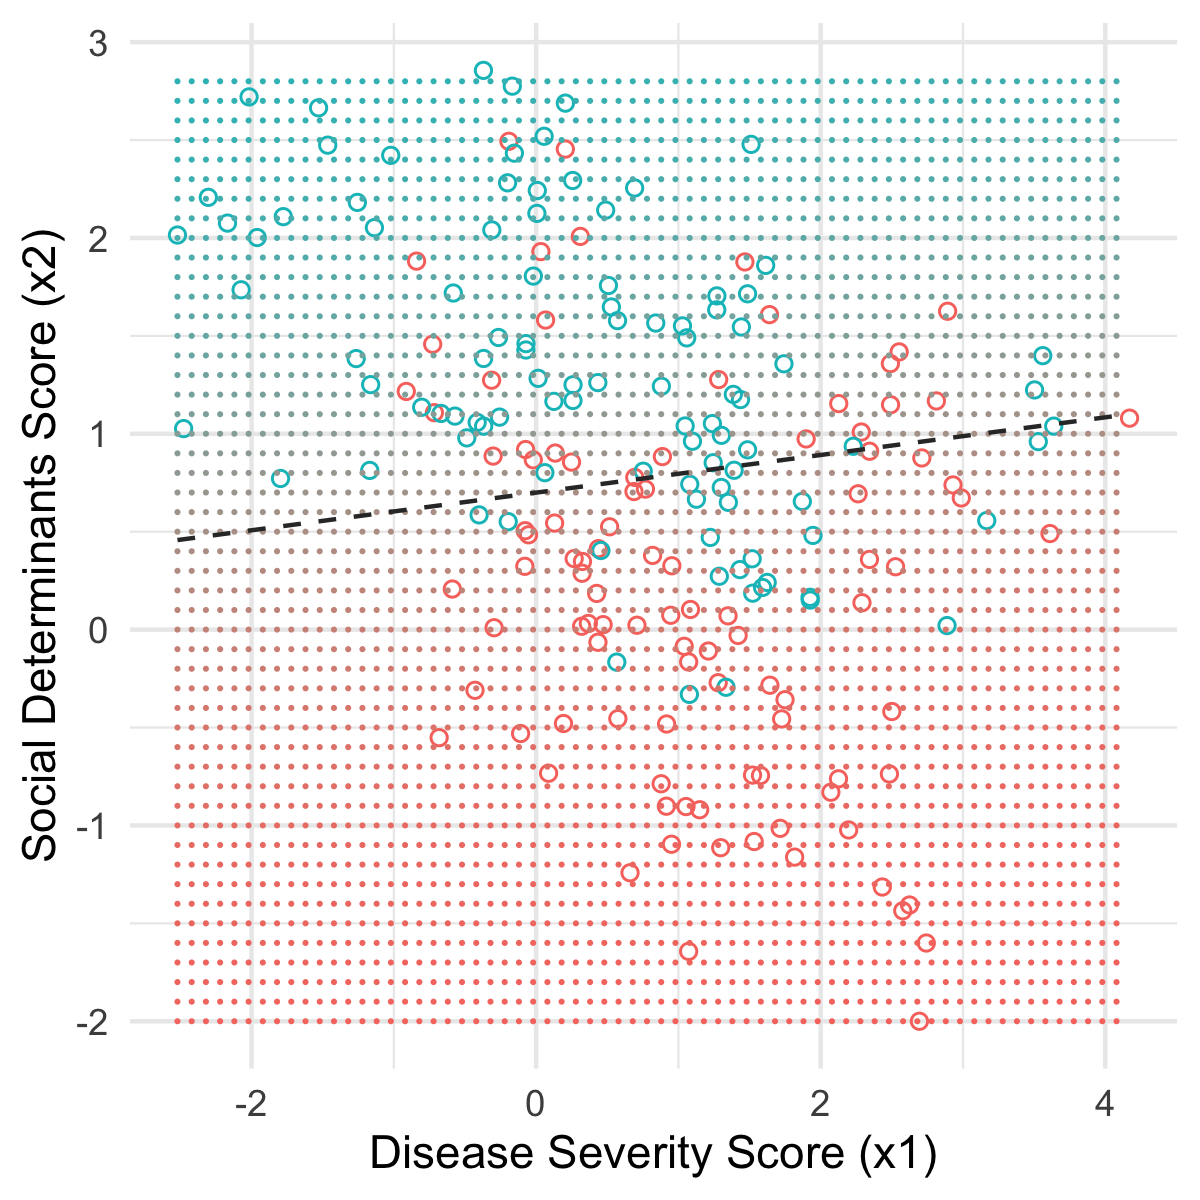
\includegraphics[width=0.35\textwidth]{img/esl-logistic-prob-axes.png}
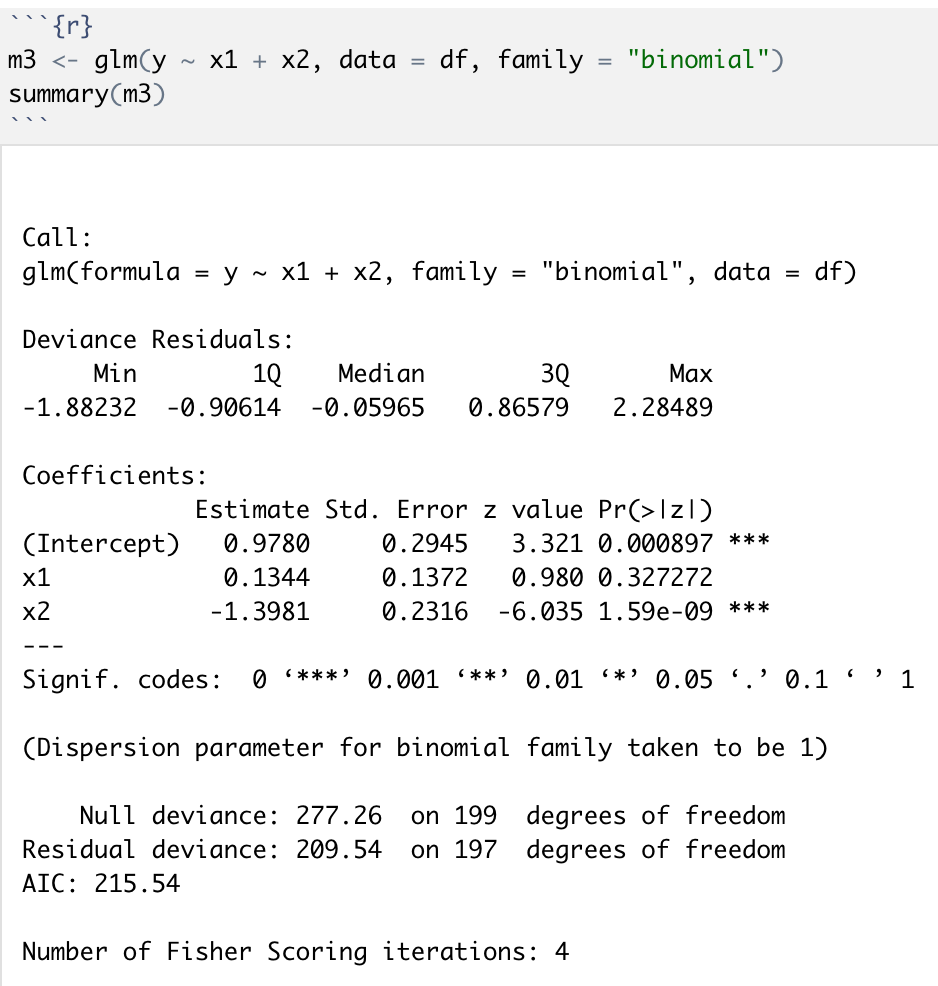
\includegraphics[width=0.64\textwidth]{img/glm-binomial-example.png}\\[8mm]
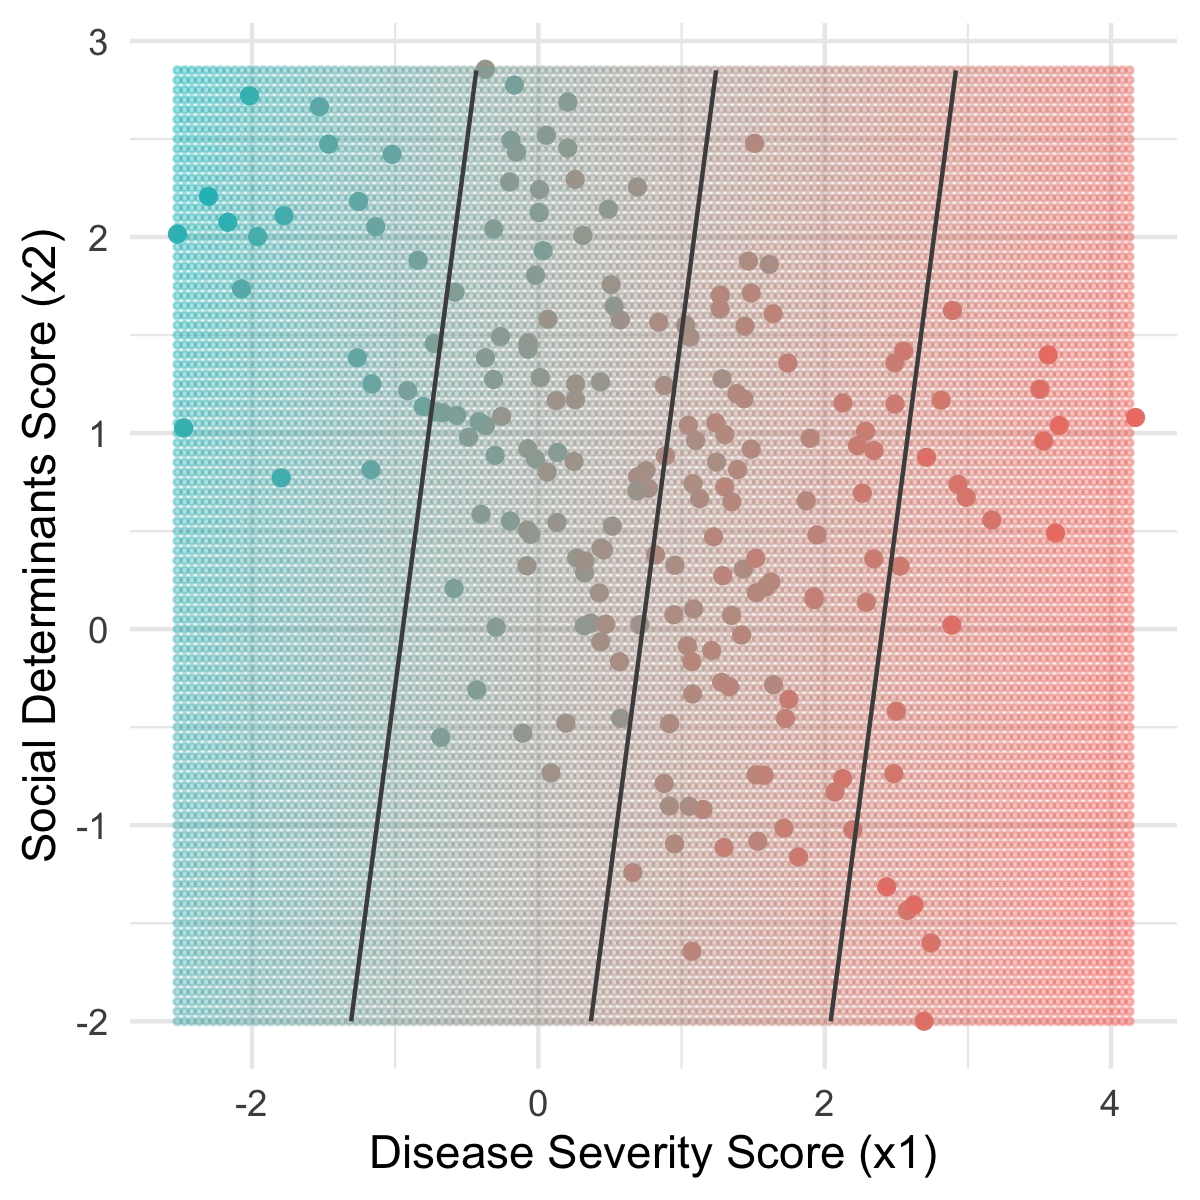
\includegraphics[width=0.35\textwidth]{img/esl-reg-linear-wlabels.png}
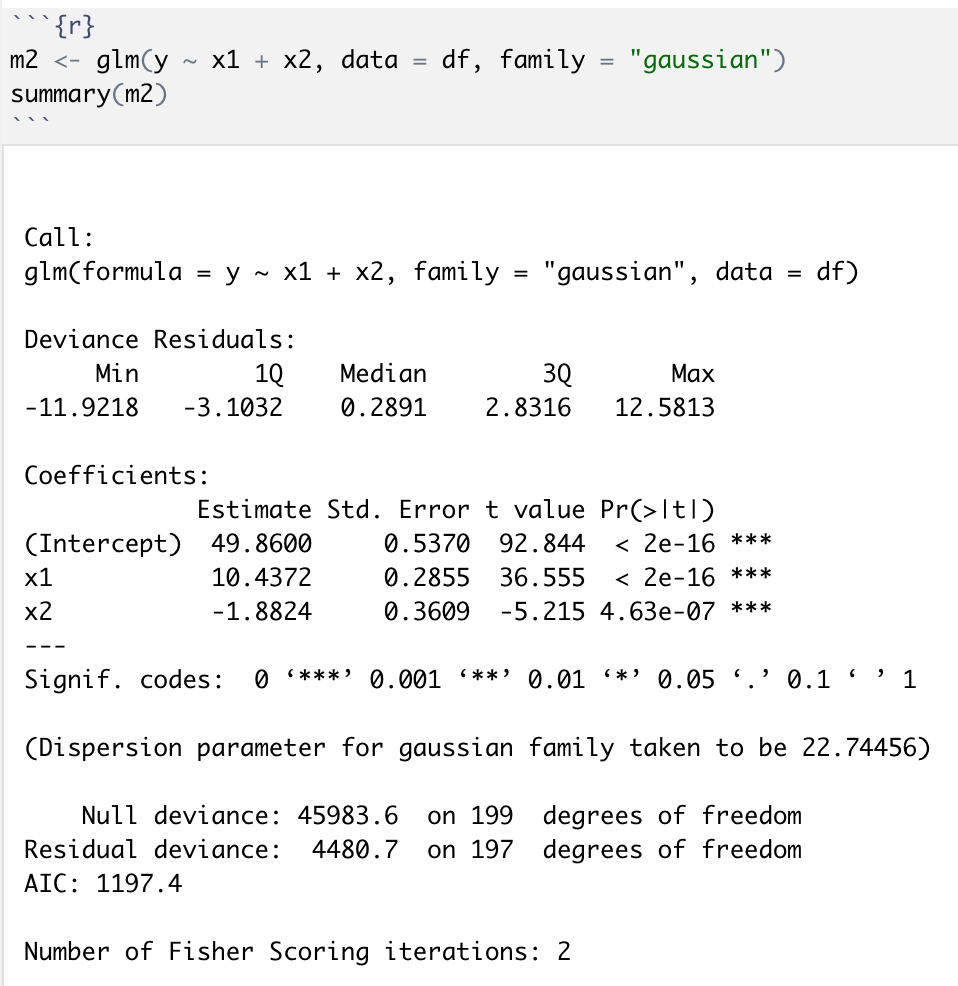
\includegraphics[width=0.64\textwidth]{img/glm-gaussian-example.png}
\end{center}

\begin{question}{}
Interpret the meaning of the coefficients of $x_1$ and $x_2$ in the linear regression model.
\end{question}

\begin{question}{}
Interpret the meaning of the intercept in the linear regression model.
\end{question}

\begin{question}{}
Interpret the meaning of the coefficients of $x_1$ and $x_2$ in the logistic regression model.
\end{question}

\begin{question}{}
Interpret the meaning of the intercept in the logistic regression model.
\end{question}

%%%%%%%%%%%%%%%%%%%%%%%%%%%%%%%%%%%%%%%%%%%%%%%%%%%%%%%%%%%%%%%%%%%%%%%%%%%%%%%

\section{Standard Errors and Hypothesis Tests}

The magnitudes of the coefficients in these models matter only in relation to:
\begin{enumerate}
\item The scale on which the predictors are measured. 
\item The amount of uncertainty the model has about their values.
\end{enumerate}
For example, if a predictor varies only across a tiny range of values, its model coefficient may be large, since it quantifies the change in the link-function-transformed outcome when the predictor changes by 1.0. However, that doesn't mean that the predictor itself is important to the outcome\footnote{This is one reason many advocate \textbf{scaling} and \textbf{centering} predictors before fitting a model. Centering means subtracting the mean value of a predictor from all of its individual measurements so that the mean of each centered predictor is zero. Scaling means dividing the values of each predictor by their standard deviation, so that the standard deviation of each predictor is 1.0. This enables the relative magnitudes of the model coefficients to be compared directly.}.

Similarly, the model may be highly uncertain about a coefficient's value, owing to factors like a small dataset (small $n$) or collinearity among the predictors. Mathematically, high uncertainty means that the value of the likelihood doesn't change very rapidly as you move away from the maximum likelihood estimate of a coefficient. For example, here is how the log-likelihood for the logistic regression example above changes when we vary $\beta_1$ (the coefficient of $x_1$), keeping $\beta_0$ (the intercept) and $\beta_2$ (the coefficient of $x_2$) fixed at their MLEs: 
\begin{center}
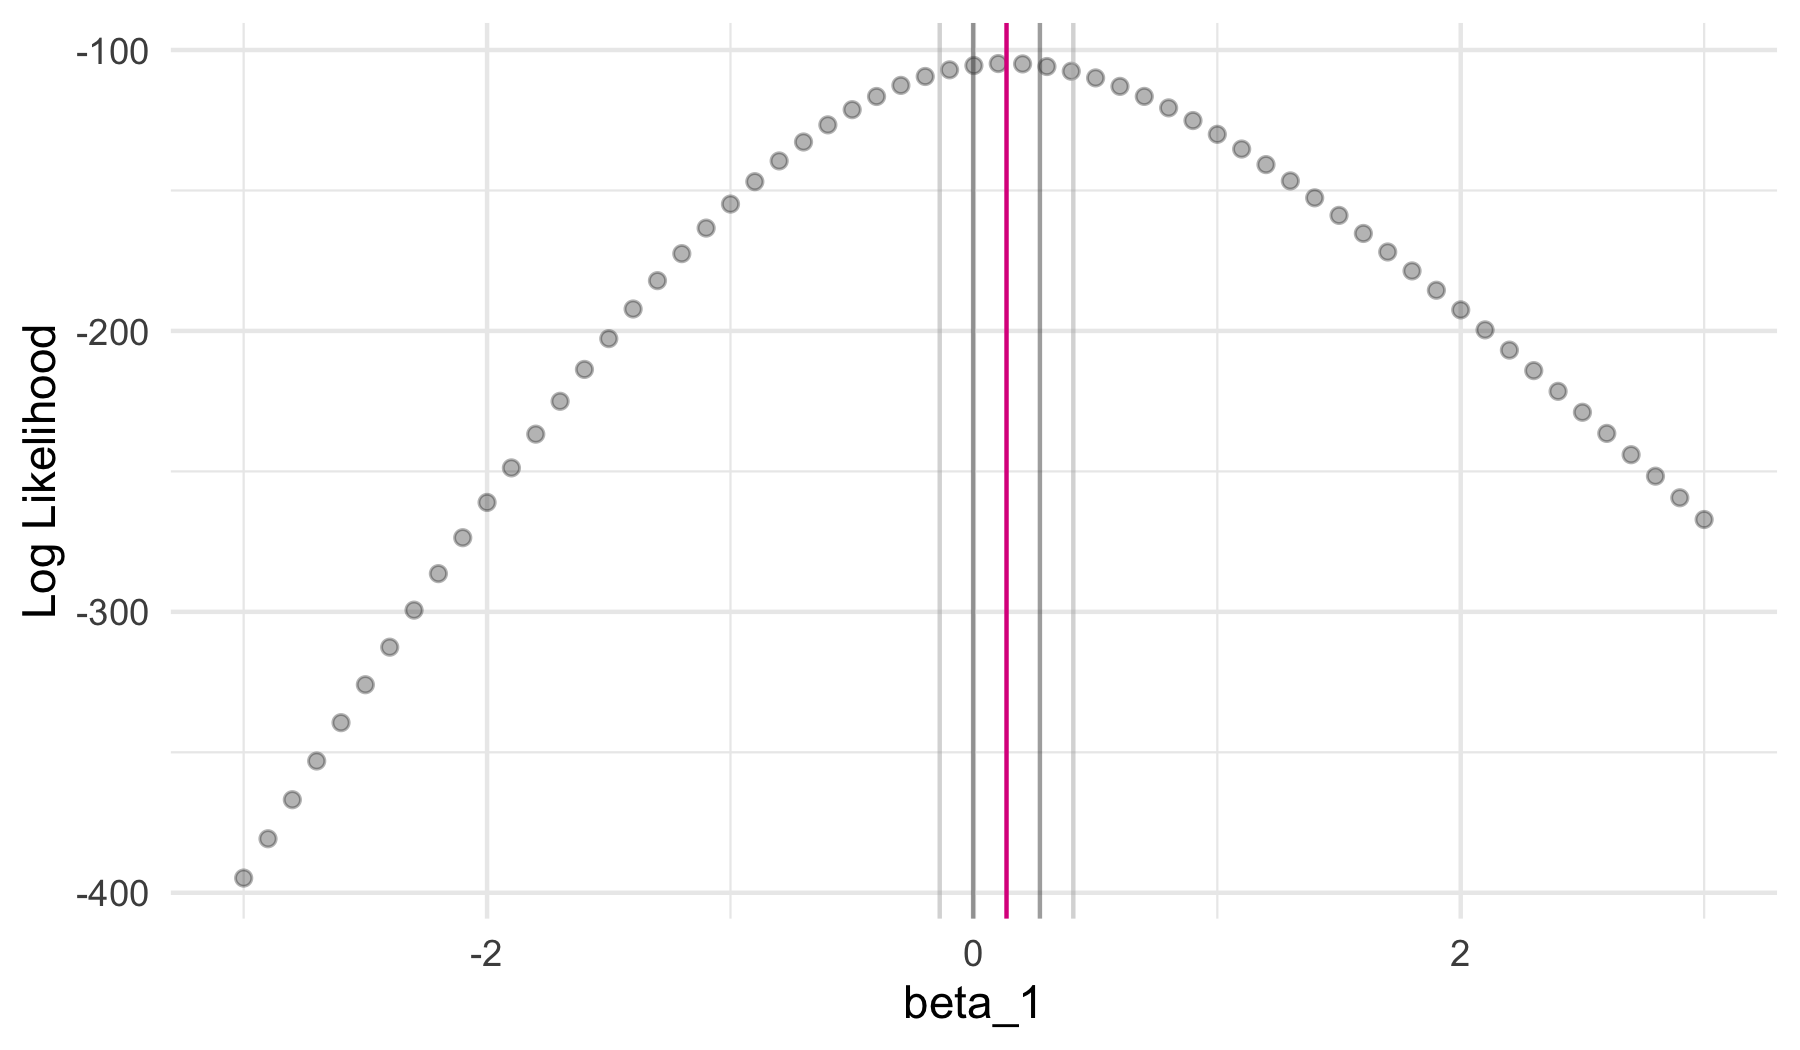
\includegraphics[width=0.7\textwidth]{img/esl-logistic-beta1.png}
\end{center}
The gray vertical lines are related to the \textbf{standard error} of the model coefficient, which is in turn related to the ``flatness'' of the likelihood surface around the MLE. The gray lines are situated at 1 and 2 standard errors away from the MLE in either direction. You can see that in the case of $\beta_1$, the gray lines overlap zero. The value zero (no effect) is a plausible estimate of the impact of $x_1$ on the outcome. 

Contrast this with how the log-likelihood varies around the MLE for $\beta_2$:
\begin{center}
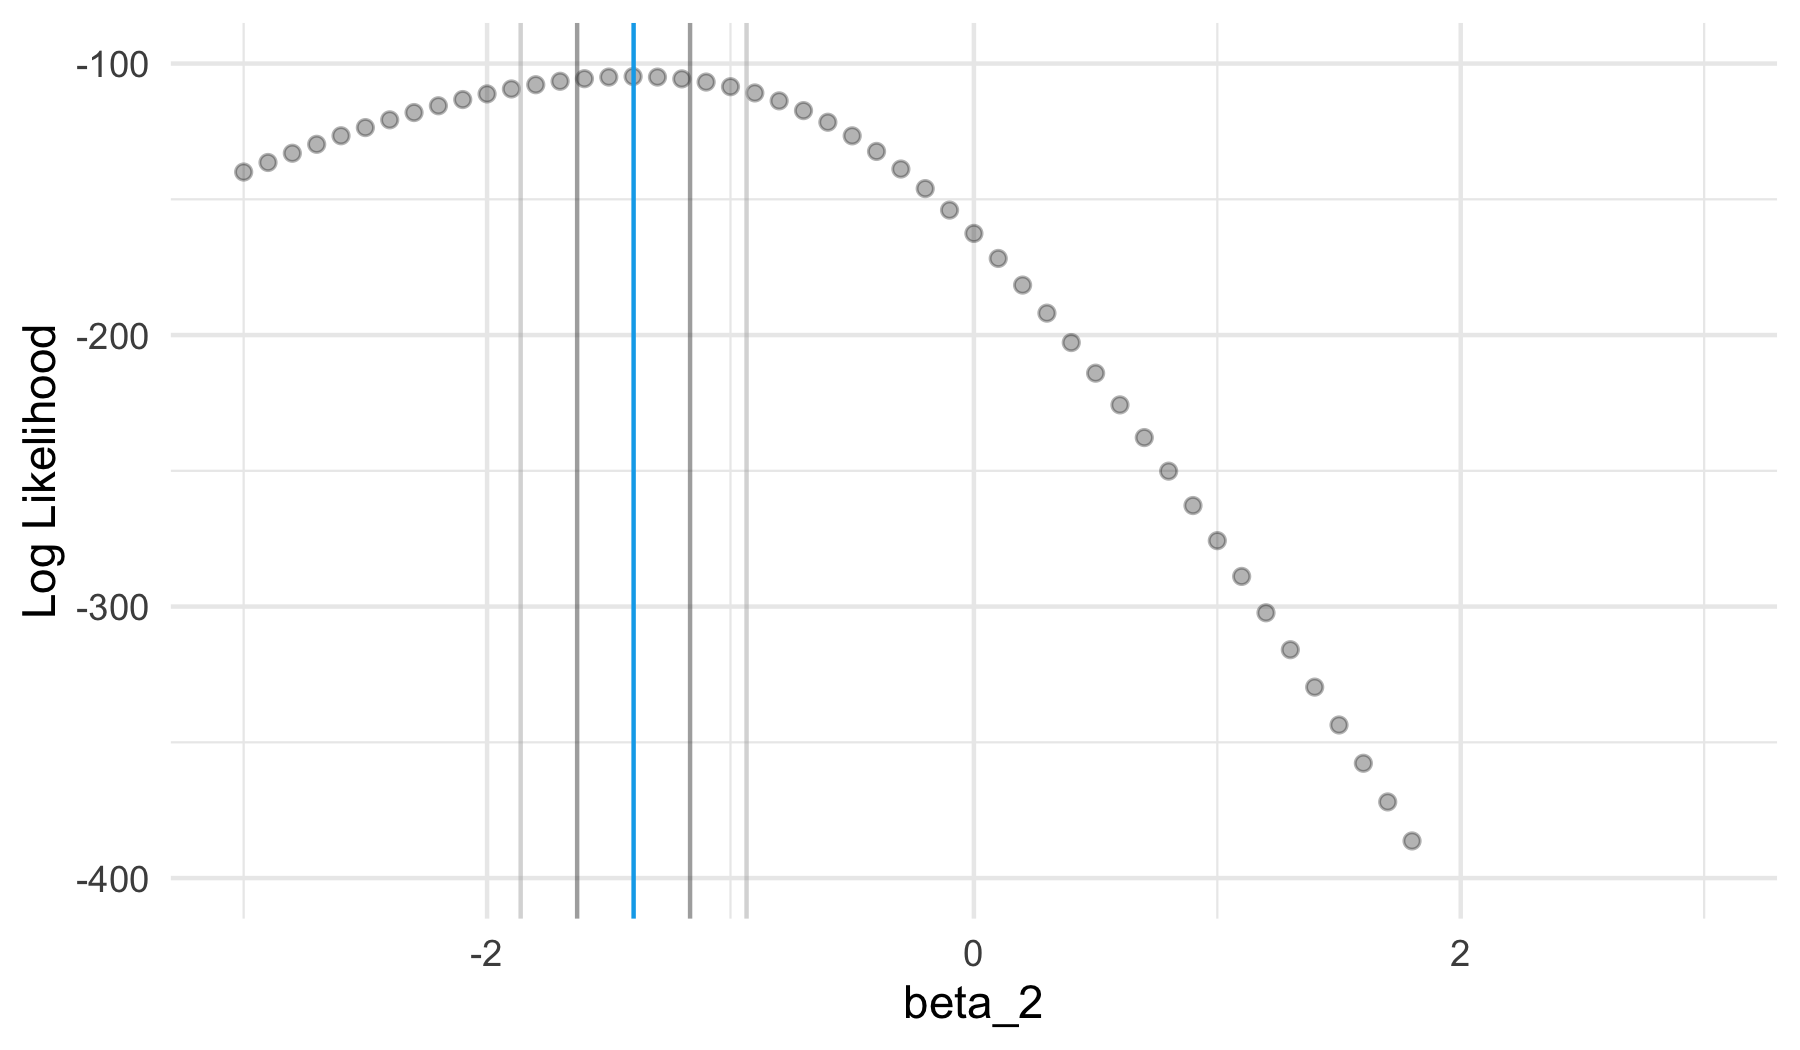
\includegraphics[width=0.7\textwidth]{img/esl-logistic-beta2.png}
\end{center}
Here the standard error is larger, but the magnitude of the coefficient is also larger, so the range of the gray lines does not overlap zero. These findings are reflected in the relative values of the \textbf{Z-statistic} (\texttt{z value}) and \textbf{P-value} (\verb|Pr(>|z|)|) in the model output for the two coefficients. Whether a coefficient's value is likely to be nonzero is typically evaluated using a formalism called a \textbf{hypothesis test}. We will discuss hypothesis tests in much greater detail in Chapter~\ref{chapter:hypothesistesting}.  

%%%%%%%%%%%%%%%%%%%%%%%%%%%%%%%%%%%%%%%%%%%%%%%%%%%%%%%%%%%%%%%%%%%%%%%%%%%%%%%

\section{Case Study: Linear Regression}

The following data come from an early study that examined the possible link between air pollution and mortality. The authors examined 60 cities throughout the United States and recorded the following data:
\begin{center}
\texttt{ \small \begin{tabular}{ll}
\toprule
MORT & Total age-adjusted mortality from all causes, \\
& in deaths per 100,000 population \\
PRECIP & Mean annual precipitation (in inches) \\
EDUC & Median number of school years completed \\
& for persons of age 25 years or older \\
NONWHITE & Percentage of the 1960 population that is nonwhite \\
NOX & Relative pollution potential of oxides of nitrogen \\
SO2 & Relative pollution potential of sulfur dioxide \\
\bottomrule
\end{tabular}
}
\end{center}
Note: ``Relative pollution potential'' refers to the product of the tons emitted per day per square kilometer and a factor correcting the SMSA dimensions and exposure.

We want to predict the value of \texttt{MORT} ($y$) using the predictors \texttt{PRECIP, EDUC, NONWHITE, NOX,} and \verb|SO2| ($x_1, x_2, x_3, x_4$ and $x_5$). Here is the GLM output for this model in R:
{\small
\begin{verbatim}
Call:
glm(formula = MORT ~ PRECIP + EDUC + NONWHITE + NOX + SO2, 
    family = "gaussian", data = d)

Deviance Residuals: 
   Min      1Q  Median      3Q     Max  
-91.38  -18.97   -3.56   16.00   91.83  

Coefficients:
             Estimate Std. Error t value Pr(>|t|)    
(Intercept) 995.63646   91.64099  10.865 3.35e-15 ***
PRECIP        1.40734    0.68914   2.042 0.046032 *  
EDUC        -14.80139    7.02747  -2.106 0.039849 *  
NONWHITE      3.19909    0.62231   5.141 3.89e-06 ***
NOX          -0.10797    0.13502  -0.800 0.427426    
SO2           0.35518    0.09096   3.905 0.000264 ***
---
Signif. codes:  0 '***' 0.001 '**' 0.01 '*' 0.05 '.' 0.1 ' ' 1

(Dispersion parameter for gaussian family taken to be 1375.723)

    Null deviance: 228275  on 59  degrees of freedom
Residual deviance:  74289  on 54  degrees of freedom
AIC: 611.56

Number of Fisher Scoring iterations: 2
\end{verbatim}
}

Side note: Most models can be fit multiple ways. Linear regression models are normally fit using \textbf{ordinary least squares} and the \verb|lm| package, as opposed to maximum likelihood and the \verb|glm| package. The coefficients and most of the output are exactly the same:

{\small
\begin{verbatim}
Call:
lm(formula = MORT ~ PRECIP + EDUC + NONWHITE + NOX + SO2, 
   data = d)

Residuals:
   Min     1Q Median     3Q    Max 
-91.38 -18.97  -3.56  16.00  91.83 

Coefficients:
             Estimate Std. Error t value Pr(>|t|)    
(Intercept) 995.63646   91.64099  10.865 3.35e-15 ***
PRECIP        1.40734    0.68914   2.042 0.046032 *  
EDUC        -14.80139    7.02747  -2.106 0.039849 *  
NONWHITE      3.19909    0.62231   5.141 3.89e-06 ***
NOX          -0.10797    0.13502  -0.800 0.427426    
SO2           0.35518    0.09096   3.905 0.000264 ***
---
Signif. codes:  0 '***' 0.001 '**' 0.01 '*' 0.05 '.' 0.1 ' ' 1

Residual standard error: 37.09 on 54 degrees of freedom
Multiple R-squared:  0.6746,  Adjusted R-squared:  0.6444 
F-statistic: 22.39 on 5 and 54 DF,  p-value: 4.407e-12
\end{verbatim}
}

\begin{question}{}
Interpret the values of each of these coefficients. Based on the coefficient values and their standard errors, which predictor(s) do you think have the greatest impact on mortality? 
\end{question}

\begin{question}{}
In this model, is the effect of one predictor (say, \verb|PRECIP|) impacted by the value(s) of any of the other predictor(s)? How does this differ from the other regression algorithms we've seen (KNN and decision trees)? What are the advantages and disadvantages of this choice? 
\end{question}

%%%%%%%%%%%%%%%%%%%%%%%%%%%%%%%%%%%%%%%%%%%%%%%%%%%%%%%%%%%%%%%%%%%%%%%%%%%%%%%

\section{Case Study: Logistic Regression}

The goal of this study was to identify risk factors associated with giving birth to a low birth weight baby (a baby weighing less than 2500 grams). Infant mortality rates and birth defect rates are very high for low birth weight babies. A woman's behavior during pregnancy (including diet, smoking habits, and receiving prenatal care) can greatly alter the chances of carrying the baby to term and, consequently, of delivering a baby of normal birth weight.

Data were collected on 189 women, 59 of which had low birth weight babies and 130 of which had normal birth weight babies.

\begin{center}
\texttt{ \small
\begin{tabular}{ll}
\toprule
LOW & Low birth weight (0 = birth weight $\geq$ 2500 g;\\
& 1 = birth weight $< 2500$ g) \\
AGE & Age of mother in years \\
LWT & Mother's weight in pounds at last menstrual period \\
RACE & Race (1 = white, 2 = black, 3 = other) \\
SMOKE & Smoking status during pregnancy (1 = yes, 0 = no) \\
PTL & History of premature labor (0 = none, 1 = one, etc.) \\
HT & History of hypertension (0 = no, 1 = yes) \\
UI & Presence of uterine irritability (0 = no, 1 = yes) \\
FTV & Number of physician visits during the first trimester \\
BWT & Birth weight in grams \\
\bottomrule
\end{tabular}
}
\end{center}
SOURCE: Hosmer and Lemeshow (2000) \emph{Applied Logistic Regression: Second Edition}. Data were collected at Baystate Medical Center, Springfield, Massachusetts during 1986. 

We would like to predict \texttt{LOW} based on all of the other covariates except \texttt{BWT}. (Why not use \texttt{BWT}?) The GLM output of this model is:

{\small
\begin{verbatim}
Call:
glm(formula = LOW ~ AGE + LWT + RACE + SMOKE + PTL + HT + UI + 
    FTV, family = "binomial", data = d)

Deviance Residuals: 
    Min       1Q   Median       3Q      Max  
-1.8946  -0.8212  -0.5316   0.9818   2.2125  

Coefficients:
             Estimate Std. Error z value Pr(>|z|)   
(Intercept)  0.480623   1.196888   0.402  0.68801   
AGE         -0.029549   0.037031  -0.798  0.42489   
LWT         -0.015424   0.006919  -2.229  0.02580 * 
RACE2        1.272260   0.527357   2.413  0.01584 * 
RACE3        0.880496   0.440778   1.998  0.04576 * 
SMOKE        0.938846   0.402147   2.335  0.01957 * 
PTL          0.543337   0.345403   1.573  0.11571   
HT           1.863303   0.697533   2.671  0.00756 **
UI           0.767648   0.459318   1.671  0.09467 . 
FTV          0.065302   0.172394   0.379  0.70484   
---
Signif. codes:  0 '***' 0.001 '**' 0.01 '*' 0.05 '.' 0.1 ' ' 1

(Dispersion parameter for binomial family taken to be 1)

    Null deviance: 234.67  on 188  degrees of freedom
Residual deviance: 201.28  on 179  degrees of freedom
AIC: 221.28

Number of Fisher Scoring iterations: 4
\end{verbatim}
}

\begin{question}{}
In this model, is the effect of one predictor (say, \verb|AGE|) impacted by the value(s) of any of the other predictor(s)? How does this differ from the other classification algorithms we've seen (KNN and decision trees)? What are the advantages and disadvantages of this choice? 
\end{question}

\begin{question}{}
Comment on how the variable \texttt{RACE} enters into the model here. Does this make sense in light of what that variable means and how it potentially interacts with the other study variables?
\end{question}

\begin{question}{}
Interpret the values of each of these coefficients. Based on the coefficient values and their standard errors, which predictor(s) do you think have the greatest impact on whether or not a woman has a low birthweight baby? 
\end{question}

%%%%%%%%%%%%%%%%%%%%%%%%%%%%%%%%%%%%%%%%%%%%%%%%%%%%%%%%%%%%%%%%%%%%%%%%%%%%%%%

\section{Case Study: Poisson Regression}

These data come from a study of nesting horseshoe crabs. Each of the 173 observed female horseshoe crabs had a male crab resident in her nest. The study investigated factors affecting whether the female crab had any other males, called \emph{satellites}, residing nearby. (Source: Agresti, \emph{Categorical Data Analysis}, Table 4.3. Data courtesy of Jane Brockmann, Zoology Department, University of Florida; study described in \emph{Ethology} \textbf{102}: 1-21, 1996.)

\begin{center}
\texttt{\small
\begin{tabular}{ll}
\toprule
SATELL & Number of satellites \\
COLOR & Color of the female crab \\
& (1 = light medium, 2 = medium, 3 = dark medium, \\
& 4 = dark) \\
SPINE & Spine condition \\
& (1 = both good, 2 = one work or broken, \\
& 3 = both worn or broken) \\
WIDTH & Carapace width of the female crab (cm) \\
WEIGHT & Weight of the female crab (g) \\
\bottomrule
\end{tabular}
}
\end{center}

\noindent The GLM output of this model is:

{\small
\begin{verbatim}
Call:
glm(formula = satell ~ color + spine + width + weight, family = "poisson", 
    data = d)

Deviance Residuals: 
    Min       1Q   Median       3Q      Max  
-3.0126  -1.8846  -0.5406   0.9448   4.9602  

Coefficients:
              Estimate Std. Error z value Pr(>|z|)   
(Intercept) -0.3435447  0.9684204  -0.355  0.72278   
color       -0.1849325  0.0665236  -2.780  0.00544 **
spine        0.0399764  0.0568062   0.704  0.48160   
width        0.0275251  0.0479425   0.574  0.56588   
weight       0.0004725  0.0001649   2.865  0.00417 **
---
Signif. codes:  0 '***' 0.001 '**' 0.01 '*' 0.05 '.' 0.1 ' ' 1

(Dispersion parameter for poisson family taken to be 1)

    Null deviance: 632.79  on 172  degrees of freedom
Residual deviance: 551.85  on 168  degrees of freedom
AIC: 917.15

Number of Fisher Scoring iterations: 6
\end{verbatim}
}

\begin{question}{}
Comment on how the variables \texttt{color} and \texttt{spine} are coded here. Does this make sense in light of what those variables mean?
\end{question}

\begin{question}{}
Interpret the values of each of these coefficients. Based on the coefficient values and their standard errors, which predictor(s) do you think have the greatest impact on the number of male satellites around a nesting female horseshoe crab? 
\end{question}


\chapter{Introduction to Hypothesis Testing \label{chapter:hypothesistesting}}

Hypothesis testing is a central idea underpinning much of the analysis in the clinical and biomedical research literature\footnote{I should state that there is still a lot of controversy around the whole idea of hypothesis testing and whether $p$-values should be used at all, etc.}. There are multiple approaches to hypothesis testing, but the most common is \textbf{null hypothesis testing}, which was developed by the statistician R.A. Fisher. In null hypothesis testing, one creates a model of how the data should look under default conditions and then quantifies the observed data's deviation from that model using a \textbf{test statistic}. If the test statistic is large enough, it means there is evidence that the default position is incorrect. 

The statisticians Jerzy Neyman and Karl Pearson developed a different approach to hypothesis testing based on the idea of \textbf{model comparison}. In their approach, one sets up different models and then quantifies each model's fit to the data; the hypothesis test is used to see whether one model's fit to the data is significantly better than another's. We see the Neyman-Pearson philosophy reflected in techniques such as power calculations and likelihood ratio tests. 

Most of the basic hypothesis tests we learn in introductory biostatistics courses (T-tests, chi-squared tests, etc.) follow Fisher's approach. We will focus on null hypothesis testing in this chapter and explore other ideas in subsequent chapters. 

%%%%%%%%%%%%%%%%%%%%%%%%%%%%%%%%%%%%%%%%%%%%%%%%%%%%%%%%%%%%%%%%%%%%%%%%%%%%%%%%

\section{Basic Steps of a Hypothesis Test}

\begin{enumerate}
\item \textit{State the \textbf{null hypothesis}}. The null hypothesis corresponds to the default, or baseline, position; for our example, the null hypothesis might be, ``The events `has mutation' and `has cancer' are statistically independent.'' The \textbf{alternative hypothesis} is the hypothesis that is contrary to the null; for our example, it might be, ``The events `has mutation' and `has cancer' are not statistically independent.''
\item \textit{List statistical {assumptions}}. All hypothesis tests make one or more assumptions about the data, and it's important to state them clearly. For example, \textbf{parametric} hypothesis tests assume the data follow a particular probability distribution under the null, while \textbf{nonparametric} tests do not make this assumption.
\item \textit{Decide on an appropriate test and test statistic}. The \textbf{test statistic} quantifies the degree of deviation of the observed data from what one would expect under the null hypothesis\footnote{Some definitions: A \textbf{statistic} is just some quantity that summarizes a set of data, or gives some information about the value of a parameter. A \textbf{sufficient statistic} is a statistic that gives the maximum amount of information about a parameter that can possibly be obtained from the sample data.}. 
\item \textit{Derive the distribution of the test statistic under the null}. This is called the \textbf{null distribution}.
\item \textit{Select a {significance level} under which you'll reject the null}. The \textbf{significance level}, usually written as $\alpha$, is the probability of a type I error. A type I error is committed when one rejects the null even though it is true (false positive result). 
\item \textit{Compute the observed value of the test statistic from the data.}
\item \textit{Decide whether or not to reject the null hypothesis.}
\end{enumerate}

%%%%%%%%%%%%%%%%%%%%%%%%%%%%%%%%%%%%%%%%%%%%%%%%%%%%%%%%%%%%%%%%%%%%%%%%%%%%%%%%%%%%%%

\section{The Z-Test}

A \textbf{Z-test} is a hypothesis test for which the null distribution is normal with known mean and standard deviation (i.e. known parameters $\mu$ and $\sigma$). It is most commonly used to compare the mean of a set of samples, $\overline{x}$, with a known population mean. It also appears in other contexts, such as significance tests of regression coefficients in generalized linear models (Chapter~\ref{chapter:glms}). 

\paragraph{Example: SBP in an Appalachian Town} The distribution of systolic blood pressure (SBP) among Caucasian males ages 55-64 in the United States is roughly normal with mean 139.75 mmHg and standard deviation 21.40 mmHg (Source: Int. J. Epidemiol. 2: 294-301, 1973). The following graph shows a normal distribution with those parameters.

\begin{center}
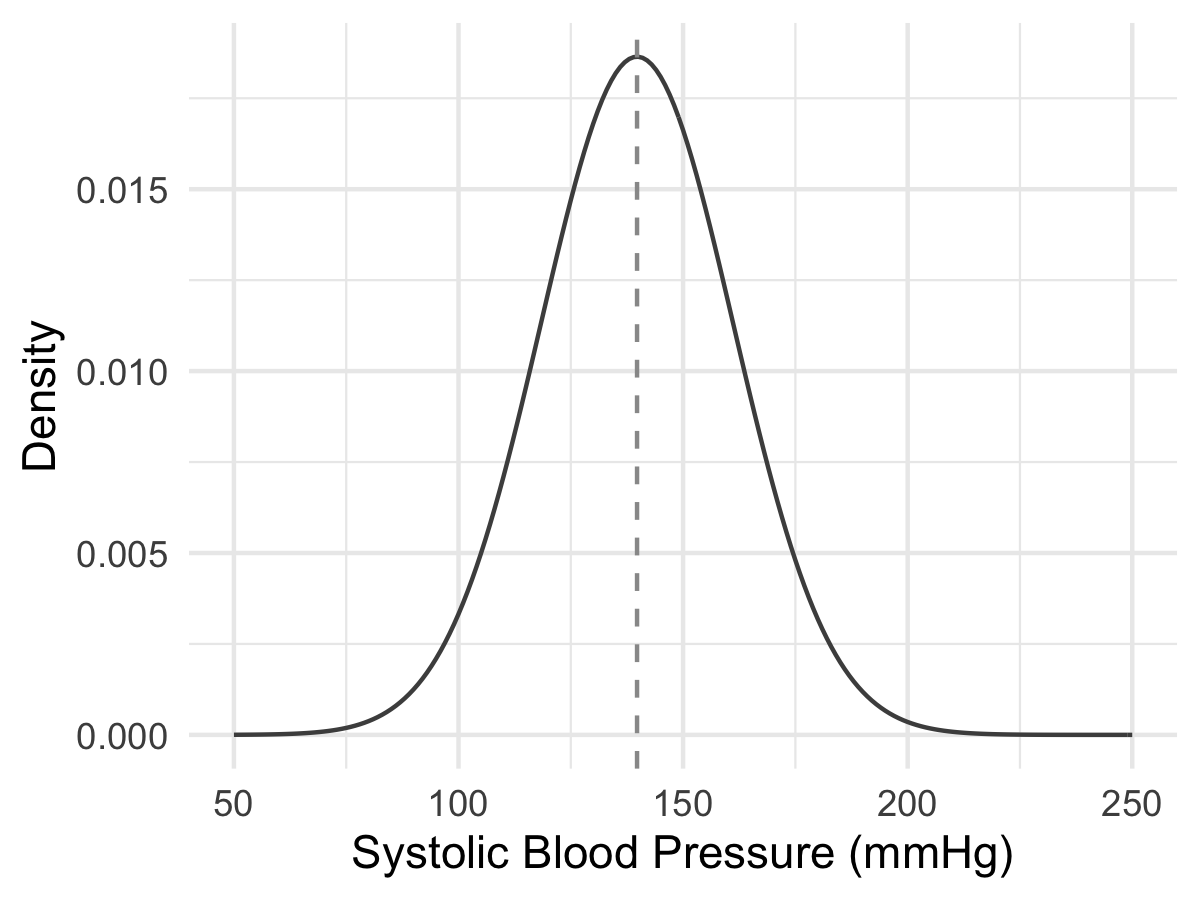
\includegraphics[width=0.7\textwidth]{img/hyp-z-test-example-00.png}
\end{center}

Here is a histogram of 10,000 data samples drawn independently from that distribution (i.e., what we would expect if we sampled the SBPs of 10,000 men from the United States at large):

\begin{center}
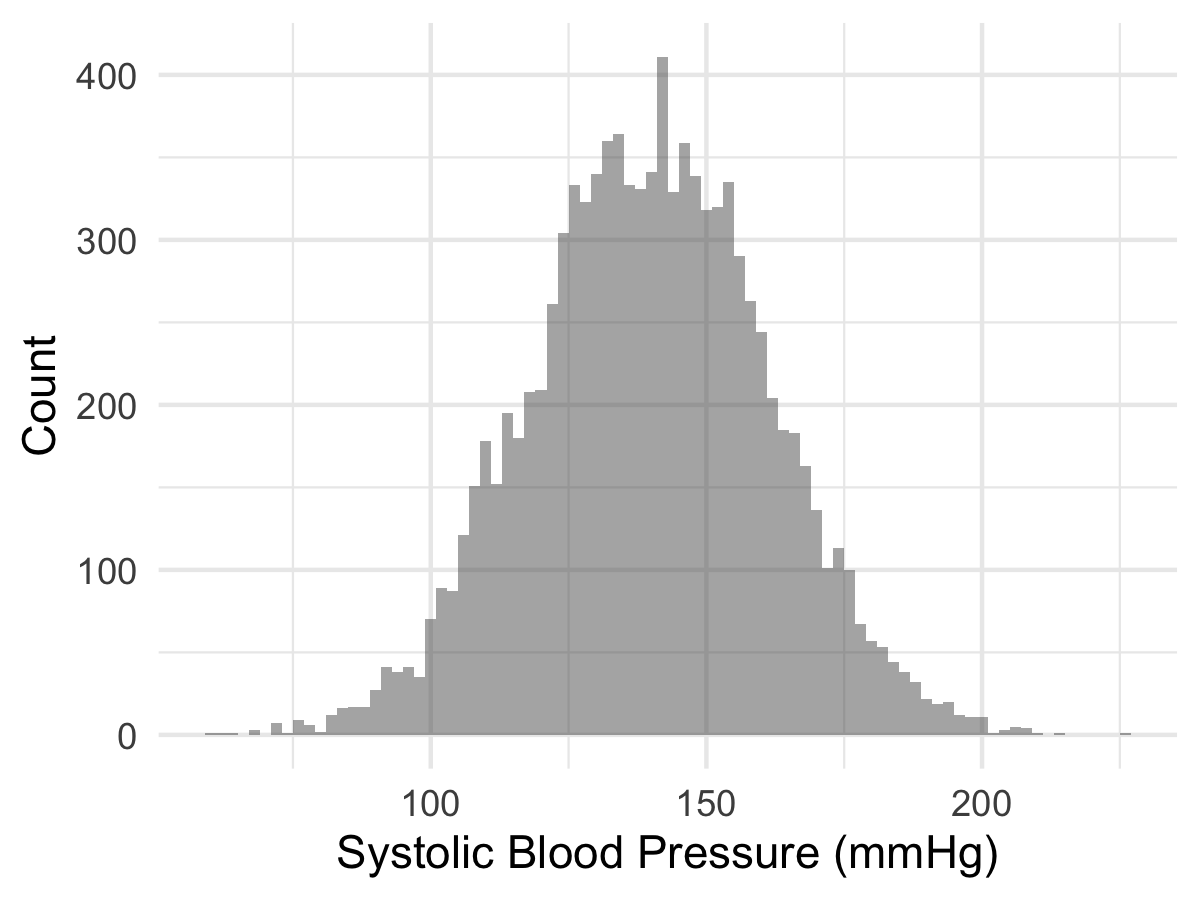
\includegraphics[width=0.7\textwidth]{img/hyp-z-test-example-0.png}
\end{center}

Now, assume some researchers find a small community in rural Appalachia and measure the SBP of 20 Caucasian males ages 55-64 there. Their mean SBP is 125.45 mmHg, illustrated by the red dashed line in the graph below.

\begin{center}
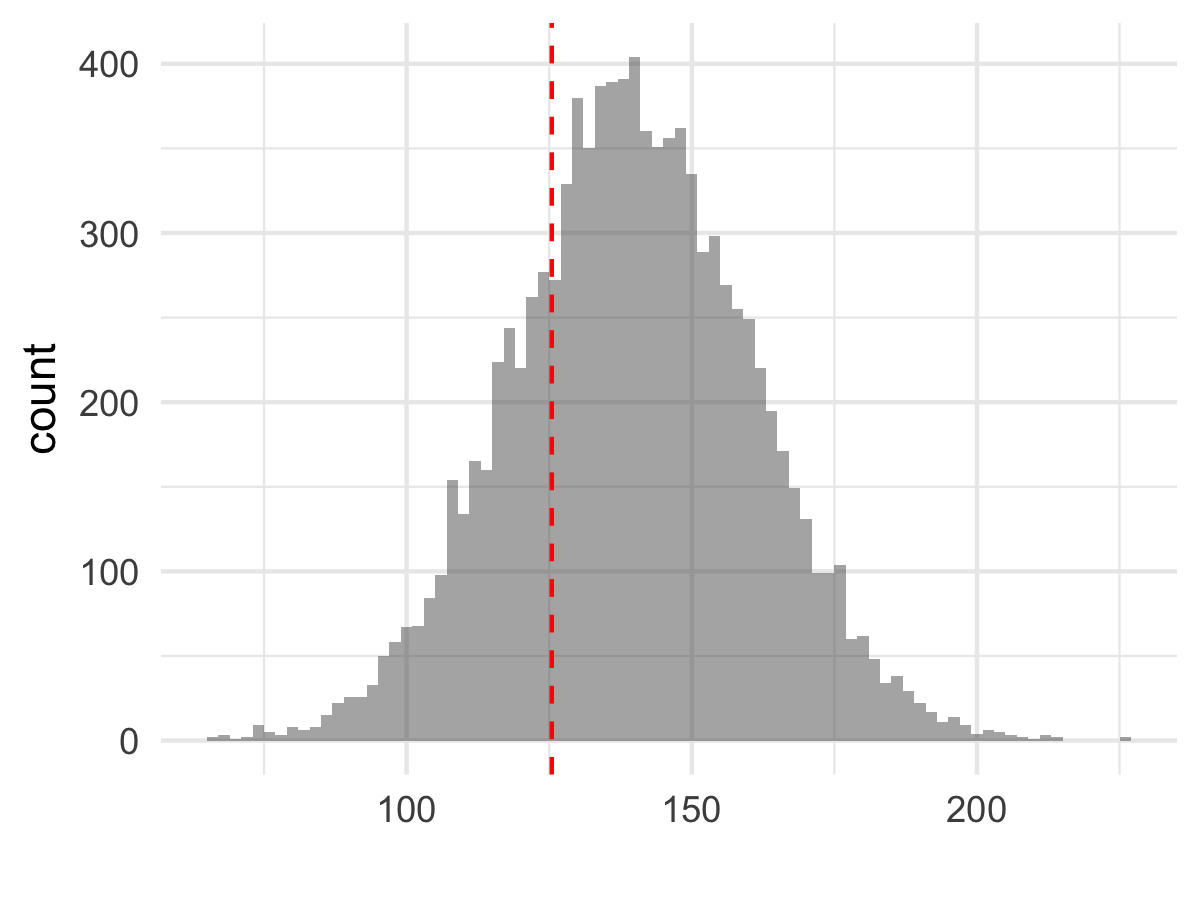
\includegraphics[width=0.7\textwidth]{img/hyp-z-test-example-1.png}
\end{center}

At first glance, this may not appear that unusual. After all, the red line is sort of near the center of the gray distribution, right? This analysis is flawed, however, because our 125.45 mmHg value isn't for one man - it's an average over 20 men. The distribution of the \textbf{sample mean}, $\overline{x}$, is different from that of each individual sample. 

To see this, imagine taking 20 samples from the gray distribution, taking their mean, and recording that value. Now repeat that process 10,000 times. If you do that, you get the \textbf{distribution of the sample mean},  which is skinnier than the gray distribution:
\begin{center}
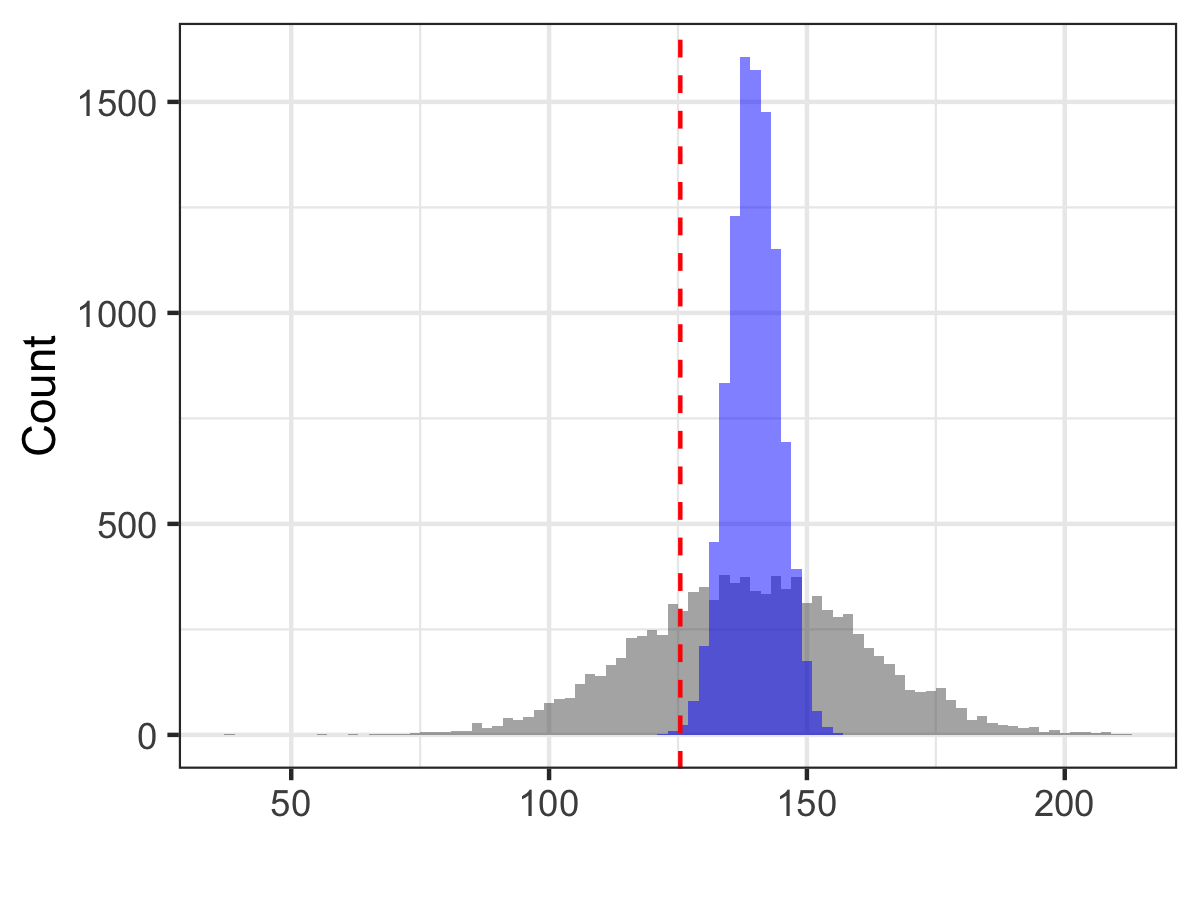
\includegraphics[width=0.7\textwidth]{img/hyp-z-test-example-2.png}
\end{center}
It turns out that the distribution of the sample mean will have the same mean, $\mu_0$, as the population distribution, but its standard deviation will be $\sigma/\sqrt{n}$, where $n$ is the number of samples over which the mean is taken.

\begin{question}{}
If $n=1$, what is the standard deviation of the sample mean? If $n=\infty$, what is the standard deviation of the sample mean?
\end{question}

\begin{question}{}
The sample mean for our $20$ sampled Appalachian men is shown as a vertical red dashed line in the figure above. Now that you know what the distribution of the sample mean looks like, do you think the observation from your Appalachian town is ``weird''?
\end{question}

\noindent Let's conduct a hypothesis test to evaluate whether we have evidence that the mean SBP among men in this town is different from that of the general U.S. population.

\begin{enumerate}
\item \textit{State the \textbf{null hypothesis}}. Here the null hypothesis is going to be our default position: that there is no difference. Let $\mu_c$ be the true mean SBP for men in the community and $\mu_0$ be the mean for the general population. 
\begin{align*}
H_0: &~\mu_c = \mu_0 \\
H_a: &~\mu_c \neq \mu_0
\end{align*}
\item \textit{List statistical {assumptions}}. We make two assumptions. First, we assume that the SBPs of the different men in the sample are statistically independent. Second, we assume that under the null, SBP will follow a normal distribution with mean 139.75 and standard deviation 21.40, the same as the general population of men aged 55-64.
\item \textit{Decide on an appropriate test and test statistic}. Our test statistic in this case is going to be the \textbf{Z-statistic}, which measures the deviation of the sample mean from the population mean in units of the standard deviation of the sample mean, $\sigma/\sqrt{n}$:
$$ Z = \frac{\overline{x} - \mu_0}{\sigma / \sqrt{n}} \qquad \text{where} \qquad \overline{x} = \frac{1}{n} \sum_{i=1}^n x^{(i)}$$
In our case, $n = 20$ because $\overline{x}$, our sample mean, is an average of 20 samples.  
\item \textit{Derive the distribution of the test statistic under the null}. The Z-statistic follows a \textbf{standard normal} distribution under the null, which is a normal distribution with $\mu=0$ and $\sigma=1$. To see this, remember that the distribution of $\overline{x}$ under the null is $\mathcal{N}(\mu_0, \sigma/\sqrt{n})$. When you calculate the Z-statistic, you shift that distribution by a distance $\mu_0$ so it is centered at zero, then adjust its width (standard deviation) to 1.0 by dividing by $\sigma/\sqrt{n}$.
\item \textit{Select a {significance level} under which you'll reject the null}. For the purposes of this example, we will choose $\alpha = 0.05$ (5\% chance of a type I error). The null distribution of the Z-statistic is shown below. The vertical dotted black lines are situated at the \textbf{critical values} that produce $\alpha = 0.05$ (the area under the null distribution that is outside those lines is 0.05). 

\begin{center}
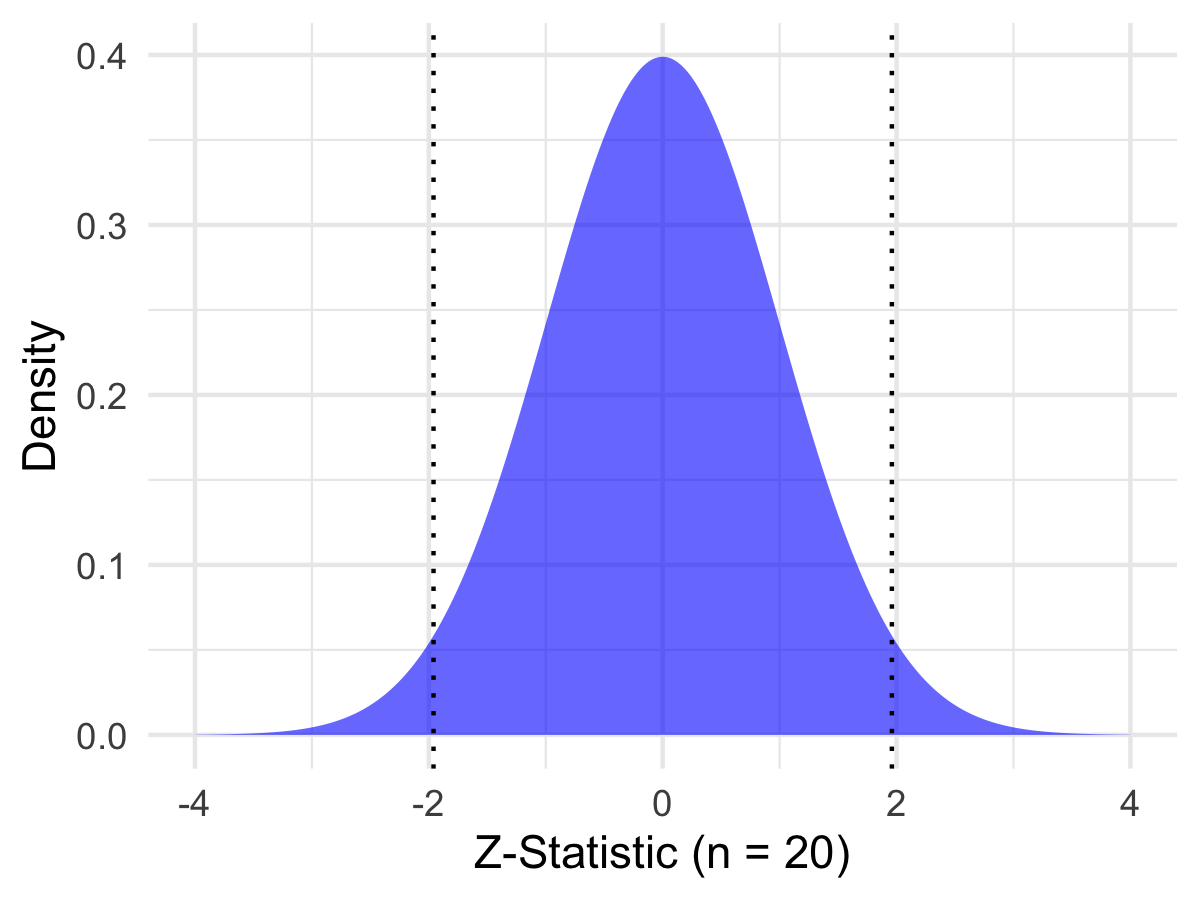
\includegraphics[width=0.7\textwidth]{img/hyp-z-test-example-3-z.png} 
\end{center}

\item \textit{Compute the observed value of the test statistic from the data.} The observed value of the test statistic is:
$$ Z = \frac{\overline{x} - \mu_0}{\sigma / \sqrt{n}} = \frac{125.45 - 139.75}{21.40/\sqrt{20}} = -2.99. $$
\item \textit{Decide whether or not to reject the null hypothesis.} The value of our test statistic falls outside the region contained by the critical values (the \textbf{acceptance region}), so we reject the null at this value of $\alpha$.
\begin{center}
\includegraphics[width=0.7\textwidth]{img/hyp-z-test-example-4-z.png} 
\end{center}
\end{enumerate}

\begin{question}{}
As $\alpha$ gets smaller, are you more or less likely to reject the null for the same value of the test statistic? Hint: What does making $\alpha$ smaller do to the positions of the two black dotted lines in the figure, above?
\end{question}

%%%%%%%%%%%%%%%%%%%%%%%%%%%%%%%%%%%%%%%%%%%%%%%%%%%%%%%%%%%%%%%%%%%%%%%%%%%%%%%%

\section{Definitions}

\begin{itemize}
\item \textbf{Type I Error:} When a hypothesis test rejects the null even though the null is true (also called a \textbf{false positive}). The type I error rate is usually denoted by $\alpha$.
\item \textbf{Type II Error:} When a hypothesis test fails to reject the null even though it is false (also called a \textbf{false negative}). The type II error rate is usually denoted by $\beta$.
\item \textbf{P-value:} The probability of obtaining a test statistic at least as extreme as the one that was actually obtained, assuming the null is true. A $p$-value can be \textbf{one-sided} or \textbf{two-sided}. The difference lies in the definition of ``extreme''. In a one-sided test, we find the probability that the test statistic is at least as extreme \emph{in the same direction} as the one we observed. In a two-sided test, we find the probability that the test statistic is at least as extreme \emph{in either direction} (positive or negative deviation). In most cases, this has the practical effect of doubling the $p$-value.
\item \textbf{Power:} The probability that a hypothesis test will reject the null when the null is false (that the test will detect a true effect if the effect is there). Usually denoted $1 - \beta$.
\end{itemize}

%%%%%%%%%%%%%%%%%%%%%%%%%%%%%%%%%%%%%%%%%%%%%%%%%%%%%%%%%%%%%%%%%%%%%%%%%%%%%%%%

\section{Pearson's Chi-Squared Test}

Imagine you have data on two discrete variables for $n$ different subjects. You want to test whether the value of one covariate is independent of the value of the other. To do this, you can arrange your data in a \textbf{contingency table} where the rows and columns correspond to the values of the two variables. \textbf{Pearson's chi-squared test} can then be used to assess the independence of row and column values.

\paragraph{Example: Association of Genotype and Disease} Imagine you want to test whether a person's genotype at a particular locus is associated with whether or not he/she has Disease X. You find 100 people with the disease and 100 healthy controls ($n=200$) and genotype them:

\begin{center}
\includegraphics[width=0.55\textwidth]{img/pearson-chisq-fig-1.png}
\end{center}

\noindent \noindent Let's conduct a hypothesis test to examine this result. 

\newcommand{\indep}{\perp \!\!\! \perp}
\newcommand{\independent}{\perp\mkern-9.5mu\perp}
\newcommand{\notindependent}{\centernot{\independent}}

\begin{enumerate}
\item \textit{State the \textbf{null hypothesis}}. We consider the genotype at this locus, $G$, to be a random variable (see Chapter~\ref{chapter:probabilitydistributions}) with three possible outcomes: \emph{AA}, \emph{Aa}, and \emph{aa}. We likewise consider the patient's disease status, $D$, to be a random variable with two possible outcomes: disease or no disease. We state our null hypothesis mathematically as: 
\begin{align*}
H_0: &~ G \independent D \\
H_a: &~ G \notindependent D
\end{align*}
where the symbol $\independent$ refers to statistical independence of $G$ and $D$. We encountered statistical independence in our discussion of maximum likelihood in Chapter~\ref{chapter:mlebasics}. Mathematically, statistical independence means that the joint probability of observing a particular value for $G$ and a particular value for $D$ is simply equal to the product of their individual probabilities:
$$ P(G=g, D=d) = P(G=g) P(D=d) $$
Under these conditions, the expected values of the cells of our table are:
\begin{center}
\includegraphics[width=0.55\textwidth]{img/pearson-chisq-fig-2.png}
\end{center}
For example, consider the cell $G = AA, D = X$. Assuming the total number of patients is fixed at $n=200$ and $G$ and $D$ are independent, the expected number of people in that cell is: 
\begin{align*} P(G=AA, D=X) \cdot n &= \left(\frac{119}{200}\right) \left(\frac{100}{200}\right) \cdot 200 \\
&= \mathbf{59.5} \end{align*}
Our task now is to decide whether our observed table counts are different enough from what we expect under the null to cause us to reject the null. 

\item \textit{List statistical {assumptions}}. We assume that the data are sampled randomly and independently from a fixed population where each member of the population has an equal probability of selection\footnote{A further assumption of the chi-squared test is that expected counts for each cell must be sufficiently high. A common rule is 5 or more in all cells of a $2\times 2$ table, and 5 or more in 80\% of cells in larger tables, but no cells with zero counts.}. 

\item \textit{Decide on an appropriate test and test statistic}. The chi-squared test works by calculating expected counts in all $r \times c$ cells of the table ($r$ = number of rows, $c$ = number of columns) and then measuring the data's deviation from those expected counts. The \textbf{chi-squared test statistic} has the form
$$ X^2 = \sum_{i=1}^r \sum_{j=1}^c \frac{(O_{ij} - E_{ij})^2}{E_{ij}} $$
where $O$ refers to ``observed count'' and $E$ to ``expected count''. The expected counts are those that assume statistical independence of rows and columns (blue table, above).

\item \textit{Derive the distribution of the test statistic under the null}. Under the null, the $X^2$ test statistic follows a chi-squared distribution (Section~\ref{sect:chisqdist}) with $(r-1)(c-1)$ degrees of freedom. In the case of our genotype example, there are $r=2$ rows and $c=3$ columns, thus $2$ degrees of freedom.

\item \textit{Select a {significance level} under which you'll reject the null}. The $\chi^2$ distribution with $2$ degrees of freedom is shown below. Two vertical lines are shown at different significance levels: $\alpha = 0.05$ and $\alpha = 0.1$.

\begin{center}
\includegraphics[width=0.6\textwidth]{img/hyp-chisq-test-example-2.png} 
\end{center}

\item \textit{Compute the observed value of the test statistic from the data.}

\begin{question}{}
Using the formula in step~$4$, above, compute the actual value of the chi-squared test statistic for this example. Hint: You should end up with a value that corresponds to the position of the red dashed line in the figure below. 
\begin{center}
\includegraphics[width=0.7\textwidth]{img/hyp-chisq-test-example-3.png} 
\end{center}
\end{question}

\item \textit{Decide whether or not to reject the null hypothesis.} Based on our calculated value of the test statistic, we will reject the null at $\alpha = 0.1$ and fail to reject the null at $\alpha = 0.05$.
\end{enumerate}

Although it looks much different from the Z-test, the chi-squared test follows the same formalism: defining a null hypothesis, figuring out what the data should look like under the null, quantifying the deviation of the observed data from what's expected using a test statistic, and deciding if that test statistic presents strong enough evidence to cause us to reject the null.  

%%%%%%%%%%%%%%%%%%%%%%%%%%%%%%%%%%%%%%%%%%%%%%%%%%%%%%%%%%%%%%%%%%%%%%%%%%%%%%%%%%%%%%

\section{Student's T-tests}

The final example we will look at today is the \textbf{T-test}. Like the $Z$-test, the $T$-test (actually a family of tests) deals with situations where you have data that are assumed to be normally distributed under the null hypothesis. However, in this scenario, the population standard deviation, $\sigma$ is not known and must be estimated from the data itself.

\subsection{One Sample T-test}

Assume you have a dataset $x^{(1)}, \dots, x^{(n)}$, of real numbers that you can plausibly assume are normally distributed. You want to test whether the mean of your data is equal to a fixed value, $\mu_0$. Under the null hypothesis that the means are the same, the test statistic
$$ T = \frac{\overline{x} - \mu_0}{s/\sqrt{n}} $$
which we call a ``T statistic'', follows a T-distribution (Section~\ref{sect:tdist}) with $n-1$ degrees of freedom\footnote{A one-sample T-test looks a lot like a Z-test. However, because we use $s$ to estimate the population standard deviation from data, we must account for variation in our estimate. It turns out that the sample variance, $s^2$, follows a chi-squared distribution with $n-1$ degrees of freedom, where $n$ is the sample size. In this case, by the definition of the $T$-distribution (Section~\ref{sect:tdist}), the T statistic follows a Student's T-distribution with $n-1$ degrees of freedom. As the number of samples, $n$, grows, the sample standard deviation approaches the population standard deviation and the T-test becomes a Z-test. But when $n$ is small, the T-test is quite a bit more conservative.}. Here $\overline{x}$ refers to the sample mean, and $s$ refers to the \textbf{sample standard deviation}:
$$ s = \sqrt{\frac{1}{n-1} \sum_{i=1}^n (x^{(i)} - \overline{x})^2} $$

\begin{question}{}
Compare the formula for the sample standard deviation to the maximum likelihood estimate of the parameter, $\sigma$, of a normal distribution (Section~\ref{sect:mlenormal}). What is the same/different? Note in particular the use of $n-1$ in the denominator, rather than $n$. This arises because the MLE for $\sigma$, $\hat{\sigma}$, is a \textbf{biased} estimate of the population standard deviation (more on this later). For large $n$, however, the two are nearly identical. 
\end{question}

\subsection{Two Independent Samples, Equal Variance}

Assume you have a dataset $x^{(1)}, \dots, x^{(n)}$ and another dataset $y^{(1)}, \dots, y^{(m)}$. You assume that both are drawn from normal distributions with equal variance but potentially different means. You want to test whether the means are equal. 

The same basic machinery for the one-sample T-test can be deployed in this context with a slightly different test statistic. The test statistic
$$ T = \frac{\overline{x} - \overline{y}}{s_p \sqrt{\cfrac{1}{n} + \cfrac{1}{m}}} $$
where
\begin{align*} s_p^2 &= \frac{(n-1) s_x^2 + (m-1) s_y^2}{m + n - 2} \\
s_x^2 &= \frac{1}{n-1} \sum_{i=1}^n (x^{(i)} - \overline{x})^2 \\
s_y^2 &= \frac{1}{m-1} \sum_{i=1}^m (y^{(i)} - \overline{y})^2 \end{align*}
follows a $t$-distribution with $m + n - 2$ degrees of freedom.

\subsection{Two Independent Samples, Unequal Variance}

Sometimes you have two independent samples but cannot assume the variances are equal. Again, similar machinery can be deployed. In this case, you can use \textbf{Welch's T-test}, which uses the test statistic
$$ T = \frac{\overline{x} - \overline{y}}{s_{xy}} $$
where 
$$ s_{xy} = \sqrt{\frac{s_x^2}{n} + \frac{s_y^2}{m}}. $$
This test statistic approximately follows a $t$-distribution with degrees of freedom given by the {Welch-Sattherwaite Equation}
$$ \text{d.f.} = \frac{\left(\cfrac{s_x^2}{n} + \cfrac{s_y^2}{m} \right)^2}{\cfrac{(s_x^2/n)^2}{n-1} + \cfrac{(s_y^2/m)^2}{m-1}} $$ 

\subsection{Matched Pairs}

Assume you have a data set of matched pairs. This could be a set of measurements of the same individuals taken at two different points in time, for example, or paired measurements taken from individuals with similar characteristics. You want to test whether the second set of values have changed relative to the first set of values.

To do this, you can use a one-sample T-test on the \emph{differences} of the individual pairs. If no change has occurred, you would expect the mean of those differences to be zero. If we define $x^{(i)}$ as the difference of the paired observations for sample $i$ and $\overline{x}$ as $\frac{1}{n}\sum_{i=1}^n x^{(i)}$, the sample mean of those differences, then

$$ T = \frac{\overline{x}}{s/\sqrt{n}}$$

\noindent follows a T-distribution with $n-1$ degrees of freedom. 

\begin{question}{}
Here are some sample data. They come from a study that looked at the effect of ozone, a component of smog, on the weight gain of rats. (Original source: Biometrika 63: 421-434, 1976, reproduced in Rice's \emph{Mathematical Statistics and Data Analysis}, p. 465.) A group of 22 seventy-day-old rats were kept in an environment containing ozone for $7$ days, and their weight gains were recorded. Another group of 23 rats of a similar age were kept in an ozone-free environment for a similar time and their weight gains were also recorded. Here are the data for the control group:

{\footnotesize \tt
\begin{center}
\begin{tabular}{rlrr}
  \toprule
  & group & original\_weight & weight\_gain \\ 
  \midrule
  1 & control & 340.8 & 41.0 \\ 
  2 & control & 389.1 & 25.9 \\ 
  3 & control & 355.2 & 13.1 \\ 
  4 & control & 421.8 & -16.9 \\ 
  5 & control & 377.1 & 15.4 \\ 
  6 & control & 404.3 & 22.4 \\ 
  7 & control & 321.2 & 29.4 \\ 
  8 & control & 447.5 & 26.0 \\ 
  9 & control & 305.9 & 38.4 \\ 
  10 & control & 335.9 & 21.9 \\ 
  11 & control & 386.3 & 27.3 \\ 
  12 & control & 377.0 & 17.4 \\ 
  13 & control & 357.2 & 27.4 \\ 
  14 & control & 441.7 & 17.7 \\ 
  15 & control & 383.7 & 21.4 \\ 
  16 & control & 373.7 & 26.6 \\ 
  17 & control & 336.0 & 24.9 \\ 
  18 & control & 419.4 & 18.3 \\ 
  19 & control & 287.1 & 28.5 \\ 
  20 & control & 602.8 & 21.8 \\ 
  21 & control & 325.4 & 19.2 \\ 
  22 & control & 452.4 & 26.0 \\ 
  23 & control & 398.9 & 22.7 \\ 
  \midrule
  Mean & control & 384.4 & 22.4 \\
  St.Dev. & control & 65.5 & 10.8 \\
  \bottomrule
\end{tabular}
\end{center}
}

\noindent And here are the data for the ozone group:

{\footnotesize \tt
\begin{center}
\begin{tabular}{rlrr}
  \toprule
  & group & original\_weight & weight\_gain \\ 
  \midrule
  1 & ozone & 437.4 & 10.1 \\ 
  2 & ozone & 275.9 & 7.3 \\ 
  3 & ozone & 296.3 & -9.9 \\ 
  4 & ozone & 295.9 & 17.9 \\ 
  5 & ozone & 379.7 & 6.6 \\ 
  6 & ozone & 274.1 & 39.9 \\ 
  7 & ozone & 360.0 & -14.7 \\ 
  8 & ozone & 331.9 & -9.0 \\ 
  9 & ozone & 531.8 & 6.1 \\ 
  10 & ozone & 350.5 & 14.3 \\ 
  11 & ozone & 345.7 & 6.8 \\ 
  12 & ozone & 268.1 & -12.9 \\ 
  13 & ozone & 339.9 & 12.1 \\ 
  14 & ozone & 352.4 & -15.9 \\ 
  15 & ozone & 435.8 & 44.1 \\ 
  16 & ozone & 476.9 & 20.4 \\ 
  17 & ozone & 462.5 & 15.5 \\ 
  18 & ozone & 368.0 & 28.2 \\ 
  19 & ozone & 504.3 & 14.0 \\ 
  20 & ozone & 188.0 & 15.7 \\ 
  21 & ozone & 466.9 & 54.6 \\ 
  22 & ozone & 288.8 & -9.0 \\ 
  \midrule
  Mean & ozone & 365.0 & 11.0 \\
  St.Dev. & ozone & 88.6 & 19.0 \\
  \bottomrule
\end{tabular}
\end{center}
}

\begin{enumerate}
\item[(a)] Imagine that the population weight distribution of rats is known to be normal with $\mu = 350$ (grams) and unknown $\sigma$. How would you test the hypothesis that the mean of the control group is equal to the population mean? How would you test the hypothesis that the mean of the ozone group is equal to the population mean?
\item[(b)] How would you test the hypothesis that the mean original weights of the ozone and control groups are equal? Do not assume equal variance. 
\item[(c)] How would you test the hypothesis that the mean weight gain in the ozone group is equal to the mean weight gain in the control group? Do not assume equal variance.
\item[(d)] How would your approach in part (c) change if you assumed the weight gains in the two groups had equal variance?
\end{enumerate}

\noindent Plug in the relevant numbers from the tables above to perform each hypothesis test with $\alpha = 0.05$. The following table of critical values for the $T$-distribution\footnote{Borrowed with gratitude from https://www.stat.purdue.edu/~lfindsen/stat503/t-Dist.pdf} may help you:

\begin{center}
\includegraphics[width=0.9\textwidth]{img/t-distribution-critical-values.png}
\end{center}

\noindent \textbf{Answers:} (a) One-sample $T$-test of control group original weights vs. null of $\mu_0 = 350$; $T$-statistic is 2.5165, 22 d.f., two-sided $p$-value is 0.01964, reject null at $\alpha=0.05$. One-sample $T$-test of ozone group original weights vs. null of $\mu_0 = 350$; $T$-statistic is 0.7961, 21 d.f., two-sided $p$-value is 0.4349, fail to reject null at $\alpha=0.05$. (b) Welch's two-sample $T$-test of control vs. ozone group original weights; $T$-statistic is 0.8293, d.f is estimated using the Welch-Sattherwaite equation at 38.619, two-sided $p$-value is 0.4120, fail to reject null at $\alpha=0.05$. (c) Welch's two-sample $T$-test of control vs. ozone group weight gains; $T$-statistic is 2.4629, d.f. is estimated using the Welch-Sattherwaite equation at 32.918, two-sided $p$-value is 0.01918, reject null at $\alpha=0.05$. (d) You would use Pearson's two-sample $T$-test, which assumes equal variances; $T$-statistic is 2.4919, d.f. is 43, two-sided $p$-value is 0.01664, reject null at $\alpha=0.05$. 

\end{question}

% %%%%%%%%%%%%%%%%%%%%%%%%%%%%%%%%%%%%%%%%%%%%%%%%%%%%%%%%%%%%%%%%%%%%%%%%%%%%%%%%

\section{Statistical Power}

\textbf{Power} is the probability that a hypothesis test will reject the null hypothesis if the alternative hypothesis is, in fact, true. The graph below shows two distributions: the sampling distribution under the null (mean $\mu_0$) and the sampling distribution under the alternative hypothesis (mean $\mu_1$). Note that these sampling distributions are for the \emph{test statistic}; it could be the sample mean, sample proportion, sample correlation coefficient, sample difference in means, etc.

\begin{center}
\includegraphics[width=0.65\textwidth]{img/statistical-power-chart.png}
\end{center}

\begin{mdframed}
\textbf{Question 2.8:} There are three ways to increase the power of a hypothesis test. (Hint: Have a look at the parameters in the formula for the $T$-test statistic, above.) Try to list them here:
\begin{enumerate}
\item ~
\item ~
\item ~
\end{enumerate}
\vspace{5mm}
\end{mdframed}

%%%%%%%%%%%%%%%%%%%%%%%%%%%%%%%%%%%%%%%%%%%%%%%%%%%%%%%%%%%%%%%%%%%%%%%%%%%%%%%%

\section{Sample Size Calculations}

For many statistical hypothesis tests, we can reverse the calculation and ask: how many samples do we need at a certain effect size to reject the null at a given significance level? Even in cases where you can't invert the test statistic itself, you can often use \textbf{bootstrapping}, \textbf{permutations}, etc. to simulate the appearance of the data under the null. 

This graph shows the number of samples required to detect the effect size shown in the Appalachian town example in the slides ($\overline{x} = 125.45$, $\mu_0 = 139.75$) at varying significance levels: $\alpha = 0.1$ (orange line), $\alpha = 0.05$ (blue dotted line), and $\alpha = 0.01$ (turquoise dashed line). 

\begin{center}
\includegraphics[width=0.5\textwidth]{img/hyp-z-test-power-curve-1.png}
\end{center}

Now let's vary the effect size. The graph below shows three lines, representing the sample sizes needed to reject the null at $\alpha = 0.1$ (solid), $0.05$ (dotted), and $0.01$ (dashed) significance levels, using a two-sided test.

\begin{center}
\includegraphics[width=0.5\textwidth]{img/hyp-z-test-power-curve-2.png}
\end{center}

\chapter{Decision Trees {\color{red} DRAFT} \label{chapter:decisiontrees}}

{\bf Decision trees} were developed as an alternative to neural networks in the 1970s. They can be used either for classification or regression. There are several algorithms for fitting decision trees, all of which are heuristic, because the general problem of learning an optimal decision tree for a dataset is NP-complete. All algorithms for tree learning are \textbf{greedy} and are not guaranteed to give the optimal solution.

\subsection{Entropy and Information Gain}

Today we will discuss the ID3 algorithm for building decision trees, which relies on the concepts of entropy and information gain. \textbf{Entropy}, usually abbreviated $H$, is a measure of the uncertainty in the value of a random variable. It is the number of bits (on average) required to describe the outcome of the random variable. Here is the formula for the entropy of the discrete probability distribution governing the outcome of a random variable, $X$:

$$ H(X) = - \sum_{x} P(X = x) \log_2\left(P(X = x)\right) $$

For a Bernoulli random variable, there are only two possible outcomes: 0 and 1. The entropy of this random variable is given by:

$$ H_\text{Bernoulli} = -\mu \log_2(\mu) - (1 - \mu) \log_2 (1 - \mu) $$

where $\mu$, as usual, is the probability the outcome is 1. 

Let $Y$ be the outcome variable of a training set. Let $X$ be some other random variable defined over the training set. It could be one of the original predictors or some arbitrary combination of them. \textbf{Information gain} is defined as:
\begin{align*} \text{Gain}(Y, X) &= H(Y) - \sum_{x} P(X = x)~ H(Y|X=x) \\
&= H(Y) - H(Y|X) \end{align*}
It is a measure of how much our uncertainty in the value of $Y$ is reduced by knowing $X$. 

\subsection{The ID3 Algorithm}

Here is the algorithm:
\begin{enumerate}
\item Start with a single node representing the entire dataset.
\item At each current leaf node in the tree:
\begin{enumerate}
\item Compute the information gain for each feature in turn.
\item Split on the one with the highest information gain.
\end{enumerate}
\item Return to Step 2. Stop the recursion when either the class distributions at the leaf nodes are entirely pure (all data points at a leaf have the same outcome class), or there are no more variables left to split on.
\end{enumerate}

\subsection{Decision Tree Regression}

So far we've assumed that our outcome is discrete. But what happens if it's numeric? (That is, what if we want to perform regression instead of classification?)

In that case, we use \textbf{standard deviation reduction} instead of information gain to decide which variables to split on. The sample standard deviation of an outcome, $y$, is defined as:

$$ S(Y) = \sqrt{\frac{\sum_i(y^{(i)} - \overline{y})}{n-1}} $$

The procedure is identical to the ID3 algorithm except you use conditional standard deviation instead of information gain to decide on features. We define

$$ S(Y, X) = \sum_{x} P(X = x)~ S(Y(X=x)) $$

and at each current leaf node, we split on the variable where the reduction in standard deviation, $S(Y) - S(Y,X)$, is the highest. 

\subsection{Numeric Predictors}

So far we've also assumed that our predictors are discrete. But decision trees can handle numeric predictors as well. There are many different strategies for deciding on an optimal split for a predictor. Two simple ones:

\begin{itemize}
\item Split at the median or mean of the predictor.
\item Order the datapoints on the value of the predictor and consider each possible split, looking for the one that gives the greatest information gain/standard deviation reduction. So for example, if you have a predictor called ``age'' and its values are $10, 11, 16, 18, 20$, and $35$, consider all $N-1 = 5$ possible split points. (This is the approach used by C4.5, a successor to ID3.) 
\end{itemize}

If you have a large dataset, the second option is probably not practical, but you can downsample your dataset first and then look for the optimal cut point(s).


%\chapter{Distance Metrics \label{chapter:distancemetrics}}


\chapter{Model Complexity and the Bias-Variance Tradeoff \label{chapter:biasvariance}}

In classification, \textbf{model complexity} (i.e. the effective number of parameters the model must fit) is typically related to the intricacy and complexity of the decision boundary; the more parameters in the model, the more complex the boundary.

\section{Goodness of Fit vs. Generalizability}

Training vs. test error

\section{Bias vs. Variance}

This figure shows the training and test error for KNN as a function of $K$ for a classification example similar to the one discussed in Chapter~\ref{chapter:classification}, as well as the training and test error for a linear model (which doesn't vary with $K$). You can see that the curves have characteristic shapes that vary with $K$. It turns out these shapes reflect a general principle for all supervised learning called the \textbf{bias-variance tradeoff}. 

The bias-variance tradeoff: KNN example. The Bayes error rate, or \textbf{irreducible error}, is the probability an instance is misclassified by a classifier that knows the true class probabilities given the predictors. From \emph{Elements of Statistical Learning}, Figure 2.4.

\begin{center}
\includegraphics[width=0.8\textwidth]{img/l03-knn-linear-tradeoff.png}
\end{center}

Illustration of training vs. test error as a function of model complexity, as well as the bias-variance tradeoff. From \emph{Elements of Statistical Learning}, Figure 2.11.

\begin{center}
\includegraphics[width=0.8\textwidth]{img/l03-bias-variance-tradeoff.png}
\end{center}

A graphical illustration of the difference between bias and variance. Think of each dot as representing a single test example evaluated under the same model trained on slightly different datasets. The center of the target is the prediction the model should make for that test example. In the case of high bias and low variance, all of the models are off, but they are ``wrong in the same way''. If you average their predictions, the answer is still way off the mark. In the case of high variance, the models all make very different predictions on the same training example. However, their predictions are off in random directions from the center, so if you average their outputs, you'll get closer to the right answer. 

\begin{center}
\includegraphics[width=0.7\textwidth]{img/targets-bias-variance.png}
\end{center}

\section{Overfitting vs. Underfitting}

\begin{question}{}
What are the advantages and disadvantages of KNN with low $K$ (e.g. $K=3$) vs. high $K$ (e.g. $K=50$)? The decision boundaries for the previous example with (left to right) $K=3, 15,$ and $50$ are shown below.
\begin{center}
\includegraphics[width=0.3\textwidth]{img/esl-knn-3.png}
\includegraphics[width=0.3\textwidth]{img/esl-knn-15.png}
\includegraphics[width=0.3\textwidth]{img/esl-knn-50.png}
\end{center}
\end{question}

\begin{question}{}
We have discussed bias and variance in the context of classification (a yes/no outcome). How would training and test error, overfitting vs. underfitting, etc. be quantified if the outcome was a number, as in a regression problem (Chapter~\ref{chapter:regression})?
\end{question}

\chapter{Feature Engineering and Feature Selection \label{chapter:featureengineering}}

The methods we've studied in Chapters~\ref{chapter:classification} and \ref{chapter:regression}, as well as all other supervised (and unsupervised) machine learning algorithms, all depend on the concept of a \textbf{feature}. A feature is some aspect of each training example that the model designer believes will influence its relationship to the outcome, or that captures some aspect of the data in a way that is relevant to the problem he/she is trying to solve. 

Before any algorithm can be applied, therefore, it is necessary to decide how to represent the data: which features to include and how to extract them from the raw data. This task is called \textbf{feature engineering}. In most cases, the model designer will also want to incorporate some form of \textbf{feature selection}: a process that automatically or semi-automatically decides which features are most relevant to the model and discards the others.

\vspace{5mm}

\begin{question}{}
Choose 2-3 examples from the list of problems in Section~\ref{section:projectexamples}. Describe the setup of each problem and what types of features one would need to collect to build an accurate/useful model. 
\end{question}

%%%%%%%%%%%%%%%%%%%%%%%%%%%%%%%%%%%%%%%%%%%%%%%%%%%%%%%%%%%%%%%%%%%%%%

\section{Sample Dataset}

The so-called ``Pima Indians diabetes dataset'' was collected in the 1980s. It includes information on 768 women from the Pima people, who live near Phoenix, Arizona. The Pima were, as of the late 1980s, under continuous study by the National Institute of Diabetes and Digestive and Kidney Diseases because of their high incidence of diabetes\footnote{The causative factors behind this high diabetes rate are not clear. Some scholars believe that it was driven by a sudden shift in diet during the last century from traditional agricultural crops to processed foods, together with a decline in physical activity \cite{schulz2006effects}.}. There are eight predictors in the dataset and one outcome. The predictors are:
\begin{center}
\texttt{ \small
\begin{tabular}{lp{0.6\textwidth}}
\toprule
Predictor & Description \\
\midrule
Pregnancies & Number of times pregnant \\
Glucose & Plasma glucose concentration in a two-hour oral glucose tolerance test \\
BloodPressure & Diastolic blood pressure (mm Hg) \\
SkinThickness & Triceps skin fold thickness (mm) \\
Insulin & Two-hour serum insulin ($\mu$U/mL) \\
BMI & Body mass index (weight in kg/(height in m)$^2$) \\
DiabetesPedigreeFunction & Diabetes pedigree function (developed by research team; described in paper) \\
Age & Age in years \\
\bottomrule
\end{tabular}
}
\end{center}

The outcome is whether or not the woman went on to develop type II diabetes within $5$~years from the time of the survey. 

\begin{question}{}
Why is coding this outcome as 0/1, or yes/no, potentially problematic?
\end{question}

\begin{question}{}
What type of problem is this? What methods should we consider when solving this problem? Name at least three learning algorithms that might be appropriate. 
\end{question}

%%%%%%%%%%%%%%%%%%%%%%%%%%%%%%%%%%%%%%%%%%%%%%%%%%%%%%%%%%%%%%%%%%%%%%

\section{Feature Engineering}

Feature engineering mostly depends on domain expertise. There are three major analytical considerations when performing feature engineering: how the raw data is represented/summarized into features, how those features enter the model (e.g., do they need to be transformed or combined), and how different features are related to each other. 

\subsection{Representation}

Rarely will raw data, especially observational data, feed directly into a model. More often, one must decide how to design features that capture aspects of the data that are likely to be important to the model. 

\vspace{2mm}

\begin{question}{}
These histograms show the distributions of the individual predictors in the Pima dataset. In each case, what is one alternative way that the same information could be represented as a feature? For predictors 2--6, what do you think the zero values mean and how should they be dealt with?
  \begin{enumerate}
  \item Pregnancies
    \begin{center}
    \includegraphics[width=0.65\textwidth]{img/pima-pregnancies.png}
    \end{center}
    \newpage
  \item Glucose
    \begin{center}
    \includegraphics[width=0.65\textwidth]{img/pima-glucose.png}
    \end{center}
  \item BloodPressure
    \begin{center}
    \includegraphics[width=0.65\textwidth]{img/pima-blood-pressure.png}
    \end{center}
  \item SkinThickness
    \begin{center}
    \includegraphics[width=0.65\textwidth]{img/pima-skin-thickness.png}
    \end{center}
    \newpage
  \item Insulin
    \begin{center}
    \includegraphics[width=0.65\textwidth]{img/pima-insulin.png}
    \end{center}
  \item BMI
    \begin{center}
    \includegraphics[width=0.65\textwidth]{img/pima-bmi.png}
    \end{center}
  \item DiabetesPedigreeFunction
    \begin{center}
    \includegraphics[width=0.65\textwidth]{img/pima-diab-ped-function.png}
    \end{center}
    \newpage
  \item Age
    \begin{center}
    \includegraphics[width=0.65\textwidth]{img/pima-age.png}
    \end{center}
  \end{enumerate}
\end{question}

\begin{question}{}
The type of study design here is called a \textbf{prospective cohort study}. How would you collect information on these eight predictors if this were a \textbf{retrospective cohort study} (e.g., if you collected information about these women and their subsequent development of diabetes from the EHR)? How might this change affect how you extract and code the predictors? 
\end{question}

\subsection{Transformations}

Depending on the learning algorithm you're using and the goal of your project, you may or may not decide to employ transformations. A \textbf{transformation} is simply the application of a deterministic mathematical function to your data. In a supervised learning problem, you can transform one or more of the predictors and/or the outcome. Transformations are used to improve the interpretability of the model and/or to ensure that the model fulfills the assumptions of the statistical inference method(s) being used (e.g., a hypothesis test).

For example, here is what happens to the ``diabetes pedigree function'' predictor in the Pima dataset when we employ a common transformation called a \textbf{log transformation}\footnote{Here we are using log base 10, but you could also perform a similar transformation with the natural log, $\log_2$, etc.}:

\begin{center}
\includegraphics[width=0.49\textwidth]{img/pima-diab-ped-function.png} \includegraphics[width=0.49\textwidth]{img/pima-diab-ped-function-log.png}
\end{center}

\begin{question}{}
In the log transformation shown here, we simply replace each value, $x$, by $\log_{10}(x)$. Every unit increase on a $\log_{10}$ scale corresponds to a 10-fold multiplication on the usual scale of the predictor. If you put the log-transformed predictor into a regression model in place of the original (linear is the easiest to understand, but you could also consider logistic, Poisson, etc.), how would that change your interpretation of the model? 
\end{question}

Political science, economics, sociology, and related disciplines, which are heavily dependent on the use of linear regression models and hypothesis tests, rely extensively on transformations. In my experience, machine learning folks spend almost no time on them because their primary concern is predictive accuracy, not model interpretation. Machine learning practitioners, however, very frequently \textbf{scale and center} their predictors (see footnote in Section~\ref{section:sehyp}), which is another type of transformation. We will get into more detail on transformations as we continue to learn about regression models. 

\subsection{Correlations and Redundancy \label{section:redund}}

Including dozens or hundreds of predictors in a model does not guarantee that each contributes independent information. A good rule of thumb for any model is that it should be \textbf{parsimonious}: it should accomplish its goal with as little complexity and as few parameters as possible.

Finding a parsimonious model often means identifying sources of redundancy in a dataset. Often, two or more variables will be \textbf{correlated}, meaning that the value of one provides at least some information about the value of the other(s). A good way to alert yourself to the presence of highly correlated predictors is to create some sort of \textbf{correlogram}, or scatterplot matrix, which looks at associations between all pairs of variables. A correlogram for the Pima dataset is below.

\begin{center}
\includegraphics[width=\textwidth]{img/pima-ggpairs.png}
\end{center}

\begin{question}{}
This correlogram quantifies correlation using a metric called the \textbf{Pearson correlation coefficient}. Which pairs of predictors are the most tightly correlated? Are they positively or negatively correlated? How might you modify your dataset to eliminate redundancies in the information contributed by the different predictors?
\end{question}

Including correlated predictors is not always a bad thing, especially if your goal is prediction rather than model interpretation (see \cite{guyon2003introduction}, Figures 1, 2, and 3). The presence of correlations will also affect different types of models in different ways, and some suffer more than others. 

For example, here are eight univariate logistic regression models that capture the effect of each predictor in the Pima dataset on the outcome of diabetes vs. no diabetes:

\begin{center}
\includegraphics[width=0.45\textwidth]{img/cor-example-pregnancies.png}
\includegraphics[width=0.45\textwidth]{img/cor-example-glucose.png} \\[2mm]
\includegraphics[width=0.45\textwidth]{img/cor-example-bp.png}
\includegraphics[width=0.45\textwidth]{img/cor-example-skin-thickness.png} \\[2mm]
\includegraphics[width=0.45\textwidth]{img/cor-example-insulin.png}
\includegraphics[width=0.45\textwidth]{img/cor-example-bmi.png} \\[2mm]
\includegraphics[width=0.45\textwidth]{img/cor-example-diab-ped-funct.png}
\includegraphics[width=0.45\textwidth]{img/cor-example-age.png}
\end{center}

The coefficients on each predictor here are called the \textbf{unadjusted coefficients}, and the p-values on the predictor-specific hypothesis tests are called  \textbf{unadjusted p-values}. If you exponentiate a coefficient in a univariate logistic regression model, you get an \textbf{unadjusted odds ratio}\footnote{See Chapter~\ref{chapter:glms} if you don't understand why you're exponentiating or where the term ``odds ratio'' comes from. The odds ratio compares the odds of having a positive outcome among two groups separated by a one unit difference of the predictor in question, all else being the same.}. Here is a summary table:
\vspace{-3mm}

\begin{center} 
\texttt{ \small
\begin{tabular}{llll}
\toprule
Predictor & Unadjusted  & Unadjusted  & Unadjusted  \\
& Coefficient & Odds Ratio & P-value \\
\midrule
Pregnancies & 0.137 & 1.147 & $<$0.001 \\
Glucose & 0.038 & 1.039 & $<$0.001 \\
BloodPressure & 0.007 & 1.007 & 0.073 \\
SkinThickness & 0.010 & 1.010 & 0.039 \\
Insulin & 0.002 & 1.002 & $<$0.001 \\
BMI & 0.094 & 1.100 & $<$0.001 \\
DiabetesPedigreeFunction & 1.083 & 2.953 & $<$0.001 \\
Age & 0.042 & 1.043 & $<$0.001 \\
\bottomrule
\end{tabular}
}
\end{center}

Now let's create one big logistic regression model that includes all eight predictors. This is called a \textbf{multivariate} model. The coefficients, exponentiated coefficients, and p-values are often called \textbf{adjusted} in this case, or one might say that the odds ratio measures the effect of one predictor, \textbf{controlling for} the effects of the other predictors. Here are the adjusted estimates:
\vspace{-3mm}
\begin{center} 
\texttt{ \small
\begin{tabular}{llll}
\toprule
Predictor & Adjusted  & Adjusted  & Adjusted  \\
& Coefficient & Odds Ratio & P-value \\
\midrule
Pregnancies & 0.123 & 1.131 & $<$0.001 \\
Glucose & 0.035 & 1.036 & $<$0.001 \\
BloodPressure & -0.013 & 0.987 & 0.011 \\
SkinThickness & 0.001 & 1.001 & 0.929 \\
Insulin & -0.001 & 0.999 & 0.186 \\
BMI & 0.090 & 1.094 & $<$0.001 \\
DiabetesPedigreeFunction & 0.945 & 2.573 & 0.002 \\
Age & 0.015 & 1.015 & 0.111 \\
\bottomrule
\end{tabular}
}
\end{center}

\begin{question}{}
How can the odds ratio for Insulin be so close to 1.0 yet its p-value so low? (Hint: See Section~\ref{section:sehyp}.)
\end{question}

\begin{question}{}
Why might the coefficient and p-value for SkinThickness change so much in the shift from unadjusted to adjusted? 
\end{question}


%%%%%%%%%%%%%%%%%%%%%%%%%%%%%%%%%%%%%%%%%%%%%%%%%%%%%%%%%%%%%%%%%%%%%%

\section{Feature Selection}

The process of feature selection is largely about eliminating redundancies and useless predictors in an effort to come up with the most parsimonious model possible. In many cases, it is also about increasing the accuracy of model interpretation. There are three basic approaches to feature selection: filters, wrappers, and embedded methods. 

\subsection{Filters}

\textbf{Filter methods} select subsets of variables as a preprocessing step, \emph{independently of the chosen model}. These methods use \textbf{proxy measures} to rank variables; the proxy measure is often chosen to be computationally fast so that large numbers of features can be sifted through quickly.

A predetermined threshold of the proxy measure is usually used to determine which features pass to the multivariate modeling stage. Alternatively, the modeler may decide on a fixed number of features to include. Some examples of filter methods include:

\begin{itemize}
\item Any kind of univariate model (e.g. univariate logistic or linear regression)
\item Any kind of hypothesis test (e.g. t-test, chi-squared test; see Chapter~\ref{chapter:hypothesistesting})
\item Any kind of correlation coefficient (e.g. Pearson, Spearman)
\item Mutual information\footnote{The mutual information, in another format, is the most common splitting criterion used for decision trees; see Chapter~\ref{chapter:decisiontrees}. In the case of continuous variables, the sums are replaced by integrals.} 
$$ MI(X_i,Y) = \sum_x \sum_y P(X_i = x, Y = y) \log \frac{P(X_i = x, Y = y)}{P(X_i = x) P(Y = y)} $$
\item Variance thresholding (simply remove features with low variance)
\end{itemize}

\begin{question}{}
If you wanted to use the univariate logistic regression models above in Section~\ref{section:redund} as a filter for a downstream model (potentially not even multivariate logistic regression - it could be a decision tree, etc.), how would you rank them and how would you decide on an appropriate cutoff? 
\end{question}

\begin{question}{}
How would you apply a filter-based selection method in a case where you had dozens of different predictors of different types (e.g. some categorical, some binary, some numeric)? 
\end{question}

\begin{question}{}
How might you choose the appropriate threshold for a filter-based method in a data-driven way? 
\end{question}

\begin{question}{}
What is problematic about testing each potential feature, one at a time?
\end{question}

\subsection{Wrappers}

\textbf{Wrapper methods} use a search algorithm to traverse the space of possible features, evaluating each subset by running the chosen model using that subset. They are generally computationally intensive (e.g., imagine trying to find the optimal subset of 10,000 features, or even 50) so \textbf{heuristics} generally have to be used to pare down the search space. Some examples of wrapper methods include:

\begin{itemize}
\item \textbf{Exhaustive search.} Try all possible subsets of features. If there are $m$ features, this means trying $2^m$ possible subsets.
\item \textbf{Forward selection.} Start with a baseline (e.g., intercept only) model. Add in each of $m$ possible predictors individually and take the best one based on some performance criterion. Repeat, adding one predictor at each step, until the performance criterion stops getting better or you run out of predictors. 
\item \textbf{Backward elimination.} Start with a complete model (all predictors included). Try removing each predictor and take the one whose removal causes the performance criterion to increase the most. Repeat, removing one predictor at each step, until the performance criterion stops getting better or you are left with no predictors (null model). 
\item \textbf{Forward-backward selection.} A combination of forward selection and backward elimination. 
\item \textbf{Simulated annealing.} Add or remove predictors with some probability depending on how well the model is doing. At each stage, if the new model is better, accept it; it becomes the new baseline. If the new model is worse, accept it with some probability, $p$, that decreases over time according to a ``cooling schedule''. This helps prevent the variable selection process from getting stuck in local optima. 
\end{itemize}

\begin{question}{}
Why is exhaustive search problematic for almost any reasonably sized $m$?
\end{question}

\vspace{2mm}

\begin{question}{}
Here is the output of forward selection for the Pima example, using R's \emph{MASS} package and the \textbf{Akaike Information Criterion (AIC)} as the model performance metric.
{\footnotesize
\begin{verbatim}
Start:  AIC=995.48
Outcome ~ 1
                           Df Deviance    AIC
+ Glucose                   1   808.72 812.72
+ BMI                       1   920.71 924.71
+ Age                       1   950.72 954.72
+ Pregnancies               1   956.21 960.21
+ DiabetesPedigreeFunction  1   970.86 974.86
+ Insulin                   1   980.81 984.81
+ SkinThickness             1   989.19 993.19
+ BloodPressure             1   990.13 994.13
<none>                          993.48 995.48

Step:  AIC=812.72
Outcome ~ Glucose

                           Df Deviance    AIC
+ BMI                       1   771.40 777.40
+ Pregnancies               1   784.95 790.95
+ DiabetesPedigreeFunction  1   796.99 802.99
+ Age                       1   797.36 803.36
<none>                          808.72 812.72
+ SkinThickness             1   807.07 813.07
+ Insulin                   1   807.77 813.77
+ BloodPressure             1   808.59 814.59

Step:  AIC=777.4
Outcome ~ Glucose + BMI

                           Df Deviance    AIC
+ Pregnancies               1   744.12 752.12
+ Age                       1   755.68 763.68
+ DiabetesPedigreeFunction  1   762.87 770.87
+ Insulin                   1   767.79 775.79
+ BloodPressure             1   769.07 777.07
<none>                          771.40 777.40
+ SkinThickness             1   770.20 778.20

Step:  AIC=752.12
Outcome ~ Glucose + BMI + Pregnancies

                           Df Deviance    AIC
+ DiabetesPedigreeFunction  1   734.31 744.31
+ BloodPressure             1   738.43 748.43
+ Age                       1   742.10 752.10
<none>                          744.12 752.12
+ Insulin                   1   742.43 752.43
+ SkinThickness             1   743.60 753.60

Step:  AIC=744.31
Outcome ~ Glucose + BMI + Pregnancies + 
          DiabetesPedigreeFunction

                Df Deviance    AIC
+ BloodPressure  1   728.56 740.56
+ Insulin        1   731.51 743.51
<none>               734.31 744.31
+ Age            1   732.51 744.51
+ SkinThickness  1   733.06 745.06

Step:  AIC=740.56
Outcome ~ Glucose + BMI + Pregnancies + 
          DiabetesPedigreeFunction + 
          BloodPressure

                Df Deviance    AIC
+ Age            1   725.46 739.46
+ Insulin        1   725.97 739.97
<none>               728.56 740.56
+ SkinThickness  1   728.00 742.00

Step:  AIC=739.46
Outcome ~ Glucose + BMI + Pregnancies + 
          DiabetesPedigreeFunction + 
          BloodPressure + Age

                Df Deviance    AIC
+ Insulin        1   723.45 739.45
<none>               725.46 739.46
+ SkinThickness  1   725.19 741.19

Step:  AIC=739.45
Outcome ~ Glucose + BMI + Pregnancies + 
          DiabetesPedigreeFunction + 
          BloodPressure + Age + Insulin

                Df Deviance    AIC
<none>               723.45 739.45
+ SkinThickness  1   723.45 741.45
\end{verbatim} 
}
What does the final model look like? Which predictor is missing from the final model? Note: AIC is an estimate of out-of-sample prediction error and depends on the likelihood; thus it does not work for models that do not calculate some form of likelihood.
\end{question}

\vspace{2mm}

\begin{question}{}
Here is the output of backward selection for the Pima example, again using R's \emph{MASS} package and AIC as the model performance metric.
{\footnotesize
\begin{verbatim}
Start:  AIC=741.45
Outcome ~ Pregnancies + Glucose + BloodPressure + SkinThickness + 
    Insulin + BMI + DiabetesPedigreeFunction + Age

                           Df Deviance    AIC
- SkinThickness             1   723.45 739.45
- Insulin                   1   725.19 741.19
<none>                          723.45 741.45
- Age                       1   725.97 741.97
- BloodPressure             1   729.99 745.99
- DiabetesPedigreeFunction  1   733.78 749.78
- Pregnancies               1   738.68 754.68
- BMI                       1   764.22 780.22
- Glucose                   1   838.37 854.37

Step:  AIC=739.45
Outcome ~ Pregnancies + Glucose + BloodPressure + Insulin + BMI + 
    DiabetesPedigreeFunction + Age

                           Df Deviance    AIC
<none>                          723.45 739.45
- Insulin                   1   725.46 739.46
- Age                       1   725.97 739.97
- BloodPressure             1   730.13 744.13
- DiabetesPedigreeFunction  1   733.92 747.92
- Pregnancies               1   738.69 752.69
- BMI                       1   768.77 782.77
- Glucose                   1   840.87 854.87
\end{verbatim}
}
What does the final model look like? How does it compare to the model obtained through forward selection?
\end{question}

\newpage

\subsection{Embedded Methods}

\textbf{Embedded methods} perform feature selection during the process of model training. They are usually specific to a particular type of model. 

One example of an embedded method is a decision tree (see Chapter~\ref{chapter:decisiontrees}), which implicitly performs feature selection by placing the most informative predictors at the top of the tree and ignoring those that are unassociated with the outcome. 

\vspace{2mm}

\begin{question}{}
Here is the decision tree produced by CART, using information gain/mutual information as the splitting criterion as usual:
\begin{center}
\includegraphics[width=\textwidth]{img/pima-decision-tree.png}
\end{center}
Which features were selected for this tree and which were ignored? How were the features transformed from their original forms in the dataset?
\end{question}

Another example of an embedded method is \textbf{regularization}. The easiest way to understand regularization is through our discussion of maximum likelihood estimation for GLMs in Chapter~\ref{chapter:glms}. The goal of maximum likelihood estimation is to find the set of model coefficients, $\beta$s, that maximize the joint probability (likelihood) of our observed data given the model. The trouble with this is that more complex models, with more parameters, will generally fit the data better: i.e. produce a higher likelihood.

Regularization addresses this by introducing a penalty term on the likelihood that is proportional to the size of the parameters. In $L_1$ regularization, a.k.a. \textbf{Lasso}, the penalty term is proportional to the absolute values of the coefficients. It looks like this:
$$ \lambda \sum_{j=1}^p \vert \beta_j \vert $$
where $p$ is the number of predictors. This creates a tradeoff in the model between the likelihood and the number of parameters. During optimization, the model will set the coefficients on predictors to zero if including those predictors does not sufficiently improve the likelihood. The relative importance of the penalty term and likelihood is adjusted using the parameter $\lambda$. We will see regularized regression methods in much greater detail in Chapter~\ref{chapter:lassoridge}. 

\begin{question}{}
Here is the raw model output from the multivariate logistic regression model that includes all eight predictors:
\begin{center}
\includegraphics[width=0.7\textwidth]{img/cor-example-multivar.png}
\end{center}
Now let's consider what happens when we use a $L_1$ regularized logistic regression model, produced using the R package \emph{glmnet}. Here is what happens to the model's error (assessed using $10$-fold cross validation; measured using a metric called \textbf{binomial deviance}) when we vary $\lambda$:
\begin{center}
\includegraphics[width=0.8\textwidth]{img/pima-glmnet-plot.png}
{\small
\begin{verbatim}
Measure: Binomial Deviance 

      Lambda Measure      SE Nonzero
min 0.004468  0.9686 0.02647       7
1se 0.028723  0.9922 0.02118       5
\end{verbatim}
}
\end{center}
We choose $\lambda$ to be equal to the value that produces the minimum deviance. Here are the coefficients of the final model:
\begin{center}
\includegraphics[width=0.6\textwidth]{img/pima-glmnet-output.png}
\end{center}
Compare this output to the results of models obtained through forward and backward selection methods, as well as to the full (unregularized) logistic regression model. What are the advantages and disadvantages of the regularization approach vs. wrappers and filters?
\end{question}

%%%%%%%%%%%%%%%%%%%%%%%%%%%%%%%%%%%%%%%%%%%%%%%%%%%%%%%%%%%%%%%%%%%%%%


\chapter{Lasso, Ridge, and Elastic Net {\color{red} DRAFT} \label{chapter:lassoridge}}

Sometimes when building regression models, you run into issues like the following:

\begin{itemize}
\item You have more predictors, $p$, than you have samples, $n$.
\item Your predictors are highly correlated.
\end{itemize}

Both of these conditions can lead to models that are highly unstable. Maybe they fit your training data well, but if you change your training set even a tiny bit, the coefficients shift wildly. It becomes very hard to trust the coefficient values under these circumstances. One way to combat this is to introduce a \textbf{penalty} on the values of the coefficients. There are different types of penalty (see slides) that do different things. Relevant terms include: \textbf{ridge regression}, \textbf{Lasso}, and \textbf{elastic net}.
\chapter{Random Forests \label{chapter:randomforests}}

In Chapter~\ref{chapter:decisiontrees}, we saw how individual decision trees are learned from training data. These days, decision trees are mainly used as parts of \textbf{ensembles}, collections of models whose predictions are combined to produce a final answer. 

A \textbf{random forest} is an ensemble of decision trees whose predictions are [mostly] uncorrelated. Each tree is built using a subset of the training data and a subset of the features. The trees' predictions are then combined using a voting or weighting scheme. The same basic methodology works for several different supervised learning problems, including classification (Chapter~\ref{chapter:classification}), regression (Chapter~\ref{chapter:regression}), and survival analysis (Chapter~\ref{chapter:km}). A key advantage of random forests is that they are non-parametric, meaning that they make no distributional or functional assumptions about the relationships between the predictors and the outcome. Another advantage is that the fitting of individual trees happens independently and can be \textbf{parallelized}. 

\vspace{4mm}

\begin{question}{}
If random forests are so great, why are linear, logistic, and Cox proportional hazards regression models still the standard approaches to predicting continuous, categorical, and survival outcomes in clinical research? What do you think are some of the main drawbacks of random forests and other ensemble methods?
\end{question}

%%%%%%%%%%%%%%%%%%%%%%%%%%%%%%%%%%%%%%%%%%%%%%%%%%%%%%%%%%%%%%%%%%%%%%%%%%%%%%%%%%

\section{Building a Random Forest}

Assume we have a training dataset of $N$ samples and $P$ predictors. The basic strategy for building a random forest is as follows\footnote{See \emph{Elements of Statistical Learning}, Chapter 15, Algorithm 15.1.}:

\begin{enumerate}
\item For $b = 1, \dots, B$, where $B$ is the desired number of trees:
  \begin{enumerate}
  \item Draw a bootstrap sample of size $n$ from the training data.
  \item Grow a tree, $T_b$, on the bootstrap sample by recursively repeating the following steps for each terminal node of the tree until the minimum node size, $n_\text{min}$, is reached:
    \begin{enumerate}
    \item Select $p$ predictors at random.
    \item Pick the best predictor and split point.
    \item Split the node into two child nodes.
    \end{enumerate}
  \end{enumerate}
\item Output the ensemble of trees, $T_1, \dots, T_B$.
\end{enumerate}

\vspace{2mm}

\begin{question}{}
This algorithm leaves us with many choices. We must choose $B$, the number of trees; $n$, the size of each bootstrap sample; $p$, the number of predictors evaluated for each split; and $n_\text{min}$, the minimum node size. What impact does each parameter choice have on the properties of the forest, both in terms of the individual trees and the forest as a whole?
\end{question}

\begin{question}{}
What does the ``best'' predictor and split point refer to? How are these choices made for classification and regression models? Think back to our discussion in Chapter~\ref{chapter:decisiontrees}. 
\end{question}

The term \textbf{bootstrapping} refers to random sampling with replacement. To create a bootstrap sample of size $n$ from a larger dataset of size $N$, we simply select $n$ items from among the $N$, one at a time, being careful to put each item back between selections. Because we are sampling with replacement, a bootstrap sample will likely contain repeats; this is fine and expected.

The process of averaging model predictions built on different bootstrap samples is called bootstrap aggregating, or \textbf{bagging}. We will learn more about why bagging works in Chapter~\ref{chapter:biasvariance}.

%%%%%%%%%%%%%%%%%%%%%%%%%%%%%%%%%%%%%%%%%%%%%%%%%%%%%%%%%%%%%%%%%%%%%%%%%%%%%%%%%%

\section{Classification Example: Breast Cancer Diagnosis}

Let's revisit the classification example for which we built a single decision tree in Chapter~\ref{chapter:decisiontrees}. The Wisconsin Breast Cancer Dataset contains information about $30$ different imaging features of fine needle aspirate (FNA) samples from breast masses in $569$ study participants. Here are tabular representations of two trees from a 100-tree random forest built on this dataset: 

\begin{center}
{\scriptsize \tt
\begin{tabular}{llllrl}
  \toprule
 node\_id & left\_child & right\_child & split\_variable & split\_point & prediction \\ 
  \midrule
1 & 2 & 3 & area\_mean & 694.10 &  \\ 
  2 & 4 & 5 & symmetry\_worst & 0.37 &  \\ 
  3 & 6 & 7 & texture\_mean & 14.09 &  \\ 
  4 & 8 & 9 & concave.points\_mean & 0.05 &  \\ 
  5 & 10 & 11 & radius\_worst & 14.84 &  \\ 
  6 & 12 & 13 & compactness\_se & 0.03 &  \\ 
  7 & 14 & 15 & concave.points\_mean & 0.05 &  \\ 
  8 & 16 & 17 & area\_se & 42.19 &  \\ 
  9 & 18 & 19 & smoothness\_worst & 0.13 &  \\ 
  10 & 0 & 0 &  & 0.00 & B \\ 
  11 & 0 & 0 &  & 0.00 & M \\ 
  12 & 0 & 0 &  & 0.00 & B \\ 
  13 & 0 & 0 &  & 0.00 & M \\ 
  14 & 0 & 0 &  & 0.00 & M \\ 
  15 & 0 & 0 &  & 0.00 & M \\ 
  16 & 0 & 0 &  & 0.00 & B \\ 
  17 & 0 & 0 &  & 0.00 & M \\ 
  18 & 0 & 0 &  & 0.00 & B \\ 
  19 & 0 & 0 &  & 0.00 & M \\ 
   \bottomrule
\end{tabular}

\begin{tabular}{llllrl}
  \hline
 node\_id & left\_child & right\_child & split\_variable & split\_point & prediction \\ 
  \hline
1 & 2 & 3 & perimeter\_worst & 106.10 &  \\ 
  2 & 4 & 5 & radius\_se & 0.63 &  \\ 
  3 & 6 & 7 & radius\_mean & 15.04 &  \\ 
  4 & 8 & 9 & compactness\_worst & 0.76 &  \\ 
  5 & 10 & 11 & smoothness\_se & 0.01 &  \\ 
  6 & 12 & 13 & smoothness\_mean & 0.09 &  \\ 
  7 & 14 & 15 & radius\_worst & 18.23 &  \\ 
  8 & 16 & 17 & concave.points\_worst & 0.18 &  \\ 
  9 & 0 & 0 &  & 0.00 & M \\ 
  10 & 18 & 19 & compactness\_se & 0.01 &  \\ 
  11 & 0 & 0 &  & 0.00 & B \\ 
  12 & 0 & 0 &  & 0.00 & B \\ 
  13 & 0 & 0 &  & 0.00 & M \\ 
  14 & 0 & 0 &  & 0.00 & M \\ 
  15 & 0 & 0 &  & 0.00 & M \\ 
  16 & 0 & 0 &  & 0.00 & B \\ 
  17 & 0 & 0 &  & 0.00 & M \\ 
  18 & 0 & 0 &  & 0.00 & M \\ 
  19 & 0 & 0 &  & 0.00 & B \\ 
   \hline
\end{tabular}
}
\end{center}

\vspace{3mm}

\begin{question}{}
Draw the two classification trees from the Wisconsin Breast Cancer Dataset random forest that are represented by these tables. Note: if a variable's value is less than the split point at a particular node, the training sample goes to the left. 
\end{question}

%%%%%%%%%%%%%%%%%%%%%%%%%%%%%%%%%%%%%%%%%%%%%%%%%%%%%%%%%%%%%%%%%%%%%%%%%%%%%%%%%%

\section{Regression Example: Insurance Costs \label{sect:reginsurance}}

The following dataset comes from the book \emph{Machine Learning with R}, by Brett Lantz. It's unclear whether it is real or simulated, but it provides insurance cost information on $1338$ subjects, as well as information about the following predictors:

{\small
\begin{enumerate}[label=(\alph*)]
\item age (age of primary beneficiary)
\item sex (sex of primary beneficiary, labeled ``female'' or ``male'')
\item bmi (body mass index of beneficiary)
\item children (number of children/dependents covered by beneficiary's health insurance)
\item smoker (smoking status of beneficiary)
\item region (the beneficiary's residential area in the U.S.: northeast, southeast, southwest, northwest)
\end{enumerate}
}

The variable \emph{charges} is the outcome of interest; it is the total individual medical costs (in thousands of dollars) billed by the beneficiary's health insurance. Here are tabular representations of two trees from a $100$-tree random forest built on this dataset:
\vspace{-5mm}

\begin{center}
{\scriptsize \tt
\begin{tabular}{llllrl}
  \hline
 node\_id & left\_child & right\_child & split\_variable & split\_point & prediction \\ 
  \hline
  1 & 2 & 3 & smoker & yes & 13.19 \\ 
  2 & 4 & 5 & region & NE & 8.65 \\ 
  3 & 6 & 7 & region & NE, SE, SW & 31.94 \\ 
  4 & 8 & 9 & children & 2.50 & 7.85 \\ 
  5 & 10 & 11 & children & 0.50 & 8.92 \\ 
  6 & 12 & 13 & bmi & 30.01 & 29.21 \\ 
  7 & 14 & 15 & bmi & 30.30 & 36.26 \\ 
  8 & 16 & 17 & bmi & 25.19 & 7.29 \\ 
  9 & 18 & 19 & children & 3.50 & 11.61 \\ 
  10 & 0 & 0 &  & 0.00 & 8.11 \\ 
  11 & 0 & 0 &  & 0.00 & 9.55 \\ 
  12 & 0 & 0 &  & 0.00 & 20.72 \\ 
  13 & 0 & 0 &  & 0.00 & 41.93 \\ 
  14 & 0 & 0 &  & 0.00 & 23.15 \\ 
  15 & 0 & 0 &  & 0.00 & 44.51 \\ 
  16 & 0 & 0 &  & 0.00 & 10.95 \\ 
  17 & 0 & 0 &  & 0.00 & 6.82 \\ 
  18 & 0 & 0 &  & 0.00 & 12.49 \\ 
  19 & 0 & 0 &  & 0.00 & 8.09 \\ 
   \hline
\end{tabular}
\vspace{3mm}

\begin{tabular}{llllrl}
  \hline
 node\_id & left\_child & right\_child & split\_variable & split\_point & prediction \\ 
  \hline
  1 & 2 & 3 & smoker & yes & 13.24 \\ 
  2 & 4 & 5 & bmi & 31.30 & 8.33 \\ 
  3 & 6 & 7 & region & NE, NW & 31.71 \\ 
  4 & 8 & 9 & sex & 2.00 & 7.56 \\ 
  5 & 10 & 11 & region & NE, NW, SE & 9.24 \\ 
  6 & 12 & 13 & children & 2.50 & 29.45 \\ 
  7 & 14 & 15 & bmi & 30.10 & 33.69 \\ 
  8 & 16 & 17 & children & 0.50 & 7.27 \\ 
  9 & 18 & 19 & children & 1.50 & 7.82 \\ 
  10 & 0 & 0 &  & 0.00 & 8.69 \\ 
  11 & 0 & 0 &  & 0.00 & 11.09 \\ 
  12 & 0 & 0 &  & 0.00 & 28.39 \\ 
  13 & 0 & 0 &  & 0.00 & 33.71 \\ 
  14 & 0 & 0 &  & 0.00 & 22.11 \\ 
  15 & 0 & 0 &  & 0.00 & 41.00 \\ 
  16 & 0 & 0 &  & 0.00 & 6.79 \\ 
  17 & 0 & 0 &  & 0.00 & 7.72 \\ 
  18 & 0 & 0 &  & 0.00 & 7.34 \\ 
  19 & 0 & 0 &  & 0.00 & 9.04 \\ 
   \hline
\end{tabular}
}
\end{center}

\vspace{3mm}

\begin{question}{}
Draw the two regression trees from the Insurance Cost Dataset random forest that are represented by these tables. Note: if a variable's value is less than the split point at a particular node, the training sample goes to the left. For categorical variables, if the variable's value is one of the categories listed under ``split point'', the training sample goes to the right. 
\end{question}

%%%%%%%%%%%%%%%%%%%%%%%%%%%%%%%%%%%%%%%%%%%%%%%%%%%%%%%%%%%%%%%%%%%%%%%%%%%%%%%%%%

\section{Model Parameters}

\subsection{Splitting Criteria}

We already discussed how individual trees are built in Chapter~\ref{chapter:decisiontrees}. One of the choices we made then was which \textbf{splitting criterion} to use in building the tree. The splitting criterion is some way of deciding which variables are ``good'' to split on. For classification trees, the most common criteria are Gini index and information gain (the Gini index is by far the most popular). For regression, \textbf{variance reduction} (the same idea as standard deviation reduction) is the most common criterion.

\vspace{4mm}

\begin{question}{}
The following data come from a Mayo Clinic trial of the drug D-penicillamine for primary biliary cirrhosis (PBC) of the liver. The trial was conducted between 1974 and 1984. The data shown here are for 418 patients who completed the trial. The dataset comes from the \texttt{survival} package in R and contains information on 17 predictors, as well as the follow-up time and outcome (death or censoring) for each patient. Here are Kaplan-Meier curves (see Chapter~\ref{chapter:km}) for four predictors, one of which (bilirubin) I manually binarized. Bilirubin is considered high if it is greater than 1.2 mg/dL.

\begin{center}
\includegraphics[width=0.48\textwidth]{img/rf-surv-example-1.png}
\includegraphics[width=0.48\textwidth]{img/rf-surv-example-2.png}
\includegraphics[width=0.48\textwidth]{img/rf-surv-example-3.png}
\includegraphics[width=0.48\textwidth]{img/rf-surv-example-4.png}
\end{center}

Say you wanted to build a decision tree to predict survival in PBC. You would want to choose splits for which survival looks very \emph{different} on either side of the split. This is analogous to choosing splits that increase the purity of the outcome (for classification) or reduce the variance of the outcome (regression). Speculate on how you might build such a tree. We will discuss the process of constructing \textbf{random survival forests} in much greater detail after we've seen a bit more survival analysis. 
\end{question}

\subsection{Creating Split Points}

Each node within a tree signifies a division of one of the predictors into two groups. \textbf{Deterministic splitting} means considering all possible splits and identifying the best one. For a numeric predictor, this involves considering all of the values of the predictor represented in the dataset; there may be as many as $n$ possible values, where $n$ is the number of training samples included in the tree. For a categorical predictor, this involves dividing the possible categories into two \textbf{complementary groups}. For example, the insurance cost dataset in Section~\ref{sect:reginsurance} contains a predictor \texttt{region} with four categories: northeast, southeast, southwest, and northwest. Each split decision must consider all $2^{k-1}-1$ possible divisions\footnote{This comes from taking $2^k$ (total combinations of $k$ categories), subtracting $2$ (all in or all out, neither of which is possible), and then dividing the whole thing by $2$ (because the ordering of the groups doesn't matter). $(2^k - 2)/2 = 2^{k-1}-1$} of those categories, where $k$ is the number of categories. For \texttt{region}, the possible splits are:

\begin{center}
{\small \tt
\begin{tabular}{ll}
Group 1 & Group 2 \\
\midrule
NE, SE, SW & NW \\
NE, SW, NW & SE \\
NE, SE, NW & SW \\
SE, SW, NW & NE \\
NE, SE & NW, SW \\
NE, SW & NW, SE \\
NE, NW & SE, SW \\
\end{tabular}
}
\end{center}

\vspace{3mm}

Deterministic splitting becomes problematic when the number of possible splits is large. In that case, software packages often employ \textbf{random splitting}, in which a predetermined number of possible splits (the exact number is set using a parameter) are randomly chosen from among all the possibilities. 

\vspace{5mm}

\begin{question}{}
A known issue with decision trees is their tendency to prefer to split on continuous predictors over discrete predictors. Why do you think this is? It can be avoided, in part, by using random splitting with a fixed number of possible splits. 
\end{question}

\subsection{Bag Size and Number of Predictors}

Each tree in a random forest is built using a ``bagged'' sample of $n$ training examples from the original $N$ examples. Typically around $2/3$ of training examples are used per tree, but most software packages include a parameter that allows the user to set this value. In addition, at each split, a tree considers only a randomly-chosen subset of $p$ predictor variables; the default number is usually $\sqrt{P}$ (for classification problems) or $P/3$ (for regression problems), where $P$ is the total number of predictors. In software, this will also be a settable parameter. Usually it's fine to leave these parameters at their default values.

\vspace{5mm}

\begin{question}{}
For an ensemble to be more accurate than any of its individual members, the learners comprising the ensemble must be \emph{accurate} and \emph{diverse}. Accuracy means that the learners must perform better than random on their designated task. Diversity means that the classifiers must make different errors on new data points. How do the parameters $n$ and $p$ impact diversity? How does the way the trees are trained ensure accuracy?
\end{question} 

\subsection{Node Size and Tree Depth}

Software packages generally allow the user to control the growth of individual trees within a random forest by specifying node size and tree depth parameters. The \textbf{node size} parameter governs the minimum number of training samples present at a node for a split to be considered. The \textbf{tree depth} parameter governs the maximum number of connections between the root of the tree and one of its leaves. A split at a particular node will only be considered when there is still some impurity in the outcome at that node (see Chapter~\ref{chapter:decisiontrees}) and when:
\begin{enumerate}
\item The current tree depth is less than the maximum allowed tree depth.
\item The number of samples at a node is at least 2x the minimum node size (since a binary split on a smaller node would result in leaves with less than the minimum required node size).
\end{enumerate}

%%%%%%%%%%%%%%%%%%%%%%%%%%%%%%%%%%%%%%%%%%%%%%%%%%%%%%%%%%%%%%%%%%%%%%%%%%%%%%%%%%

\section{The Out-of-Bag Error}

The random forest will report a number called the \textbf{out-of-bag (OOB) error} as it runs. To calculate OOB error, each tree makes a prediction for each of the training samples \emph{not} used in its construction. This provides an ongoing estimate of the generalization error of the forest.

Here is an OOB error plot for the random classification forest built on the Wisconsin Breast Cancer dataset:

\begin{center}
\includegraphics[width=0.7\textwidth]{img/oob-classification-wisc.png}
\end{center}
The black line shows the overall OOB error (the percent of OOB points misclassified) after the addition of each new tree. The red line shows the OOB error for points of class 1, which in this case is $B$ (benign), and the green line shows the OOB error for points of class 2, which in this case is $M$ (malignant).

\vspace{4mm}

\begin{question}{}
What does it mean that the green line is so much higher than the red line? What does this tell you about the relative rates of false positives and false negatives for this random forest?
\end{question}

\begin{question}{}
Here is the final \textbf{confusion matrix} for the Wisconsin Breast Cancer random forest. 
\vspace{-3mm}
\begin{center}
{\tt
\begin{tabular}{lrrr}
&    B  &  M  & class.error \\
B & 346 & 11 & 0.03081232 \\
M & 16 & 196 & 0.07547170 
\end{tabular}
}
\end{center}
\vspace{-3mm}
It is probably more important to avoid false negatives ($M$ tumors that are classified as $B$) than false positives. Speculate on ways in which you could force the forest to produce a lower rate of false negatives, even if it means increasing the number of false positives. 
\end{question}

For regression forests, the OOB error is calculated differently. It is defined as the mean square error among the OOB samples. The square root of this error is the average absolute value of the difference between the predicted and actual costs. 
\begin{center}
\includegraphics[width=0.7\textwidth]{img/oob-classification-insur.png}
\end{center}

%%%%%%%%%%%%%%%%%%%%%%%%%%%%%%%%%%%%%%%%%%%%%%%%%%%%%%%%%%%%%%%%%%%%%%%%%%%%%%%%%%

\section{Variable Importance Measures}

One of the main disadvantages of random forests is their lack of clarity around which variables are ``important''. In a regression model, the model output contains hypothesis tests and coefficients for each variable that provide the user with an interpretable importance ranking. Nothing this simple exists for random forests. However, there are some heuristics for ranking variables. These fall into two camps. 

\subsection{Impurity-Based Importance}

Trees are built by choosing splits that reduce uncertainty, or impurity, in the outcome. This impurity reduction is a measure of how much splitting on that variable ``helps'' in purifying the outcome. One way to measure the importance of a variable, therefore, is to average the decrease in node impurity across all splits involving that variable, across all trees in the random forest\footnote{Because splits occur at different heights, impurity reduction is typically weighted by how many samples reach a given node.}. This importance measure is called the \textbf{Mean Decrease in Impurity (MDI)}. It works no matter what your outcome is. Its main advantage is that because the reduction in impurity is what is already used to determine the splits, it requires very little additional computation.  

\subsection{Permutation-Based Importance}

An alternative way of measuring the importance of variable $j$ is to see how much it affects the predictive accuracy of trees across the whole forest. We assess this using the OOB samples. First the real OOB error is calculated (by running each sample through the trees for which it is OOB). Then the values of variable $j$ across the OOB samples are randomly permuted, and the OOB error is calculated again. We expect the OOB error to go up in the second case by an amount proportional to how important variable $j$ is. We then average this difference for each variable across all trees. This permutation-based importance measure is called the \textbf{Mean Decrease in Accuracy (MDA)}. Again, it works no matter what the outcome is. Its main advantage is that it is more interpretable than MDI. 

\vspace{4mm}

\begin{question}{}
Here is a variable importance plot for the Wisconsin Breast Cancer classification forest. Which side is MDI and which is MDA? Which variables are most and least important?
\begin{center}
\includegraphics[width=0.85\textwidth]{img/vimp-classification-wisc.png}
\end{center}
\end{question}

\begin{question}{}
Here is a variable importance plot for the insurance cost dataset regression forest. Which side is MDI and which is MDA? Which variables are most and least important?
\begin{center}
\includegraphics[width=0.85\textwidth]{img/vimp-classification-insur.png}
\end{center}
\end{question}

%%%%%%%%%%%%%%%%%%%%%%%%%%%%%%%%%%%%%%%%%%%%%%%%%%%%%%%%%%%%%%%%%%%%%%%%%%%%%%%%%%

\section{A Note on Software Packages}

As we have seen in Chapter~\ref{chapter:decisiontrees}, there are many different ways to build and optimize decision trees. There are even more ways to build and optimize random forests. This chapter uses the \texttt{randomForest} R package by Andy Liaw, a faithful implementation of the original random forest implementation suggested by Breiman (2003), as well as \texttt{randomForestSRC}, a faster and more recent package by Ishwaran and Kogalur that provides a unified interface for random forest-based classification, regression, and survival analysis. The \texttt{scikit-learn} package in Python provides implementations of random forests for both classification and regression. 

\chapter{Boosting {\color{red} DRAFT} \label{chapter:boosting}}

Each decision tree within a random forest provides a full model of some subset of the training data. The trees are fully grown and have low bias - most of their generalization error comes from their high variance (they overfit to details of their individual training sets). Averaging the votes from the different trees reduces this variance and increases accuracy.

There is also a different approach, called \textbf{boosting}, that uses an ensemble of \emph{biased} learners. As more learners are added, the importance of datapoints that have been previously misclassified is upweighted so that subsequent learners will ``focus on'' those points. Averaging the votes from the different classifiers reduces the overall bias and increases accuracy in a way distinct from bagging/random forests. 

\subsection{AdaBoost}

The first boosting algorithm was called \textbf{AdaBoost}, which is what we will look at today. Assume we have a training set 
$$\{ (x^{(1)}, y^{(1)}),  \dots, (x^{(n)}, y^{(n)}) \}.$$ We will start by assuming a binary outcome, $Y \in \{1, -1\}$. The $x^{(i)}$ are feature vectors of length $p$. Assume we have $p$ total classifiers (for example, one classifier based on each feature in your training data).

\begin{enumerate}
\item Initialize the observation weights to $w_i = \frac{1}{N}$ for $i = 1, \dots, N$.
\item For $m = 1, \dots, M$:
    \begin{enumerate}
    \item[(a)] Calculate the weighted errors of the available classifiers using the current training weights, $w_i$. Select the classifier $G_m(x)$ that minimizes the weighted training error. 
    \item[(b)] Compute
    $$ \text{err}_m = \frac{\sum_{i=1}^N w_i \cdot \mathcal{I}(y^{(i)} \neq G_m (x^{(i)}))}{\sum_{i=1}^N w_i} $$
    \item[(c)] Compute voting weight for classifier $m$:
    $$ \alpha_m = \log \left( \frac{1 - \text{err}_m}{\text{err}_m} \right) $$
    \item[(d)] Set 
    $$ w_i \coloneqq w_i \cdot \text{exp} \left[ \alpha_m \cdot \mathcal{I}(y^{(i)} \neq G_m (x^{(i)})) \right] $$
    for $i = 1, \dots, N$. 
    \end{enumerate}
\item Output 
$$G(x) = \text{sign} \left[ \sum_{m=1}^M \alpha_m G_m(x) \right]$$. 
\end{enumerate}

We will now apply AdaBoost to the ``happiness'' example.

%%%%%%%%%%%%%%%%%%%%%%%%%%%%%%%%%%%%%%%%%%%%%%%%%%%%%%%%%%%%%%%%%%%%%%%%%%%%%%%%%%%%

\subsection{Gradient Boosting}

Jerome Friedman and Leo Breiman generalized AdaBoost into a general framework called \textbf{gradient boosting}. In this framework, of which AdaBoost is a subset, there are three components:

\begin{enumerate}
\item A loss function to be optimized.
\item Weak learners to make predictions.
\item An additive model that adds the contributions of different weak learners to minimize the loss function.
\end{enumerate}

We don't have time to get into the details of the gradient boosting framework today, but its basic advantage is that it formulates the boosting process in such a way that any differentiable loss function can be used. In addition, although classification trees or regression trees are usually the weak learners (and technically, Friedman defined ``gradient boosting'' as a model that uses trees as learners) the framework is general enough to encompass other types of weak learners. 


\chapter{Missing Data {\color{red} DRAFT} \label{chapter:missing}}

\chapter{Acknowledgments}

I would like to thank all of the students from the Health Data Academy at Arizona State University, the ML4MSHP Machine Learning Workshop at Mount Sinai, and the Modern Clinical Data Science course at Mount Sinai for their contributions to this material.

The following people provided the examples used in Chapter~\ref{chapter:overview}: Grenye O'Malley, Doug Tremblay, Dan Howell, Amanda Leiter, Persio Lopez-Loyo, Tomi Jun. 

% todo: figure out who sent the ML4MSHP examples 
% \include{tex/mcds-naive-bayes}
% %%%%%%%%%%%%%%%%%%%%%%%%%%%%%%%%%%%%%%%%%%%%%%%%%%%%%%%%%%%%%%%%%%%%%%%%%%%%%%%%

\section{Multiple Hypothesis Testing}

When you perform a hypothesis test, it has some probability, $\alpha$, of rejecting the null when, in fact, the null is true. For one test this is manageable. However, when you perform multiple tests, the chance quickly becomes very high that you will reject the null at least once when it's true (a false positive). If you test a lot of hypotheses and don't correct your significance level to account for that, you're likely going to end up with many, many false positives.

\subsection{An Experiment}

Imagine you take random samples of size $40$ in one of two ways, decided by the flip of a [fair] coin. You either (heads) take two groups of $20$ samples each, both from the green distribution (below) or you take one group of $20$ from the green distribution and the other $20$ from the black [dashed] distribution. The difference in means between the two distributions here is 0.5. 

\begin{center}
\includegraphics[width=0.6\textwidth]{img/multiple-hypothesis-example-2a.png}
\end{center}

Imagine doing this $10000$ times and, for each run, performing a $T$-test between the two samples. If the $p$-value for that test is below the significance level, $\alpha$, reject the null. Now, measure the fraction of simulations for which the null is rejected and both samples were taken from the same distribution (false positives) and divide that by the total number of simulations where the null was rejected (true positives + false positives). That quotient is the \textbf{False Discovery Rate (FDR)}. Here's how it varies in this experiment with respect to $\alpha$ and effect size: 

\begin{center}
\includegraphics[width=0.6\textwidth]{img/multiple-hypothesis-example-1.png}
\end{center}

\begin{mdframed}
\textbf{Question 2.9:} If the FDR decreases monotonically with decreasing significance level, why not just set $\alpha = 0.0000000001$ or something to minimize FDR?
\vspace{20mm}
\end{mdframed}

There are several algorithms that have been developed and proven to control FDR even though it's impossible to know what the true underlying distribution of effect sizes is. One is called the \textbf{Benjamini-Hochberg} method. Look that up and compare it to the \textbf{Bonferroni correction}, which controls - not the FDR - but the FWER (the probability that at least one significant result is a false positive). 


\printindex

\printbibliography

\end{document}
 